
        \begin{figure}[H]
          
          \centering
          
  \begin{tikzpicture}
  \fill[gray] (0, 0) rectangle (1, 1);
\fill[gray] (1, 0) rectangle (2, 1);
\fill[gray] (2, 0) rectangle (3, 1);
\fill[gray] (3, 0) rectangle (4, 1);
\fill[gray] (4, 0) rectangle (5, 1);
\fill[gray] (5, 0) rectangle (6, 1);
\fill[gray] (9, 0) rectangle (10, 1);
\fill[gray] (7, 1) rectangle (8, 2);
\fill[gray] (9, 1) rectangle (10, 2);
\fill[gray] (1, 2) rectangle (2, 3);
\fill[gray] (4, 2) rectangle (5, 3);
\fill[gray] (7, 2) rectangle (8, 3);
\node at (8.5, 2.5){\color{blue}\faIcon{home}};
\fill[gray] (9, 2) rectangle (10, 3);
\fill[gray] (1, 3) rectangle (2, 4);
\fill[gray] (4, 3) rectangle (5, 4);
\fill[gray] (1, 4) rectangle (2, 5);
\node at (3.5, 4.5){\color{blue}\faIcon{user}};
\fill[gray] (4, 4) rectangle (5, 5);
\fill[gray] (6, 4) rectangle (7, 5);
\fill[gray] (8, 4) rectangle (9, 5);
\fill[gray] (9, 4) rectangle (10, 5);
\draw[black] grid (10, 5);
  \end{tikzpicture}
  
          \caption{Dodaj do kolejki węzeł {"x":3,"y":4}}
          \label{fig:bfs_solve_steps}
        \end{figure}
        
        \begin{figure}[H]
          \ContinuedFloat
          \centering
          
  \begin{tikzpicture}
  \fill[gray] (0, 0) rectangle (1, 1);
\fill[gray] (1, 0) rectangle (2, 1);
\fill[gray] (2, 0) rectangle (3, 1);
\fill[gray] (3, 0) rectangle (4, 1);
\fill[gray] (4, 0) rectangle (5, 1);
\fill[gray] (5, 0) rectangle (6, 1);
\fill[gray] (9, 0) rectangle (10, 1);
\fill[gray] (7, 1) rectangle (8, 2);
\fill[gray] (9, 1) rectangle (10, 2);
\fill[gray] (1, 2) rectangle (2, 3);
\fill[gray] (4, 2) rectangle (5, 3);
\fill[gray] (7, 2) rectangle (8, 3);
\node at (8.5, 2.5){\color{blue}\faIcon{home}};
\fill[gray] (9, 2) rectangle (10, 3);
\fill[gray] (1, 3) rectangle (2, 4);
\fill[gray] (4, 3) rectangle (5, 4);
\fill[gray] (1, 4) rectangle (2, 5);
\node at (3.5, 4.5){\color{blue}\faIcon{user}};
\fill[gray] (4, 4) rectangle (5, 5);
\fill[gray] (6, 4) rectangle (7, 5);
\fill[gray] (8, 4) rectangle (9, 5);
\fill[gray] (9, 4) rectangle (10, 5);
\draw[black] grid (10, 5);
  \end{tikzpicture}
  
          \caption{Rozpatrz {"x":3,"y":4}}
          
        \end{figure}
        
        \begin{figure}[H]
          \ContinuedFloat
          \centering
          
  \begin{tikzpicture}
  \fill[gray] (0, 0) rectangle (1, 1);
\fill[gray] (1, 0) rectangle (2, 1);
\fill[gray] (2, 0) rectangle (3, 1);
\fill[gray] (3, 0) rectangle (4, 1);
\fill[gray] (4, 0) rectangle (5, 1);
\fill[gray] (5, 0) rectangle (6, 1);
\fill[gray] (9, 0) rectangle (10, 1);
\fill[gray] (7, 1) rectangle (8, 2);
\fill[gray] (9, 1) rectangle (10, 2);
\fill[gray] (1, 2) rectangle (2, 3);
\fill[gray] (4, 2) rectangle (5, 3);
\fill[gray] (7, 2) rectangle (8, 3);
\node at (8.5, 2.5){\color{blue}\faIcon{home}};
\fill[gray] (9, 2) rectangle (10, 3);
\fill[gray] (1, 3) rectangle (2, 4);
\fill[gray] (4, 3) rectangle (5, 4);
\fill[gray] (1, 4) rectangle (2, 5);
\node at (2.5, 4.5){\color{purple}\faIcon{hourglass}};
\node at (3.5, 4.5){\color{blue}\faIcon{user}};
\fill[gray] (4, 4) rectangle (5, 5);
\fill[gray] (6, 4) rectangle (7, 5);
\fill[gray] (8, 4) rectangle (9, 5);
\fill[gray] (9, 4) rectangle (10, 5);
\draw[black] grid (10, 5);
  \end{tikzpicture}
  
          \caption{Dodaj do kolejki węzeł {"x":2,"y":4}}
          
        \end{figure}
        
        \begin{figure}[H]
          \ContinuedFloat
          \centering
          
  \begin{tikzpicture}
  \fill[gray] (0, 0) rectangle (1, 1);
\fill[gray] (1, 0) rectangle (2, 1);
\fill[gray] (2, 0) rectangle (3, 1);
\fill[gray] (3, 0) rectangle (4, 1);
\fill[gray] (4, 0) rectangle (5, 1);
\fill[gray] (5, 0) rectangle (6, 1);
\fill[gray] (9, 0) rectangle (10, 1);
\fill[gray] (7, 1) rectangle (8, 2);
\fill[gray] (9, 1) rectangle (10, 2);
\fill[gray] (1, 2) rectangle (2, 3);
\fill[gray] (4, 2) rectangle (5, 3);
\fill[gray] (7, 2) rectangle (8, 3);
\node at (8.5, 2.5){\color{blue}\faIcon{home}};
\fill[gray] (9, 2) rectangle (10, 3);
\fill[gray] (1, 3) rectangle (2, 4);
\node at (3.5, 3.5){\color{purple}\faIcon{hourglass}};
\fill[gray] (4, 3) rectangle (5, 4);
\fill[gray] (1, 4) rectangle (2, 5);
\node at (2.5, 4.5){\color{purple}\faIcon{hourglass}};
\node at (3.5, 4.5){\color{blue}\faIcon{user}};
\fill[gray] (4, 4) rectangle (5, 5);
\fill[gray] (6, 4) rectangle (7, 5);
\fill[gray] (8, 4) rectangle (9, 5);
\fill[gray] (9, 4) rectangle (10, 5);
\draw[black] grid (10, 5);
  \end{tikzpicture}
  
          \caption{Dodaj do kolejki węzeł {"x":3,"y":3}}
          
        \end{figure}
        
        \begin{figure}[H]
          \ContinuedFloat
          \centering
          
  \begin{tikzpicture}
  \fill[gray] (0, 0) rectangle (1, 1);
\fill[gray] (1, 0) rectangle (2, 1);
\fill[gray] (2, 0) rectangle (3, 1);
\fill[gray] (3, 0) rectangle (4, 1);
\fill[gray] (4, 0) rectangle (5, 1);
\fill[gray] (5, 0) rectangle (6, 1);
\fill[gray] (9, 0) rectangle (10, 1);
\fill[gray] (7, 1) rectangle (8, 2);
\fill[gray] (9, 1) rectangle (10, 2);
\fill[gray] (1, 2) rectangle (2, 3);
\fill[gray] (4, 2) rectangle (5, 3);
\fill[gray] (7, 2) rectangle (8, 3);
\node at (8.5, 2.5){\color{blue}\faIcon{home}};
\fill[gray] (9, 2) rectangle (10, 3);
\fill[gray] (1, 3) rectangle (2, 4);
\node at (3.5, 3.5){\color{purple}\faIcon{hourglass}};
\fill[gray] (4, 3) rectangle (5, 4);
\fill[gray] (1, 4) rectangle (2, 5);
\node at (2.5, 4.5){\color{orange}\faIcon{arrows-alt}};
\node at (3.5, 4.5){\color{blue}\faIcon{user}};
\fill[gray] (4, 4) rectangle (5, 5);
\fill[gray] (6, 4) rectangle (7, 5);
\fill[gray] (8, 4) rectangle (9, 5);
\fill[gray] (9, 4) rectangle (10, 5);
\draw[black] grid (10, 5);
  \end{tikzpicture}
  
          \caption{Rozpatrz {"x":2,"y":4}}
          
        \end{figure}
        
        \begin{figure}[H]
          \ContinuedFloat
          \centering
          
  \begin{tikzpicture}
  \fill[gray] (0, 0) rectangle (1, 1);
\fill[gray] (1, 0) rectangle (2, 1);
\fill[gray] (2, 0) rectangle (3, 1);
\fill[gray] (3, 0) rectangle (4, 1);
\fill[gray] (4, 0) rectangle (5, 1);
\fill[gray] (5, 0) rectangle (6, 1);
\fill[gray] (9, 0) rectangle (10, 1);
\fill[gray] (7, 1) rectangle (8, 2);
\fill[gray] (9, 1) rectangle (10, 2);
\fill[gray] (1, 2) rectangle (2, 3);
\fill[gray] (4, 2) rectangle (5, 3);
\fill[gray] (7, 2) rectangle (8, 3);
\node at (8.5, 2.5){\color{blue}\faIcon{home}};
\fill[gray] (9, 2) rectangle (10, 3);
\fill[gray] (1, 3) rectangle (2, 4);
\node at (2.5, 3.5){\color{purple}\faIcon{hourglass}};
\node at (3.5, 3.5){\color{purple}\faIcon{hourglass}};
\fill[gray] (4, 3) rectangle (5, 4);
\fill[gray] (1, 4) rectangle (2, 5);
\node at (2.5, 4.5){\color{orange}\faIcon{arrows-alt}};
\node at (3.5, 4.5){\color{blue}\faIcon{user}};
\fill[gray] (4, 4) rectangle (5, 5);
\fill[gray] (6, 4) rectangle (7, 5);
\fill[gray] (8, 4) rectangle (9, 5);
\fill[gray] (9, 4) rectangle (10, 5);
\draw[black] grid (10, 5);
  \end{tikzpicture}
  
          \caption{Dodaj do kolejki węzeł {"x":2,"y":3}}
          
        \end{figure}
        
        \begin{figure}[H]
          \ContinuedFloat
          \centering
          
  \begin{tikzpicture}
  \fill[gray] (0, 0) rectangle (1, 1);
\fill[gray] (1, 0) rectangle (2, 1);
\fill[gray] (2, 0) rectangle (3, 1);
\fill[gray] (3, 0) rectangle (4, 1);
\fill[gray] (4, 0) rectangle (5, 1);
\fill[gray] (5, 0) rectangle (6, 1);
\fill[gray] (9, 0) rectangle (10, 1);
\fill[gray] (7, 1) rectangle (8, 2);
\fill[gray] (9, 1) rectangle (10, 2);
\fill[gray] (1, 2) rectangle (2, 3);
\fill[gray] (4, 2) rectangle (5, 3);
\fill[gray] (7, 2) rectangle (8, 3);
\node at (8.5, 2.5){\color{blue}\faIcon{home}};
\fill[gray] (9, 2) rectangle (10, 3);
\fill[gray] (1, 3) rectangle (2, 4);
\node at (2.5, 3.5){\color{purple}\faIcon{hourglass}};
\node at (3.5, 3.5){\color{purple}\faIcon{hourglass}};
\fill[gray] (4, 3) rectangle (5, 4);
\fill[gray] (1, 4) rectangle (2, 5);
\node at (2.5, 4.5){\color{orange}\faIcon{arrows-alt}};
\node at (3.5, 4.5){\color{blue}\faIcon{user}};
\fill[gray] (4, 4) rectangle (5, 5);
\fill[gray] (6, 4) rectangle (7, 5);
\fill[gray] (8, 4) rectangle (9, 5);
\fill[gray] (9, 4) rectangle (10, 5);
\draw[black] grid (10, 5);
  \end{tikzpicture}
  
          \caption{Dodaj do kolejki węzeł {"x":3,"y":4}}
          
        \end{figure}
        
        \begin{figure}[H]
          \ContinuedFloat
          \centering
          
  \begin{tikzpicture}
  \fill[gray] (0, 0) rectangle (1, 1);
\fill[gray] (1, 0) rectangle (2, 1);
\fill[gray] (2, 0) rectangle (3, 1);
\fill[gray] (3, 0) rectangle (4, 1);
\fill[gray] (4, 0) rectangle (5, 1);
\fill[gray] (5, 0) rectangle (6, 1);
\fill[gray] (9, 0) rectangle (10, 1);
\fill[gray] (7, 1) rectangle (8, 2);
\fill[gray] (9, 1) rectangle (10, 2);
\fill[gray] (1, 2) rectangle (2, 3);
\fill[gray] (4, 2) rectangle (5, 3);
\fill[gray] (7, 2) rectangle (8, 3);
\node at (8.5, 2.5){\color{blue}\faIcon{home}};
\fill[gray] (9, 2) rectangle (10, 3);
\fill[gray] (1, 3) rectangle (2, 4);
\node at (2.5, 3.5){\color{purple}\faIcon{hourglass}};
\node at (3.5, 3.5){\color{orange}\faIcon{arrows-alt}};
\fill[gray] (4, 3) rectangle (5, 4);
\fill[gray] (1, 4) rectangle (2, 5);
\node at (2.5, 4.5){\color{orange}\faIcon{arrows-alt}};
\node at (3.5, 4.5){\color{blue}\faIcon{user}};
\fill[gray] (4, 4) rectangle (5, 5);
\fill[gray] (6, 4) rectangle (7, 5);
\fill[gray] (8, 4) rectangle (9, 5);
\fill[gray] (9, 4) rectangle (10, 5);
\draw[black] grid (10, 5);
  \end{tikzpicture}
  
          \caption{Rozpatrz {"x":3,"y":3}}
          
        \end{figure}
        
        \begin{figure}[H]
          \ContinuedFloat
          \centering
          
  \begin{tikzpicture}
  \fill[gray] (0, 0) rectangle (1, 1);
\fill[gray] (1, 0) rectangle (2, 1);
\fill[gray] (2, 0) rectangle (3, 1);
\fill[gray] (3, 0) rectangle (4, 1);
\fill[gray] (4, 0) rectangle (5, 1);
\fill[gray] (5, 0) rectangle (6, 1);
\fill[gray] (9, 0) rectangle (10, 1);
\fill[gray] (7, 1) rectangle (8, 2);
\fill[gray] (9, 1) rectangle (10, 2);
\fill[gray] (1, 2) rectangle (2, 3);
\node at (3.5, 2.5){\color{purple}\faIcon{hourglass}};
\fill[gray] (4, 2) rectangle (5, 3);
\fill[gray] (7, 2) rectangle (8, 3);
\node at (8.5, 2.5){\color{blue}\faIcon{home}};
\fill[gray] (9, 2) rectangle (10, 3);
\fill[gray] (1, 3) rectangle (2, 4);
\node at (2.5, 3.5){\color{purple}\faIcon{hourglass}};
\node at (3.5, 3.5){\color{orange}\faIcon{arrows-alt}};
\fill[gray] (4, 3) rectangle (5, 4);
\fill[gray] (1, 4) rectangle (2, 5);
\node at (2.5, 4.5){\color{orange}\faIcon{arrows-alt}};
\node at (3.5, 4.5){\color{blue}\faIcon{user}};
\fill[gray] (4, 4) rectangle (5, 5);
\fill[gray] (6, 4) rectangle (7, 5);
\fill[gray] (8, 4) rectangle (9, 5);
\fill[gray] (9, 4) rectangle (10, 5);
\draw[black] grid (10, 5);
  \end{tikzpicture}
  
          \caption{Dodaj do kolejki węzeł {"x":3,"y":2}}
          
        \end{figure}
        
        \begin{figure}[H]
          \ContinuedFloat
          \centering
          
  \begin{tikzpicture}
  \fill[gray] (0, 0) rectangle (1, 1);
\fill[gray] (1, 0) rectangle (2, 1);
\fill[gray] (2, 0) rectangle (3, 1);
\fill[gray] (3, 0) rectangle (4, 1);
\fill[gray] (4, 0) rectangle (5, 1);
\fill[gray] (5, 0) rectangle (6, 1);
\fill[gray] (9, 0) rectangle (10, 1);
\fill[gray] (7, 1) rectangle (8, 2);
\fill[gray] (9, 1) rectangle (10, 2);
\fill[gray] (1, 2) rectangle (2, 3);
\node at (3.5, 2.5){\color{purple}\faIcon{hourglass}};
\fill[gray] (4, 2) rectangle (5, 3);
\fill[gray] (7, 2) rectangle (8, 3);
\node at (8.5, 2.5){\color{blue}\faIcon{home}};
\fill[gray] (9, 2) rectangle (10, 3);
\fill[gray] (1, 3) rectangle (2, 4);
\node at (2.5, 3.5){\color{orange}\faIcon{arrows-alt}};
\node at (3.5, 3.5){\color{orange}\faIcon{arrows-alt}};
\fill[gray] (4, 3) rectangle (5, 4);
\fill[gray] (1, 4) rectangle (2, 5);
\node at (2.5, 4.5){\color{orange}\faIcon{arrows-alt}};
\node at (3.5, 4.5){\color{blue}\faIcon{user}};
\fill[gray] (4, 4) rectangle (5, 5);
\fill[gray] (6, 4) rectangle (7, 5);
\fill[gray] (8, 4) rectangle (9, 5);
\fill[gray] (9, 4) rectangle (10, 5);
\draw[black] grid (10, 5);
  \end{tikzpicture}
  
          \caption{Rozpatrz {"x":2,"y":3}}
          
        \end{figure}
        
        \begin{figure}[H]
          \ContinuedFloat
          \centering
          
  \begin{tikzpicture}
  \fill[gray] (0, 0) rectangle (1, 1);
\fill[gray] (1, 0) rectangle (2, 1);
\fill[gray] (2, 0) rectangle (3, 1);
\fill[gray] (3, 0) rectangle (4, 1);
\fill[gray] (4, 0) rectangle (5, 1);
\fill[gray] (5, 0) rectangle (6, 1);
\fill[gray] (9, 0) rectangle (10, 1);
\fill[gray] (7, 1) rectangle (8, 2);
\fill[gray] (9, 1) rectangle (10, 2);
\fill[gray] (1, 2) rectangle (2, 3);
\node at (2.5, 2.5){\color{purple}\faIcon{hourglass}};
\node at (3.5, 2.5){\color{purple}\faIcon{hourglass}};
\fill[gray] (4, 2) rectangle (5, 3);
\fill[gray] (7, 2) rectangle (8, 3);
\node at (8.5, 2.5){\color{blue}\faIcon{home}};
\fill[gray] (9, 2) rectangle (10, 3);
\fill[gray] (1, 3) rectangle (2, 4);
\node at (2.5, 3.5){\color{orange}\faIcon{arrows-alt}};
\node at (3.5, 3.5){\color{orange}\faIcon{arrows-alt}};
\fill[gray] (4, 3) rectangle (5, 4);
\fill[gray] (1, 4) rectangle (2, 5);
\node at (2.5, 4.5){\color{orange}\faIcon{arrows-alt}};
\node at (3.5, 4.5){\color{blue}\faIcon{user}};
\fill[gray] (4, 4) rectangle (5, 5);
\fill[gray] (6, 4) rectangle (7, 5);
\fill[gray] (8, 4) rectangle (9, 5);
\fill[gray] (9, 4) rectangle (10, 5);
\draw[black] grid (10, 5);
  \end{tikzpicture}
  
          \caption{Dodaj do kolejki węzeł {"x":2,"y":2}}
          
        \end{figure}
        
        \begin{figure}[H]
          \ContinuedFloat
          \centering
          
  \begin{tikzpicture}
  \fill[gray] (0, 0) rectangle (1, 1);
\fill[gray] (1, 0) rectangle (2, 1);
\fill[gray] (2, 0) rectangle (3, 1);
\fill[gray] (3, 0) rectangle (4, 1);
\fill[gray] (4, 0) rectangle (5, 1);
\fill[gray] (5, 0) rectangle (6, 1);
\fill[gray] (9, 0) rectangle (10, 1);
\fill[gray] (7, 1) rectangle (8, 2);
\fill[gray] (9, 1) rectangle (10, 2);
\fill[gray] (1, 2) rectangle (2, 3);
\node at (2.5, 2.5){\color{purple}\faIcon{hourglass}};
\node at (3.5, 2.5){\color{purple}\faIcon{hourglass}};
\fill[gray] (4, 2) rectangle (5, 3);
\fill[gray] (7, 2) rectangle (8, 3);
\node at (8.5, 2.5){\color{blue}\faIcon{home}};
\fill[gray] (9, 2) rectangle (10, 3);
\fill[gray] (1, 3) rectangle (2, 4);
\node at (2.5, 3.5){\color{orange}\faIcon{arrows-alt}};
\node at (3.5, 3.5){\color{orange}\faIcon{arrows-alt}};
\fill[gray] (4, 3) rectangle (5, 4);
\fill[gray] (1, 4) rectangle (2, 5);
\node at (2.5, 4.5){\color{orange}\faIcon{arrows-alt}};
\node at (3.5, 4.5){\color{blue}\faIcon{user}};
\fill[gray] (4, 4) rectangle (5, 5);
\fill[gray] (6, 4) rectangle (7, 5);
\fill[gray] (8, 4) rectangle (9, 5);
\fill[gray] (9, 4) rectangle (10, 5);
\draw[black] grid (10, 5);
  \end{tikzpicture}
  
          \caption{Rozpatrz {"x":3,"y":4}}
          
        \end{figure}
        
        \begin{figure}[H]
          \ContinuedFloat
          \centering
          
  \begin{tikzpicture}
  \fill[gray] (0, 0) rectangle (1, 1);
\fill[gray] (1, 0) rectangle (2, 1);
\fill[gray] (2, 0) rectangle (3, 1);
\fill[gray] (3, 0) rectangle (4, 1);
\fill[gray] (4, 0) rectangle (5, 1);
\fill[gray] (5, 0) rectangle (6, 1);
\fill[gray] (9, 0) rectangle (10, 1);
\fill[gray] (7, 1) rectangle (8, 2);
\fill[gray] (9, 1) rectangle (10, 2);
\fill[gray] (1, 2) rectangle (2, 3);
\node at (2.5, 2.5){\color{purple}\faIcon{hourglass}};
\node at (3.5, 2.5){\color{orange}\faIcon{arrows-alt}};
\fill[gray] (4, 2) rectangle (5, 3);
\fill[gray] (7, 2) rectangle (8, 3);
\node at (8.5, 2.5){\color{blue}\faIcon{home}};
\fill[gray] (9, 2) rectangle (10, 3);
\fill[gray] (1, 3) rectangle (2, 4);
\node at (2.5, 3.5){\color{orange}\faIcon{arrows-alt}};
\node at (3.5, 3.5){\color{orange}\faIcon{arrows-alt}};
\fill[gray] (4, 3) rectangle (5, 4);
\fill[gray] (1, 4) rectangle (2, 5);
\node at (2.5, 4.5){\color{orange}\faIcon{arrows-alt}};
\node at (3.5, 4.5){\color{blue}\faIcon{user}};
\fill[gray] (4, 4) rectangle (5, 5);
\fill[gray] (6, 4) rectangle (7, 5);
\fill[gray] (8, 4) rectangle (9, 5);
\fill[gray] (9, 4) rectangle (10, 5);
\draw[black] grid (10, 5);
  \end{tikzpicture}
  
          \caption{Rozpatrz {"x":3,"y":2}}
          
        \end{figure}
        
        \begin{figure}[H]
          \ContinuedFloat
          \centering
          
  \begin{tikzpicture}
  \fill[gray] (0, 0) rectangle (1, 1);
\fill[gray] (1, 0) rectangle (2, 1);
\fill[gray] (2, 0) rectangle (3, 1);
\fill[gray] (3, 0) rectangle (4, 1);
\fill[gray] (4, 0) rectangle (5, 1);
\fill[gray] (5, 0) rectangle (6, 1);
\fill[gray] (9, 0) rectangle (10, 1);
\node at (3.5, 1.5){\color{purple}\faIcon{hourglass}};
\fill[gray] (7, 1) rectangle (8, 2);
\fill[gray] (9, 1) rectangle (10, 2);
\fill[gray] (1, 2) rectangle (2, 3);
\node at (2.5, 2.5){\color{purple}\faIcon{hourglass}};
\node at (3.5, 2.5){\color{orange}\faIcon{arrows-alt}};
\fill[gray] (4, 2) rectangle (5, 3);
\fill[gray] (7, 2) rectangle (8, 3);
\node at (8.5, 2.5){\color{blue}\faIcon{home}};
\fill[gray] (9, 2) rectangle (10, 3);
\fill[gray] (1, 3) rectangle (2, 4);
\node at (2.5, 3.5){\color{orange}\faIcon{arrows-alt}};
\node at (3.5, 3.5){\color{orange}\faIcon{arrows-alt}};
\fill[gray] (4, 3) rectangle (5, 4);
\fill[gray] (1, 4) rectangle (2, 5);
\node at (2.5, 4.5){\color{orange}\faIcon{arrows-alt}};
\node at (3.5, 4.5){\color{blue}\faIcon{user}};
\fill[gray] (4, 4) rectangle (5, 5);
\fill[gray] (6, 4) rectangle (7, 5);
\fill[gray] (8, 4) rectangle (9, 5);
\fill[gray] (9, 4) rectangle (10, 5);
\draw[black] grid (10, 5);
  \end{tikzpicture}
  
          \caption{Dodaj do kolejki węzeł {"x":3,"y":1}}
          
        \end{figure}
        
        \begin{figure}[H]
          \ContinuedFloat
          \centering
          
  \begin{tikzpicture}
  \fill[gray] (0, 0) rectangle (1, 1);
\fill[gray] (1, 0) rectangle (2, 1);
\fill[gray] (2, 0) rectangle (3, 1);
\fill[gray] (3, 0) rectangle (4, 1);
\fill[gray] (4, 0) rectangle (5, 1);
\fill[gray] (5, 0) rectangle (6, 1);
\fill[gray] (9, 0) rectangle (10, 1);
\node at (3.5, 1.5){\color{purple}\faIcon{hourglass}};
\fill[gray] (7, 1) rectangle (8, 2);
\fill[gray] (9, 1) rectangle (10, 2);
\fill[gray] (1, 2) rectangle (2, 3);
\node at (2.5, 2.5){\color{orange}\faIcon{arrows-alt}};
\node at (3.5, 2.5){\color{orange}\faIcon{arrows-alt}};
\fill[gray] (4, 2) rectangle (5, 3);
\fill[gray] (7, 2) rectangle (8, 3);
\node at (8.5, 2.5){\color{blue}\faIcon{home}};
\fill[gray] (9, 2) rectangle (10, 3);
\fill[gray] (1, 3) rectangle (2, 4);
\node at (2.5, 3.5){\color{orange}\faIcon{arrows-alt}};
\node at (3.5, 3.5){\color{orange}\faIcon{arrows-alt}};
\fill[gray] (4, 3) rectangle (5, 4);
\fill[gray] (1, 4) rectangle (2, 5);
\node at (2.5, 4.5){\color{orange}\faIcon{arrows-alt}};
\node at (3.5, 4.5){\color{blue}\faIcon{user}};
\fill[gray] (4, 4) rectangle (5, 5);
\fill[gray] (6, 4) rectangle (7, 5);
\fill[gray] (8, 4) rectangle (9, 5);
\fill[gray] (9, 4) rectangle (10, 5);
\draw[black] grid (10, 5);
  \end{tikzpicture}
  
          \caption{Rozpatrz {"x":2,"y":2}}
          
        \end{figure}
        
        \begin{figure}[H]
          \ContinuedFloat
          \centering
          
  \begin{tikzpicture}
  \fill[gray] (0, 0) rectangle (1, 1);
\fill[gray] (1, 0) rectangle (2, 1);
\fill[gray] (2, 0) rectangle (3, 1);
\fill[gray] (3, 0) rectangle (4, 1);
\fill[gray] (4, 0) rectangle (5, 1);
\fill[gray] (5, 0) rectangle (6, 1);
\fill[gray] (9, 0) rectangle (10, 1);
\node at (2.5, 1.5){\color{purple}\faIcon{hourglass}};
\node at (3.5, 1.5){\color{purple}\faIcon{hourglass}};
\fill[gray] (7, 1) rectangle (8, 2);
\fill[gray] (9, 1) rectangle (10, 2);
\fill[gray] (1, 2) rectangle (2, 3);
\node at (2.5, 2.5){\color{orange}\faIcon{arrows-alt}};
\node at (3.5, 2.5){\color{orange}\faIcon{arrows-alt}};
\fill[gray] (4, 2) rectangle (5, 3);
\fill[gray] (7, 2) rectangle (8, 3);
\node at (8.5, 2.5){\color{blue}\faIcon{home}};
\fill[gray] (9, 2) rectangle (10, 3);
\fill[gray] (1, 3) rectangle (2, 4);
\node at (2.5, 3.5){\color{orange}\faIcon{arrows-alt}};
\node at (3.5, 3.5){\color{orange}\faIcon{arrows-alt}};
\fill[gray] (4, 3) rectangle (5, 4);
\fill[gray] (1, 4) rectangle (2, 5);
\node at (2.5, 4.5){\color{orange}\faIcon{arrows-alt}};
\node at (3.5, 4.5){\color{blue}\faIcon{user}};
\fill[gray] (4, 4) rectangle (5, 5);
\fill[gray] (6, 4) rectangle (7, 5);
\fill[gray] (8, 4) rectangle (9, 5);
\fill[gray] (9, 4) rectangle (10, 5);
\draw[black] grid (10, 5);
  \end{tikzpicture}
  
          \caption{Dodaj do kolejki węzeł {"x":2,"y":1}}
          
        \end{figure}
        
        \begin{figure}[H]
          \ContinuedFloat
          \centering
          
  \begin{tikzpicture}
  \fill[gray] (0, 0) rectangle (1, 1);
\fill[gray] (1, 0) rectangle (2, 1);
\fill[gray] (2, 0) rectangle (3, 1);
\fill[gray] (3, 0) rectangle (4, 1);
\fill[gray] (4, 0) rectangle (5, 1);
\fill[gray] (5, 0) rectangle (6, 1);
\fill[gray] (9, 0) rectangle (10, 1);
\node at (2.5, 1.5){\color{purple}\faIcon{hourglass}};
\node at (3.5, 1.5){\color{orange}\faIcon{arrows-alt}};
\fill[gray] (7, 1) rectangle (8, 2);
\fill[gray] (9, 1) rectangle (10, 2);
\fill[gray] (1, 2) rectangle (2, 3);
\node at (2.5, 2.5){\color{orange}\faIcon{arrows-alt}};
\node at (3.5, 2.5){\color{orange}\faIcon{arrows-alt}};
\fill[gray] (4, 2) rectangle (5, 3);
\fill[gray] (7, 2) rectangle (8, 3);
\node at (8.5, 2.5){\color{blue}\faIcon{home}};
\fill[gray] (9, 2) rectangle (10, 3);
\fill[gray] (1, 3) rectangle (2, 4);
\node at (2.5, 3.5){\color{orange}\faIcon{arrows-alt}};
\node at (3.5, 3.5){\color{orange}\faIcon{arrows-alt}};
\fill[gray] (4, 3) rectangle (5, 4);
\fill[gray] (1, 4) rectangle (2, 5);
\node at (2.5, 4.5){\color{orange}\faIcon{arrows-alt}};
\node at (3.5, 4.5){\color{blue}\faIcon{user}};
\fill[gray] (4, 4) rectangle (5, 5);
\fill[gray] (6, 4) rectangle (7, 5);
\fill[gray] (8, 4) rectangle (9, 5);
\fill[gray] (9, 4) rectangle (10, 5);
\draw[black] grid (10, 5);
  \end{tikzpicture}
  
          \caption{Rozpatrz {"x":3,"y":1}}
          
        \end{figure}
        
        \begin{figure}[H]
          \ContinuedFloat
          \centering
          
  \begin{tikzpicture}
  \fill[gray] (0, 0) rectangle (1, 1);
\fill[gray] (1, 0) rectangle (2, 1);
\fill[gray] (2, 0) rectangle (3, 1);
\fill[gray] (3, 0) rectangle (4, 1);
\fill[gray] (4, 0) rectangle (5, 1);
\fill[gray] (5, 0) rectangle (6, 1);
\fill[gray] (9, 0) rectangle (10, 1);
\node at (2.5, 1.5){\color{purple}\faIcon{hourglass}};
\node at (3.5, 1.5){\color{orange}\faIcon{arrows-alt}};
\node at (4.5, 1.5){\color{purple}\faIcon{hourglass}};
\fill[gray] (7, 1) rectangle (8, 2);
\fill[gray] (9, 1) rectangle (10, 2);
\fill[gray] (1, 2) rectangle (2, 3);
\node at (2.5, 2.5){\color{orange}\faIcon{arrows-alt}};
\node at (3.5, 2.5){\color{orange}\faIcon{arrows-alt}};
\fill[gray] (4, 2) rectangle (5, 3);
\fill[gray] (7, 2) rectangle (8, 3);
\node at (8.5, 2.5){\color{blue}\faIcon{home}};
\fill[gray] (9, 2) rectangle (10, 3);
\fill[gray] (1, 3) rectangle (2, 4);
\node at (2.5, 3.5){\color{orange}\faIcon{arrows-alt}};
\node at (3.5, 3.5){\color{orange}\faIcon{arrows-alt}};
\fill[gray] (4, 3) rectangle (5, 4);
\fill[gray] (1, 4) rectangle (2, 5);
\node at (2.5, 4.5){\color{orange}\faIcon{arrows-alt}};
\node at (3.5, 4.5){\color{blue}\faIcon{user}};
\fill[gray] (4, 4) rectangle (5, 5);
\fill[gray] (6, 4) rectangle (7, 5);
\fill[gray] (8, 4) rectangle (9, 5);
\fill[gray] (9, 4) rectangle (10, 5);
\draw[black] grid (10, 5);
  \end{tikzpicture}
  
          \caption{Dodaj do kolejki węzeł {"x":4,"y":1}}
          
        \end{figure}
        
        \begin{figure}[H]
          \ContinuedFloat
          \centering
          
  \begin{tikzpicture}
  \fill[gray] (0, 0) rectangle (1, 1);
\fill[gray] (1, 0) rectangle (2, 1);
\fill[gray] (2, 0) rectangle (3, 1);
\fill[gray] (3, 0) rectangle (4, 1);
\fill[gray] (4, 0) rectangle (5, 1);
\fill[gray] (5, 0) rectangle (6, 1);
\fill[gray] (9, 0) rectangle (10, 1);
\node at (2.5, 1.5){\color{orange}\faIcon{arrows-alt}};
\node at (3.5, 1.5){\color{orange}\faIcon{arrows-alt}};
\node at (4.5, 1.5){\color{purple}\faIcon{hourglass}};
\fill[gray] (7, 1) rectangle (8, 2);
\fill[gray] (9, 1) rectangle (10, 2);
\fill[gray] (1, 2) rectangle (2, 3);
\node at (2.5, 2.5){\color{orange}\faIcon{arrows-alt}};
\node at (3.5, 2.5){\color{orange}\faIcon{arrows-alt}};
\fill[gray] (4, 2) rectangle (5, 3);
\fill[gray] (7, 2) rectangle (8, 3);
\node at (8.5, 2.5){\color{blue}\faIcon{home}};
\fill[gray] (9, 2) rectangle (10, 3);
\fill[gray] (1, 3) rectangle (2, 4);
\node at (2.5, 3.5){\color{orange}\faIcon{arrows-alt}};
\node at (3.5, 3.5){\color{orange}\faIcon{arrows-alt}};
\fill[gray] (4, 3) rectangle (5, 4);
\fill[gray] (1, 4) rectangle (2, 5);
\node at (2.5, 4.5){\color{orange}\faIcon{arrows-alt}};
\node at (3.5, 4.5){\color{blue}\faIcon{user}};
\fill[gray] (4, 4) rectangle (5, 5);
\fill[gray] (6, 4) rectangle (7, 5);
\fill[gray] (8, 4) rectangle (9, 5);
\fill[gray] (9, 4) rectangle (10, 5);
\draw[black] grid (10, 5);
  \end{tikzpicture}
  
          \caption{Rozpatrz {"x":2,"y":1}}
          
        \end{figure}
        
        \begin{figure}[H]
          \ContinuedFloat
          \centering
          
  \begin{tikzpicture}
  \fill[gray] (0, 0) rectangle (1, 1);
\fill[gray] (1, 0) rectangle (2, 1);
\fill[gray] (2, 0) rectangle (3, 1);
\fill[gray] (3, 0) rectangle (4, 1);
\fill[gray] (4, 0) rectangle (5, 1);
\fill[gray] (5, 0) rectangle (6, 1);
\fill[gray] (9, 0) rectangle (10, 1);
\node at (1.5, 1.5){\color{purple}\faIcon{hourglass}};
\node at (2.5, 1.5){\color{orange}\faIcon{arrows-alt}};
\node at (3.5, 1.5){\color{orange}\faIcon{arrows-alt}};
\node at (4.5, 1.5){\color{purple}\faIcon{hourglass}};
\fill[gray] (7, 1) rectangle (8, 2);
\fill[gray] (9, 1) rectangle (10, 2);
\fill[gray] (1, 2) rectangle (2, 3);
\node at (2.5, 2.5){\color{orange}\faIcon{arrows-alt}};
\node at (3.5, 2.5){\color{orange}\faIcon{arrows-alt}};
\fill[gray] (4, 2) rectangle (5, 3);
\fill[gray] (7, 2) rectangle (8, 3);
\node at (8.5, 2.5){\color{blue}\faIcon{home}};
\fill[gray] (9, 2) rectangle (10, 3);
\fill[gray] (1, 3) rectangle (2, 4);
\node at (2.5, 3.5){\color{orange}\faIcon{arrows-alt}};
\node at (3.5, 3.5){\color{orange}\faIcon{arrows-alt}};
\fill[gray] (4, 3) rectangle (5, 4);
\fill[gray] (1, 4) rectangle (2, 5);
\node at (2.5, 4.5){\color{orange}\faIcon{arrows-alt}};
\node at (3.5, 4.5){\color{blue}\faIcon{user}};
\fill[gray] (4, 4) rectangle (5, 5);
\fill[gray] (6, 4) rectangle (7, 5);
\fill[gray] (8, 4) rectangle (9, 5);
\fill[gray] (9, 4) rectangle (10, 5);
\draw[black] grid (10, 5);
  \end{tikzpicture}
  
          \caption{Dodaj do kolejki węzeł {"x":1,"y":1}}
          
        \end{figure}
        
        \begin{figure}[H]
          \ContinuedFloat
          \centering
          
  \begin{tikzpicture}
  \fill[gray] (0, 0) rectangle (1, 1);
\fill[gray] (1, 0) rectangle (2, 1);
\fill[gray] (2, 0) rectangle (3, 1);
\fill[gray] (3, 0) rectangle (4, 1);
\fill[gray] (4, 0) rectangle (5, 1);
\fill[gray] (5, 0) rectangle (6, 1);
\fill[gray] (9, 0) rectangle (10, 1);
\node at (1.5, 1.5){\color{purple}\faIcon{hourglass}};
\node at (2.5, 1.5){\color{orange}\faIcon{arrows-alt}};
\node at (3.5, 1.5){\color{orange}\faIcon{arrows-alt}};
\node at (4.5, 1.5){\color{orange}\faIcon{arrows-alt}};
\fill[gray] (7, 1) rectangle (8, 2);
\fill[gray] (9, 1) rectangle (10, 2);
\fill[gray] (1, 2) rectangle (2, 3);
\node at (2.5, 2.5){\color{orange}\faIcon{arrows-alt}};
\node at (3.5, 2.5){\color{orange}\faIcon{arrows-alt}};
\fill[gray] (4, 2) rectangle (5, 3);
\fill[gray] (7, 2) rectangle (8, 3);
\node at (8.5, 2.5){\color{blue}\faIcon{home}};
\fill[gray] (9, 2) rectangle (10, 3);
\fill[gray] (1, 3) rectangle (2, 4);
\node at (2.5, 3.5){\color{orange}\faIcon{arrows-alt}};
\node at (3.5, 3.5){\color{orange}\faIcon{arrows-alt}};
\fill[gray] (4, 3) rectangle (5, 4);
\fill[gray] (1, 4) rectangle (2, 5);
\node at (2.5, 4.5){\color{orange}\faIcon{arrows-alt}};
\node at (3.5, 4.5){\color{blue}\faIcon{user}};
\fill[gray] (4, 4) rectangle (5, 5);
\fill[gray] (6, 4) rectangle (7, 5);
\fill[gray] (8, 4) rectangle (9, 5);
\fill[gray] (9, 4) rectangle (10, 5);
\draw[black] grid (10, 5);
  \end{tikzpicture}
  
          \caption{Rozpatrz {"x":4,"y":1}}
          
        \end{figure}
        
        \begin{figure}[H]
          \ContinuedFloat
          \centering
          
  \begin{tikzpicture}
  \fill[gray] (0, 0) rectangle (1, 1);
\fill[gray] (1, 0) rectangle (2, 1);
\fill[gray] (2, 0) rectangle (3, 1);
\fill[gray] (3, 0) rectangle (4, 1);
\fill[gray] (4, 0) rectangle (5, 1);
\fill[gray] (5, 0) rectangle (6, 1);
\fill[gray] (9, 0) rectangle (10, 1);
\node at (1.5, 1.5){\color{purple}\faIcon{hourglass}};
\node at (2.5, 1.5){\color{orange}\faIcon{arrows-alt}};
\node at (3.5, 1.5){\color{orange}\faIcon{arrows-alt}};
\node at (4.5, 1.5){\color{orange}\faIcon{arrows-alt}};
\node at (5.5, 1.5){\color{purple}\faIcon{hourglass}};
\fill[gray] (7, 1) rectangle (8, 2);
\fill[gray] (9, 1) rectangle (10, 2);
\fill[gray] (1, 2) rectangle (2, 3);
\node at (2.5, 2.5){\color{orange}\faIcon{arrows-alt}};
\node at (3.5, 2.5){\color{orange}\faIcon{arrows-alt}};
\fill[gray] (4, 2) rectangle (5, 3);
\fill[gray] (7, 2) rectangle (8, 3);
\node at (8.5, 2.5){\color{blue}\faIcon{home}};
\fill[gray] (9, 2) rectangle (10, 3);
\fill[gray] (1, 3) rectangle (2, 4);
\node at (2.5, 3.5){\color{orange}\faIcon{arrows-alt}};
\node at (3.5, 3.5){\color{orange}\faIcon{arrows-alt}};
\fill[gray] (4, 3) rectangle (5, 4);
\fill[gray] (1, 4) rectangle (2, 5);
\node at (2.5, 4.5){\color{orange}\faIcon{arrows-alt}};
\node at (3.5, 4.5){\color{blue}\faIcon{user}};
\fill[gray] (4, 4) rectangle (5, 5);
\fill[gray] (6, 4) rectangle (7, 5);
\fill[gray] (8, 4) rectangle (9, 5);
\fill[gray] (9, 4) rectangle (10, 5);
\draw[black] grid (10, 5);
  \end{tikzpicture}
  
          \caption{Dodaj do kolejki węzeł {"x":5,"y":1}}
          
        \end{figure}
        
        \begin{figure}[H]
          \ContinuedFloat
          \centering
          
  \begin{tikzpicture}
  \fill[gray] (0, 0) rectangle (1, 1);
\fill[gray] (1, 0) rectangle (2, 1);
\fill[gray] (2, 0) rectangle (3, 1);
\fill[gray] (3, 0) rectangle (4, 1);
\fill[gray] (4, 0) rectangle (5, 1);
\fill[gray] (5, 0) rectangle (6, 1);
\fill[gray] (9, 0) rectangle (10, 1);
\node at (1.5, 1.5){\color{orange}\faIcon{arrows-alt}};
\node at (2.5, 1.5){\color{orange}\faIcon{arrows-alt}};
\node at (3.5, 1.5){\color{orange}\faIcon{arrows-alt}};
\node at (4.5, 1.5){\color{orange}\faIcon{arrows-alt}};
\node at (5.5, 1.5){\color{purple}\faIcon{hourglass}};
\fill[gray] (7, 1) rectangle (8, 2);
\fill[gray] (9, 1) rectangle (10, 2);
\fill[gray] (1, 2) rectangle (2, 3);
\node at (2.5, 2.5){\color{orange}\faIcon{arrows-alt}};
\node at (3.5, 2.5){\color{orange}\faIcon{arrows-alt}};
\fill[gray] (4, 2) rectangle (5, 3);
\fill[gray] (7, 2) rectangle (8, 3);
\node at (8.5, 2.5){\color{blue}\faIcon{home}};
\fill[gray] (9, 2) rectangle (10, 3);
\fill[gray] (1, 3) rectangle (2, 4);
\node at (2.5, 3.5){\color{orange}\faIcon{arrows-alt}};
\node at (3.5, 3.5){\color{orange}\faIcon{arrows-alt}};
\fill[gray] (4, 3) rectangle (5, 4);
\fill[gray] (1, 4) rectangle (2, 5);
\node at (2.5, 4.5){\color{orange}\faIcon{arrows-alt}};
\node at (3.5, 4.5){\color{blue}\faIcon{user}};
\fill[gray] (4, 4) rectangle (5, 5);
\fill[gray] (6, 4) rectangle (7, 5);
\fill[gray] (8, 4) rectangle (9, 5);
\fill[gray] (9, 4) rectangle (10, 5);
\draw[black] grid (10, 5);
  \end{tikzpicture}
  
          \caption{Rozpatrz {"x":1,"y":1}}
          
        \end{figure}
        
        \begin{figure}[H]
          \ContinuedFloat
          \centering
          
  \begin{tikzpicture}
  \fill[gray] (0, 0) rectangle (1, 1);
\fill[gray] (1, 0) rectangle (2, 1);
\fill[gray] (2, 0) rectangle (3, 1);
\fill[gray] (3, 0) rectangle (4, 1);
\fill[gray] (4, 0) rectangle (5, 1);
\fill[gray] (5, 0) rectangle (6, 1);
\fill[gray] (9, 0) rectangle (10, 1);
\node at (0.5, 1.5){\color{purple}\faIcon{hourglass}};
\node at (1.5, 1.5){\color{orange}\faIcon{arrows-alt}};
\node at (2.5, 1.5){\color{orange}\faIcon{arrows-alt}};
\node at (3.5, 1.5){\color{orange}\faIcon{arrows-alt}};
\node at (4.5, 1.5){\color{orange}\faIcon{arrows-alt}};
\node at (5.5, 1.5){\color{purple}\faIcon{hourglass}};
\fill[gray] (7, 1) rectangle (8, 2);
\fill[gray] (9, 1) rectangle (10, 2);
\fill[gray] (1, 2) rectangle (2, 3);
\node at (2.5, 2.5){\color{orange}\faIcon{arrows-alt}};
\node at (3.5, 2.5){\color{orange}\faIcon{arrows-alt}};
\fill[gray] (4, 2) rectangle (5, 3);
\fill[gray] (7, 2) rectangle (8, 3);
\node at (8.5, 2.5){\color{blue}\faIcon{home}};
\fill[gray] (9, 2) rectangle (10, 3);
\fill[gray] (1, 3) rectangle (2, 4);
\node at (2.5, 3.5){\color{orange}\faIcon{arrows-alt}};
\node at (3.5, 3.5){\color{orange}\faIcon{arrows-alt}};
\fill[gray] (4, 3) rectangle (5, 4);
\fill[gray] (1, 4) rectangle (2, 5);
\node at (2.5, 4.5){\color{orange}\faIcon{arrows-alt}};
\node at (3.5, 4.5){\color{blue}\faIcon{user}};
\fill[gray] (4, 4) rectangle (5, 5);
\fill[gray] (6, 4) rectangle (7, 5);
\fill[gray] (8, 4) rectangle (9, 5);
\fill[gray] (9, 4) rectangle (10, 5);
\draw[black] grid (10, 5);
  \end{tikzpicture}
  
          \caption{Dodaj do kolejki węzeł {"x":0,"y":1}}
          
        \end{figure}
        
        \begin{figure}[H]
          \ContinuedFloat
          \centering
          
  \begin{tikzpicture}
  \fill[gray] (0, 0) rectangle (1, 1);
\fill[gray] (1, 0) rectangle (2, 1);
\fill[gray] (2, 0) rectangle (3, 1);
\fill[gray] (3, 0) rectangle (4, 1);
\fill[gray] (4, 0) rectangle (5, 1);
\fill[gray] (5, 0) rectangle (6, 1);
\fill[gray] (9, 0) rectangle (10, 1);
\node at (0.5, 1.5){\color{purple}\faIcon{hourglass}};
\node at (1.5, 1.5){\color{orange}\faIcon{arrows-alt}};
\node at (2.5, 1.5){\color{orange}\faIcon{arrows-alt}};
\node at (3.5, 1.5){\color{orange}\faIcon{arrows-alt}};
\node at (4.5, 1.5){\color{orange}\faIcon{arrows-alt}};
\node at (5.5, 1.5){\color{orange}\faIcon{arrows-alt}};
\fill[gray] (7, 1) rectangle (8, 2);
\fill[gray] (9, 1) rectangle (10, 2);
\fill[gray] (1, 2) rectangle (2, 3);
\node at (2.5, 2.5){\color{orange}\faIcon{arrows-alt}};
\node at (3.5, 2.5){\color{orange}\faIcon{arrows-alt}};
\fill[gray] (4, 2) rectangle (5, 3);
\fill[gray] (7, 2) rectangle (8, 3);
\node at (8.5, 2.5){\color{blue}\faIcon{home}};
\fill[gray] (9, 2) rectangle (10, 3);
\fill[gray] (1, 3) rectangle (2, 4);
\node at (2.5, 3.5){\color{orange}\faIcon{arrows-alt}};
\node at (3.5, 3.5){\color{orange}\faIcon{arrows-alt}};
\fill[gray] (4, 3) rectangle (5, 4);
\fill[gray] (1, 4) rectangle (2, 5);
\node at (2.5, 4.5){\color{orange}\faIcon{arrows-alt}};
\node at (3.5, 4.5){\color{blue}\faIcon{user}};
\fill[gray] (4, 4) rectangle (5, 5);
\fill[gray] (6, 4) rectangle (7, 5);
\fill[gray] (8, 4) rectangle (9, 5);
\fill[gray] (9, 4) rectangle (10, 5);
\draw[black] grid (10, 5);
  \end{tikzpicture}
  
          \caption{Rozpatrz {"x":5,"y":1}}
          
        \end{figure}
        
        \begin{figure}[H]
          \ContinuedFloat
          \centering
          
  \begin{tikzpicture}
  \fill[gray] (0, 0) rectangle (1, 1);
\fill[gray] (1, 0) rectangle (2, 1);
\fill[gray] (2, 0) rectangle (3, 1);
\fill[gray] (3, 0) rectangle (4, 1);
\fill[gray] (4, 0) rectangle (5, 1);
\fill[gray] (5, 0) rectangle (6, 1);
\fill[gray] (9, 0) rectangle (10, 1);
\node at (0.5, 1.5){\color{purple}\faIcon{hourglass}};
\node at (1.5, 1.5){\color{orange}\faIcon{arrows-alt}};
\node at (2.5, 1.5){\color{orange}\faIcon{arrows-alt}};
\node at (3.5, 1.5){\color{orange}\faIcon{arrows-alt}};
\node at (4.5, 1.5){\color{orange}\faIcon{arrows-alt}};
\node at (5.5, 1.5){\color{orange}\faIcon{arrows-alt}};
\node at (6.5, 1.5){\color{purple}\faIcon{hourglass}};
\fill[gray] (7, 1) rectangle (8, 2);
\fill[gray] (9, 1) rectangle (10, 2);
\fill[gray] (1, 2) rectangle (2, 3);
\node at (2.5, 2.5){\color{orange}\faIcon{arrows-alt}};
\node at (3.5, 2.5){\color{orange}\faIcon{arrows-alt}};
\fill[gray] (4, 2) rectangle (5, 3);
\fill[gray] (7, 2) rectangle (8, 3);
\node at (8.5, 2.5){\color{blue}\faIcon{home}};
\fill[gray] (9, 2) rectangle (10, 3);
\fill[gray] (1, 3) rectangle (2, 4);
\node at (2.5, 3.5){\color{orange}\faIcon{arrows-alt}};
\node at (3.5, 3.5){\color{orange}\faIcon{arrows-alt}};
\fill[gray] (4, 3) rectangle (5, 4);
\fill[gray] (1, 4) rectangle (2, 5);
\node at (2.5, 4.5){\color{orange}\faIcon{arrows-alt}};
\node at (3.5, 4.5){\color{blue}\faIcon{user}};
\fill[gray] (4, 4) rectangle (5, 5);
\fill[gray] (6, 4) rectangle (7, 5);
\fill[gray] (8, 4) rectangle (9, 5);
\fill[gray] (9, 4) rectangle (10, 5);
\draw[black] grid (10, 5);
  \end{tikzpicture}
  
          \caption{Dodaj do kolejki węzeł {"x":6,"y":1}}
          
        \end{figure}
        
        \begin{figure}[H]
          \ContinuedFloat
          \centering
          
  \begin{tikzpicture}
  \fill[gray] (0, 0) rectangle (1, 1);
\fill[gray] (1, 0) rectangle (2, 1);
\fill[gray] (2, 0) rectangle (3, 1);
\fill[gray] (3, 0) rectangle (4, 1);
\fill[gray] (4, 0) rectangle (5, 1);
\fill[gray] (5, 0) rectangle (6, 1);
\fill[gray] (9, 0) rectangle (10, 1);
\node at (0.5, 1.5){\color{purple}\faIcon{hourglass}};
\node at (1.5, 1.5){\color{orange}\faIcon{arrows-alt}};
\node at (2.5, 1.5){\color{orange}\faIcon{arrows-alt}};
\node at (3.5, 1.5){\color{orange}\faIcon{arrows-alt}};
\node at (4.5, 1.5){\color{orange}\faIcon{arrows-alt}};
\node at (5.5, 1.5){\color{orange}\faIcon{arrows-alt}};
\node at (6.5, 1.5){\color{purple}\faIcon{hourglass}};
\fill[gray] (7, 1) rectangle (8, 2);
\fill[gray] (9, 1) rectangle (10, 2);
\fill[gray] (1, 2) rectangle (2, 3);
\node at (2.5, 2.5){\color{orange}\faIcon{arrows-alt}};
\node at (3.5, 2.5){\color{orange}\faIcon{arrows-alt}};
\fill[gray] (4, 2) rectangle (5, 3);
\node at (5.5, 2.5){\color{purple}\faIcon{hourglass}};
\fill[gray] (7, 2) rectangle (8, 3);
\node at (8.5, 2.5){\color{blue}\faIcon{home}};
\fill[gray] (9, 2) rectangle (10, 3);
\fill[gray] (1, 3) rectangle (2, 4);
\node at (2.5, 3.5){\color{orange}\faIcon{arrows-alt}};
\node at (3.5, 3.5){\color{orange}\faIcon{arrows-alt}};
\fill[gray] (4, 3) rectangle (5, 4);
\fill[gray] (1, 4) rectangle (2, 5);
\node at (2.5, 4.5){\color{orange}\faIcon{arrows-alt}};
\node at (3.5, 4.5){\color{blue}\faIcon{user}};
\fill[gray] (4, 4) rectangle (5, 5);
\fill[gray] (6, 4) rectangle (7, 5);
\fill[gray] (8, 4) rectangle (9, 5);
\fill[gray] (9, 4) rectangle (10, 5);
\draw[black] grid (10, 5);
  \end{tikzpicture}
  
          \caption{Dodaj do kolejki węzeł {"x":5,"y":2}}
          
        \end{figure}
        
        \begin{figure}[H]
          \ContinuedFloat
          \centering
          
  \begin{tikzpicture}
  \fill[gray] (0, 0) rectangle (1, 1);
\fill[gray] (1, 0) rectangle (2, 1);
\fill[gray] (2, 0) rectangle (3, 1);
\fill[gray] (3, 0) rectangle (4, 1);
\fill[gray] (4, 0) rectangle (5, 1);
\fill[gray] (5, 0) rectangle (6, 1);
\fill[gray] (9, 0) rectangle (10, 1);
\node at (0.5, 1.5){\color{orange}\faIcon{arrows-alt}};
\node at (1.5, 1.5){\color{orange}\faIcon{arrows-alt}};
\node at (2.5, 1.5){\color{orange}\faIcon{arrows-alt}};
\node at (3.5, 1.5){\color{orange}\faIcon{arrows-alt}};
\node at (4.5, 1.5){\color{orange}\faIcon{arrows-alt}};
\node at (5.5, 1.5){\color{orange}\faIcon{arrows-alt}};
\node at (6.5, 1.5){\color{purple}\faIcon{hourglass}};
\fill[gray] (7, 1) rectangle (8, 2);
\fill[gray] (9, 1) rectangle (10, 2);
\fill[gray] (1, 2) rectangle (2, 3);
\node at (2.5, 2.5){\color{orange}\faIcon{arrows-alt}};
\node at (3.5, 2.5){\color{orange}\faIcon{arrows-alt}};
\fill[gray] (4, 2) rectangle (5, 3);
\node at (5.5, 2.5){\color{purple}\faIcon{hourglass}};
\fill[gray] (7, 2) rectangle (8, 3);
\node at (8.5, 2.5){\color{blue}\faIcon{home}};
\fill[gray] (9, 2) rectangle (10, 3);
\fill[gray] (1, 3) rectangle (2, 4);
\node at (2.5, 3.5){\color{orange}\faIcon{arrows-alt}};
\node at (3.5, 3.5){\color{orange}\faIcon{arrows-alt}};
\fill[gray] (4, 3) rectangle (5, 4);
\fill[gray] (1, 4) rectangle (2, 5);
\node at (2.5, 4.5){\color{orange}\faIcon{arrows-alt}};
\node at (3.5, 4.5){\color{blue}\faIcon{user}};
\fill[gray] (4, 4) rectangle (5, 5);
\fill[gray] (6, 4) rectangle (7, 5);
\fill[gray] (8, 4) rectangle (9, 5);
\fill[gray] (9, 4) rectangle (10, 5);
\draw[black] grid (10, 5);
  \end{tikzpicture}
  
          \caption{Rozpatrz {"x":0,"y":1}}
          
        \end{figure}
        
        \begin{figure}[H]
          \ContinuedFloat
          \centering
          
  \begin{tikzpicture}
  \fill[gray] (0, 0) rectangle (1, 1);
\fill[gray] (1, 0) rectangle (2, 1);
\fill[gray] (2, 0) rectangle (3, 1);
\fill[gray] (3, 0) rectangle (4, 1);
\fill[gray] (4, 0) rectangle (5, 1);
\fill[gray] (5, 0) rectangle (6, 1);
\fill[gray] (9, 0) rectangle (10, 1);
\node at (0.5, 1.5){\color{orange}\faIcon{arrows-alt}};
\node at (1.5, 1.5){\color{orange}\faIcon{arrows-alt}};
\node at (2.5, 1.5){\color{orange}\faIcon{arrows-alt}};
\node at (3.5, 1.5){\color{orange}\faIcon{arrows-alt}};
\node at (4.5, 1.5){\color{orange}\faIcon{arrows-alt}};
\node at (5.5, 1.5){\color{orange}\faIcon{arrows-alt}};
\node at (6.5, 1.5){\color{purple}\faIcon{hourglass}};
\fill[gray] (7, 1) rectangle (8, 2);
\fill[gray] (9, 1) rectangle (10, 2);
\node at (0.5, 2.5){\color{purple}\faIcon{hourglass}};
\fill[gray] (1, 2) rectangle (2, 3);
\node at (2.5, 2.5){\color{orange}\faIcon{arrows-alt}};
\node at (3.5, 2.5){\color{orange}\faIcon{arrows-alt}};
\fill[gray] (4, 2) rectangle (5, 3);
\node at (5.5, 2.5){\color{purple}\faIcon{hourglass}};
\fill[gray] (7, 2) rectangle (8, 3);
\node at (8.5, 2.5){\color{blue}\faIcon{home}};
\fill[gray] (9, 2) rectangle (10, 3);
\fill[gray] (1, 3) rectangle (2, 4);
\node at (2.5, 3.5){\color{orange}\faIcon{arrows-alt}};
\node at (3.5, 3.5){\color{orange}\faIcon{arrows-alt}};
\fill[gray] (4, 3) rectangle (5, 4);
\fill[gray] (1, 4) rectangle (2, 5);
\node at (2.5, 4.5){\color{orange}\faIcon{arrows-alt}};
\node at (3.5, 4.5){\color{blue}\faIcon{user}};
\fill[gray] (4, 4) rectangle (5, 5);
\fill[gray] (6, 4) rectangle (7, 5);
\fill[gray] (8, 4) rectangle (9, 5);
\fill[gray] (9, 4) rectangle (10, 5);
\draw[black] grid (10, 5);
  \end{tikzpicture}
  
          \caption{Dodaj do kolejki węzeł {"x":0,"y":2}}
          
        \end{figure}
        
        \begin{figure}[H]
          \ContinuedFloat
          \centering
          
  \begin{tikzpicture}
  \fill[gray] (0, 0) rectangle (1, 1);
\fill[gray] (1, 0) rectangle (2, 1);
\fill[gray] (2, 0) rectangle (3, 1);
\fill[gray] (3, 0) rectangle (4, 1);
\fill[gray] (4, 0) rectangle (5, 1);
\fill[gray] (5, 0) rectangle (6, 1);
\fill[gray] (9, 0) rectangle (10, 1);
\node at (0.5, 1.5){\color{orange}\faIcon{arrows-alt}};
\node at (1.5, 1.5){\color{orange}\faIcon{arrows-alt}};
\node at (2.5, 1.5){\color{orange}\faIcon{arrows-alt}};
\node at (3.5, 1.5){\color{orange}\faIcon{arrows-alt}};
\node at (4.5, 1.5){\color{orange}\faIcon{arrows-alt}};
\node at (5.5, 1.5){\color{orange}\faIcon{arrows-alt}};
\node at (6.5, 1.5){\color{orange}\faIcon{arrows-alt}};
\fill[gray] (7, 1) rectangle (8, 2);
\fill[gray] (9, 1) rectangle (10, 2);
\node at (0.5, 2.5){\color{purple}\faIcon{hourglass}};
\fill[gray] (1, 2) rectangle (2, 3);
\node at (2.5, 2.5){\color{orange}\faIcon{arrows-alt}};
\node at (3.5, 2.5){\color{orange}\faIcon{arrows-alt}};
\fill[gray] (4, 2) rectangle (5, 3);
\node at (5.5, 2.5){\color{purple}\faIcon{hourglass}};
\fill[gray] (7, 2) rectangle (8, 3);
\node at (8.5, 2.5){\color{blue}\faIcon{home}};
\fill[gray] (9, 2) rectangle (10, 3);
\fill[gray] (1, 3) rectangle (2, 4);
\node at (2.5, 3.5){\color{orange}\faIcon{arrows-alt}};
\node at (3.5, 3.5){\color{orange}\faIcon{arrows-alt}};
\fill[gray] (4, 3) rectangle (5, 4);
\fill[gray] (1, 4) rectangle (2, 5);
\node at (2.5, 4.5){\color{orange}\faIcon{arrows-alt}};
\node at (3.5, 4.5){\color{blue}\faIcon{user}};
\fill[gray] (4, 4) rectangle (5, 5);
\fill[gray] (6, 4) rectangle (7, 5);
\fill[gray] (8, 4) rectangle (9, 5);
\fill[gray] (9, 4) rectangle (10, 5);
\draw[black] grid (10, 5);
  \end{tikzpicture}
  
          \caption{Rozpatrz {"x":6,"y":1}}
          
        \end{figure}
        
        \begin{figure}[H]
          \ContinuedFloat
          \centering
          
  \begin{tikzpicture}
  \fill[gray] (0, 0) rectangle (1, 1);
\fill[gray] (1, 0) rectangle (2, 1);
\fill[gray] (2, 0) rectangle (3, 1);
\fill[gray] (3, 0) rectangle (4, 1);
\fill[gray] (4, 0) rectangle (5, 1);
\fill[gray] (5, 0) rectangle (6, 1);
\node at (6.5, 0.5){\color{purple}\faIcon{hourglass}};
\fill[gray] (9, 0) rectangle (10, 1);
\node at (0.5, 1.5){\color{orange}\faIcon{arrows-alt}};
\node at (1.5, 1.5){\color{orange}\faIcon{arrows-alt}};
\node at (2.5, 1.5){\color{orange}\faIcon{arrows-alt}};
\node at (3.5, 1.5){\color{orange}\faIcon{arrows-alt}};
\node at (4.5, 1.5){\color{orange}\faIcon{arrows-alt}};
\node at (5.5, 1.5){\color{orange}\faIcon{arrows-alt}};
\node at (6.5, 1.5){\color{orange}\faIcon{arrows-alt}};
\fill[gray] (7, 1) rectangle (8, 2);
\fill[gray] (9, 1) rectangle (10, 2);
\node at (0.5, 2.5){\color{purple}\faIcon{hourglass}};
\fill[gray] (1, 2) rectangle (2, 3);
\node at (2.5, 2.5){\color{orange}\faIcon{arrows-alt}};
\node at (3.5, 2.5){\color{orange}\faIcon{arrows-alt}};
\fill[gray] (4, 2) rectangle (5, 3);
\node at (5.5, 2.5){\color{purple}\faIcon{hourglass}};
\fill[gray] (7, 2) rectangle (8, 3);
\node at (8.5, 2.5){\color{blue}\faIcon{home}};
\fill[gray] (9, 2) rectangle (10, 3);
\fill[gray] (1, 3) rectangle (2, 4);
\node at (2.5, 3.5){\color{orange}\faIcon{arrows-alt}};
\node at (3.5, 3.5){\color{orange}\faIcon{arrows-alt}};
\fill[gray] (4, 3) rectangle (5, 4);
\fill[gray] (1, 4) rectangle (2, 5);
\node at (2.5, 4.5){\color{orange}\faIcon{arrows-alt}};
\node at (3.5, 4.5){\color{blue}\faIcon{user}};
\fill[gray] (4, 4) rectangle (5, 5);
\fill[gray] (6, 4) rectangle (7, 5);
\fill[gray] (8, 4) rectangle (9, 5);
\fill[gray] (9, 4) rectangle (10, 5);
\draw[black] grid (10, 5);
  \end{tikzpicture}
  
          \caption{Dodaj do kolejki węzeł {"x":6,"y":0}}
          
        \end{figure}
        
        \begin{figure}[H]
          \ContinuedFloat
          \centering
          
  \begin{tikzpicture}
  \fill[gray] (0, 0) rectangle (1, 1);
\fill[gray] (1, 0) rectangle (2, 1);
\fill[gray] (2, 0) rectangle (3, 1);
\fill[gray] (3, 0) rectangle (4, 1);
\fill[gray] (4, 0) rectangle (5, 1);
\fill[gray] (5, 0) rectangle (6, 1);
\node at (6.5, 0.5){\color{purple}\faIcon{hourglass}};
\fill[gray] (9, 0) rectangle (10, 1);
\node at (0.5, 1.5){\color{orange}\faIcon{arrows-alt}};
\node at (1.5, 1.5){\color{orange}\faIcon{arrows-alt}};
\node at (2.5, 1.5){\color{orange}\faIcon{arrows-alt}};
\node at (3.5, 1.5){\color{orange}\faIcon{arrows-alt}};
\node at (4.5, 1.5){\color{orange}\faIcon{arrows-alt}};
\node at (5.5, 1.5){\color{orange}\faIcon{arrows-alt}};
\node at (6.5, 1.5){\color{orange}\faIcon{arrows-alt}};
\fill[gray] (7, 1) rectangle (8, 2);
\fill[gray] (9, 1) rectangle (10, 2);
\node at (0.5, 2.5){\color{purple}\faIcon{hourglass}};
\fill[gray] (1, 2) rectangle (2, 3);
\node at (2.5, 2.5){\color{orange}\faIcon{arrows-alt}};
\node at (3.5, 2.5){\color{orange}\faIcon{arrows-alt}};
\fill[gray] (4, 2) rectangle (5, 3);
\node at (5.5, 2.5){\color{purple}\faIcon{hourglass}};
\node at (6.5, 2.5){\color{purple}\faIcon{hourglass}};
\fill[gray] (7, 2) rectangle (8, 3);
\node at (8.5, 2.5){\color{blue}\faIcon{home}};
\fill[gray] (9, 2) rectangle (10, 3);
\fill[gray] (1, 3) rectangle (2, 4);
\node at (2.5, 3.5){\color{orange}\faIcon{arrows-alt}};
\node at (3.5, 3.5){\color{orange}\faIcon{arrows-alt}};
\fill[gray] (4, 3) rectangle (5, 4);
\fill[gray] (1, 4) rectangle (2, 5);
\node at (2.5, 4.5){\color{orange}\faIcon{arrows-alt}};
\node at (3.5, 4.5){\color{blue}\faIcon{user}};
\fill[gray] (4, 4) rectangle (5, 5);
\fill[gray] (6, 4) rectangle (7, 5);
\fill[gray] (8, 4) rectangle (9, 5);
\fill[gray] (9, 4) rectangle (10, 5);
\draw[black] grid (10, 5);
  \end{tikzpicture}
  
          \caption{Dodaj do kolejki węzeł {"x":6,"y":2}}
          
        \end{figure}
        
        \begin{figure}[H]
          \ContinuedFloat
          \centering
          
  \begin{tikzpicture}
  \fill[gray] (0, 0) rectangle (1, 1);
\fill[gray] (1, 0) rectangle (2, 1);
\fill[gray] (2, 0) rectangle (3, 1);
\fill[gray] (3, 0) rectangle (4, 1);
\fill[gray] (4, 0) rectangle (5, 1);
\fill[gray] (5, 0) rectangle (6, 1);
\node at (6.5, 0.5){\color{purple}\faIcon{hourglass}};
\fill[gray] (9, 0) rectangle (10, 1);
\node at (0.5, 1.5){\color{orange}\faIcon{arrows-alt}};
\node at (1.5, 1.5){\color{orange}\faIcon{arrows-alt}};
\node at (2.5, 1.5){\color{orange}\faIcon{arrows-alt}};
\node at (3.5, 1.5){\color{orange}\faIcon{arrows-alt}};
\node at (4.5, 1.5){\color{orange}\faIcon{arrows-alt}};
\node at (5.5, 1.5){\color{orange}\faIcon{arrows-alt}};
\node at (6.5, 1.5){\color{orange}\faIcon{arrows-alt}};
\fill[gray] (7, 1) rectangle (8, 2);
\fill[gray] (9, 1) rectangle (10, 2);
\node at (0.5, 2.5){\color{purple}\faIcon{hourglass}};
\fill[gray] (1, 2) rectangle (2, 3);
\node at (2.5, 2.5){\color{orange}\faIcon{arrows-alt}};
\node at (3.5, 2.5){\color{orange}\faIcon{arrows-alt}};
\fill[gray] (4, 2) rectangle (5, 3);
\node at (5.5, 2.5){\color{orange}\faIcon{arrows-alt}};
\node at (6.5, 2.5){\color{purple}\faIcon{hourglass}};
\fill[gray] (7, 2) rectangle (8, 3);
\node at (8.5, 2.5){\color{blue}\faIcon{home}};
\fill[gray] (9, 2) rectangle (10, 3);
\fill[gray] (1, 3) rectangle (2, 4);
\node at (2.5, 3.5){\color{orange}\faIcon{arrows-alt}};
\node at (3.5, 3.5){\color{orange}\faIcon{arrows-alt}};
\fill[gray] (4, 3) rectangle (5, 4);
\fill[gray] (1, 4) rectangle (2, 5);
\node at (2.5, 4.5){\color{orange}\faIcon{arrows-alt}};
\node at (3.5, 4.5){\color{blue}\faIcon{user}};
\fill[gray] (4, 4) rectangle (5, 5);
\fill[gray] (6, 4) rectangle (7, 5);
\fill[gray] (8, 4) rectangle (9, 5);
\fill[gray] (9, 4) rectangle (10, 5);
\draw[black] grid (10, 5);
  \end{tikzpicture}
  
          \caption{Rozpatrz {"x":5,"y":2}}
          
        \end{figure}
        
        \begin{figure}[H]
          \ContinuedFloat
          \centering
          
  \begin{tikzpicture}
  \fill[gray] (0, 0) rectangle (1, 1);
\fill[gray] (1, 0) rectangle (2, 1);
\fill[gray] (2, 0) rectangle (3, 1);
\fill[gray] (3, 0) rectangle (4, 1);
\fill[gray] (4, 0) rectangle (5, 1);
\fill[gray] (5, 0) rectangle (6, 1);
\node at (6.5, 0.5){\color{purple}\faIcon{hourglass}};
\fill[gray] (9, 0) rectangle (10, 1);
\node at (0.5, 1.5){\color{orange}\faIcon{arrows-alt}};
\node at (1.5, 1.5){\color{orange}\faIcon{arrows-alt}};
\node at (2.5, 1.5){\color{orange}\faIcon{arrows-alt}};
\node at (3.5, 1.5){\color{orange}\faIcon{arrows-alt}};
\node at (4.5, 1.5){\color{orange}\faIcon{arrows-alt}};
\node at (5.5, 1.5){\color{orange}\faIcon{arrows-alt}};
\node at (6.5, 1.5){\color{orange}\faIcon{arrows-alt}};
\fill[gray] (7, 1) rectangle (8, 2);
\fill[gray] (9, 1) rectangle (10, 2);
\node at (0.5, 2.5){\color{purple}\faIcon{hourglass}};
\fill[gray] (1, 2) rectangle (2, 3);
\node at (2.5, 2.5){\color{orange}\faIcon{arrows-alt}};
\node at (3.5, 2.5){\color{orange}\faIcon{arrows-alt}};
\fill[gray] (4, 2) rectangle (5, 3);
\node at (5.5, 2.5){\color{orange}\faIcon{arrows-alt}};
\node at (6.5, 2.5){\color{purple}\faIcon{hourglass}};
\fill[gray] (7, 2) rectangle (8, 3);
\node at (8.5, 2.5){\color{blue}\faIcon{home}};
\fill[gray] (9, 2) rectangle (10, 3);
\fill[gray] (1, 3) rectangle (2, 4);
\node at (2.5, 3.5){\color{orange}\faIcon{arrows-alt}};
\node at (3.5, 3.5){\color{orange}\faIcon{arrows-alt}};
\fill[gray] (4, 3) rectangle (5, 4);
\node at (5.5, 3.5){\color{purple}\faIcon{hourglass}};
\fill[gray] (1, 4) rectangle (2, 5);
\node at (2.5, 4.5){\color{orange}\faIcon{arrows-alt}};
\node at (3.5, 4.5){\color{blue}\faIcon{user}};
\fill[gray] (4, 4) rectangle (5, 5);
\fill[gray] (6, 4) rectangle (7, 5);
\fill[gray] (8, 4) rectangle (9, 5);
\fill[gray] (9, 4) rectangle (10, 5);
\draw[black] grid (10, 5);
  \end{tikzpicture}
  
          \caption{Dodaj do kolejki węzeł {"x":5,"y":3}}
          
        \end{figure}
        
        \begin{figure}[H]
          \ContinuedFloat
          \centering
          
  \begin{tikzpicture}
  \fill[gray] (0, 0) rectangle (1, 1);
\fill[gray] (1, 0) rectangle (2, 1);
\fill[gray] (2, 0) rectangle (3, 1);
\fill[gray] (3, 0) rectangle (4, 1);
\fill[gray] (4, 0) rectangle (5, 1);
\fill[gray] (5, 0) rectangle (6, 1);
\node at (6.5, 0.5){\color{purple}\faIcon{hourglass}};
\fill[gray] (9, 0) rectangle (10, 1);
\node at (0.5, 1.5){\color{orange}\faIcon{arrows-alt}};
\node at (1.5, 1.5){\color{orange}\faIcon{arrows-alt}};
\node at (2.5, 1.5){\color{orange}\faIcon{arrows-alt}};
\node at (3.5, 1.5){\color{orange}\faIcon{arrows-alt}};
\node at (4.5, 1.5){\color{orange}\faIcon{arrows-alt}};
\node at (5.5, 1.5){\color{orange}\faIcon{arrows-alt}};
\node at (6.5, 1.5){\color{orange}\faIcon{arrows-alt}};
\fill[gray] (7, 1) rectangle (8, 2);
\fill[gray] (9, 1) rectangle (10, 2);
\node at (0.5, 2.5){\color{orange}\faIcon{arrows-alt}};
\fill[gray] (1, 2) rectangle (2, 3);
\node at (2.5, 2.5){\color{orange}\faIcon{arrows-alt}};
\node at (3.5, 2.5){\color{orange}\faIcon{arrows-alt}};
\fill[gray] (4, 2) rectangle (5, 3);
\node at (5.5, 2.5){\color{orange}\faIcon{arrows-alt}};
\node at (6.5, 2.5){\color{purple}\faIcon{hourglass}};
\fill[gray] (7, 2) rectangle (8, 3);
\node at (8.5, 2.5){\color{blue}\faIcon{home}};
\fill[gray] (9, 2) rectangle (10, 3);
\fill[gray] (1, 3) rectangle (2, 4);
\node at (2.5, 3.5){\color{orange}\faIcon{arrows-alt}};
\node at (3.5, 3.5){\color{orange}\faIcon{arrows-alt}};
\fill[gray] (4, 3) rectangle (5, 4);
\node at (5.5, 3.5){\color{purple}\faIcon{hourglass}};
\fill[gray] (1, 4) rectangle (2, 5);
\node at (2.5, 4.5){\color{orange}\faIcon{arrows-alt}};
\node at (3.5, 4.5){\color{blue}\faIcon{user}};
\fill[gray] (4, 4) rectangle (5, 5);
\fill[gray] (6, 4) rectangle (7, 5);
\fill[gray] (8, 4) rectangle (9, 5);
\fill[gray] (9, 4) rectangle (10, 5);
\draw[black] grid (10, 5);
  \end{tikzpicture}
  
          \caption{Rozpatrz {"x":0,"y":2}}
          
        \end{figure}
        
        \begin{figure}[H]
          \ContinuedFloat
          \centering
          
  \begin{tikzpicture}
  \fill[gray] (0, 0) rectangle (1, 1);
\fill[gray] (1, 0) rectangle (2, 1);
\fill[gray] (2, 0) rectangle (3, 1);
\fill[gray] (3, 0) rectangle (4, 1);
\fill[gray] (4, 0) rectangle (5, 1);
\fill[gray] (5, 0) rectangle (6, 1);
\node at (6.5, 0.5){\color{purple}\faIcon{hourglass}};
\fill[gray] (9, 0) rectangle (10, 1);
\node at (0.5, 1.5){\color{orange}\faIcon{arrows-alt}};
\node at (1.5, 1.5){\color{orange}\faIcon{arrows-alt}};
\node at (2.5, 1.5){\color{orange}\faIcon{arrows-alt}};
\node at (3.5, 1.5){\color{orange}\faIcon{arrows-alt}};
\node at (4.5, 1.5){\color{orange}\faIcon{arrows-alt}};
\node at (5.5, 1.5){\color{orange}\faIcon{arrows-alt}};
\node at (6.5, 1.5){\color{orange}\faIcon{arrows-alt}};
\fill[gray] (7, 1) rectangle (8, 2);
\fill[gray] (9, 1) rectangle (10, 2);
\node at (0.5, 2.5){\color{orange}\faIcon{arrows-alt}};
\fill[gray] (1, 2) rectangle (2, 3);
\node at (2.5, 2.5){\color{orange}\faIcon{arrows-alt}};
\node at (3.5, 2.5){\color{orange}\faIcon{arrows-alt}};
\fill[gray] (4, 2) rectangle (5, 3);
\node at (5.5, 2.5){\color{orange}\faIcon{arrows-alt}};
\node at (6.5, 2.5){\color{purple}\faIcon{hourglass}};
\fill[gray] (7, 2) rectangle (8, 3);
\node at (8.5, 2.5){\color{blue}\faIcon{home}};
\fill[gray] (9, 2) rectangle (10, 3);
\node at (0.5, 3.5){\color{purple}\faIcon{hourglass}};
\fill[gray] (1, 3) rectangle (2, 4);
\node at (2.5, 3.5){\color{orange}\faIcon{arrows-alt}};
\node at (3.5, 3.5){\color{orange}\faIcon{arrows-alt}};
\fill[gray] (4, 3) rectangle (5, 4);
\node at (5.5, 3.5){\color{purple}\faIcon{hourglass}};
\fill[gray] (1, 4) rectangle (2, 5);
\node at (2.5, 4.5){\color{orange}\faIcon{arrows-alt}};
\node at (3.5, 4.5){\color{blue}\faIcon{user}};
\fill[gray] (4, 4) rectangle (5, 5);
\fill[gray] (6, 4) rectangle (7, 5);
\fill[gray] (8, 4) rectangle (9, 5);
\fill[gray] (9, 4) rectangle (10, 5);
\draw[black] grid (10, 5);
  \end{tikzpicture}
  
          \caption{Dodaj do kolejki węzeł {"x":0,"y":3}}
          
        \end{figure}
        
        \begin{figure}[H]
          \ContinuedFloat
          \centering
          
  \begin{tikzpicture}
  \fill[gray] (0, 0) rectangle (1, 1);
\fill[gray] (1, 0) rectangle (2, 1);
\fill[gray] (2, 0) rectangle (3, 1);
\fill[gray] (3, 0) rectangle (4, 1);
\fill[gray] (4, 0) rectangle (5, 1);
\fill[gray] (5, 0) rectangle (6, 1);
\node at (6.5, 0.5){\color{orange}\faIcon{arrows-alt}};
\fill[gray] (9, 0) rectangle (10, 1);
\node at (0.5, 1.5){\color{orange}\faIcon{arrows-alt}};
\node at (1.5, 1.5){\color{orange}\faIcon{arrows-alt}};
\node at (2.5, 1.5){\color{orange}\faIcon{arrows-alt}};
\node at (3.5, 1.5){\color{orange}\faIcon{arrows-alt}};
\node at (4.5, 1.5){\color{orange}\faIcon{arrows-alt}};
\node at (5.5, 1.5){\color{orange}\faIcon{arrows-alt}};
\node at (6.5, 1.5){\color{orange}\faIcon{arrows-alt}};
\fill[gray] (7, 1) rectangle (8, 2);
\fill[gray] (9, 1) rectangle (10, 2);
\node at (0.5, 2.5){\color{orange}\faIcon{arrows-alt}};
\fill[gray] (1, 2) rectangle (2, 3);
\node at (2.5, 2.5){\color{orange}\faIcon{arrows-alt}};
\node at (3.5, 2.5){\color{orange}\faIcon{arrows-alt}};
\fill[gray] (4, 2) rectangle (5, 3);
\node at (5.5, 2.5){\color{orange}\faIcon{arrows-alt}};
\node at (6.5, 2.5){\color{purple}\faIcon{hourglass}};
\fill[gray] (7, 2) rectangle (8, 3);
\node at (8.5, 2.5){\color{blue}\faIcon{home}};
\fill[gray] (9, 2) rectangle (10, 3);
\node at (0.5, 3.5){\color{purple}\faIcon{hourglass}};
\fill[gray] (1, 3) rectangle (2, 4);
\node at (2.5, 3.5){\color{orange}\faIcon{arrows-alt}};
\node at (3.5, 3.5){\color{orange}\faIcon{arrows-alt}};
\fill[gray] (4, 3) rectangle (5, 4);
\node at (5.5, 3.5){\color{purple}\faIcon{hourglass}};
\fill[gray] (1, 4) rectangle (2, 5);
\node at (2.5, 4.5){\color{orange}\faIcon{arrows-alt}};
\node at (3.5, 4.5){\color{blue}\faIcon{user}};
\fill[gray] (4, 4) rectangle (5, 5);
\fill[gray] (6, 4) rectangle (7, 5);
\fill[gray] (8, 4) rectangle (9, 5);
\fill[gray] (9, 4) rectangle (10, 5);
\draw[black] grid (10, 5);
  \end{tikzpicture}
  
          \caption{Rozpatrz {"x":6,"y":0}}
          
        \end{figure}
        
        \begin{figure}[H]
          \ContinuedFloat
          \centering
          
  \begin{tikzpicture}
  \fill[gray] (0, 0) rectangle (1, 1);
\fill[gray] (1, 0) rectangle (2, 1);
\fill[gray] (2, 0) rectangle (3, 1);
\fill[gray] (3, 0) rectangle (4, 1);
\fill[gray] (4, 0) rectangle (5, 1);
\fill[gray] (5, 0) rectangle (6, 1);
\node at (6.5, 0.5){\color{orange}\faIcon{arrows-alt}};
\node at (7.5, 0.5){\color{purple}\faIcon{hourglass}};
\fill[gray] (9, 0) rectangle (10, 1);
\node at (0.5, 1.5){\color{orange}\faIcon{arrows-alt}};
\node at (1.5, 1.5){\color{orange}\faIcon{arrows-alt}};
\node at (2.5, 1.5){\color{orange}\faIcon{arrows-alt}};
\node at (3.5, 1.5){\color{orange}\faIcon{arrows-alt}};
\node at (4.5, 1.5){\color{orange}\faIcon{arrows-alt}};
\node at (5.5, 1.5){\color{orange}\faIcon{arrows-alt}};
\node at (6.5, 1.5){\color{orange}\faIcon{arrows-alt}};
\fill[gray] (7, 1) rectangle (8, 2);
\fill[gray] (9, 1) rectangle (10, 2);
\node at (0.5, 2.5){\color{orange}\faIcon{arrows-alt}};
\fill[gray] (1, 2) rectangle (2, 3);
\node at (2.5, 2.5){\color{orange}\faIcon{arrows-alt}};
\node at (3.5, 2.5){\color{orange}\faIcon{arrows-alt}};
\fill[gray] (4, 2) rectangle (5, 3);
\node at (5.5, 2.5){\color{orange}\faIcon{arrows-alt}};
\node at (6.5, 2.5){\color{purple}\faIcon{hourglass}};
\fill[gray] (7, 2) rectangle (8, 3);
\node at (8.5, 2.5){\color{blue}\faIcon{home}};
\fill[gray] (9, 2) rectangle (10, 3);
\node at (0.5, 3.5){\color{purple}\faIcon{hourglass}};
\fill[gray] (1, 3) rectangle (2, 4);
\node at (2.5, 3.5){\color{orange}\faIcon{arrows-alt}};
\node at (3.5, 3.5){\color{orange}\faIcon{arrows-alt}};
\fill[gray] (4, 3) rectangle (5, 4);
\node at (5.5, 3.5){\color{purple}\faIcon{hourglass}};
\fill[gray] (1, 4) rectangle (2, 5);
\node at (2.5, 4.5){\color{orange}\faIcon{arrows-alt}};
\node at (3.5, 4.5){\color{blue}\faIcon{user}};
\fill[gray] (4, 4) rectangle (5, 5);
\fill[gray] (6, 4) rectangle (7, 5);
\fill[gray] (8, 4) rectangle (9, 5);
\fill[gray] (9, 4) rectangle (10, 5);
\draw[black] grid (10, 5);
  \end{tikzpicture}
  
          \caption{Dodaj do kolejki węzeł {"x":7,"y":0}}
          
        \end{figure}
        
        \begin{figure}[H]
          \ContinuedFloat
          \centering
          
  \begin{tikzpicture}
  \fill[gray] (0, 0) rectangle (1, 1);
\fill[gray] (1, 0) rectangle (2, 1);
\fill[gray] (2, 0) rectangle (3, 1);
\fill[gray] (3, 0) rectangle (4, 1);
\fill[gray] (4, 0) rectangle (5, 1);
\fill[gray] (5, 0) rectangle (6, 1);
\node at (6.5, 0.5){\color{orange}\faIcon{arrows-alt}};
\node at (7.5, 0.5){\color{purple}\faIcon{hourglass}};
\fill[gray] (9, 0) rectangle (10, 1);
\node at (0.5, 1.5){\color{orange}\faIcon{arrows-alt}};
\node at (1.5, 1.5){\color{orange}\faIcon{arrows-alt}};
\node at (2.5, 1.5){\color{orange}\faIcon{arrows-alt}};
\node at (3.5, 1.5){\color{orange}\faIcon{arrows-alt}};
\node at (4.5, 1.5){\color{orange}\faIcon{arrows-alt}};
\node at (5.5, 1.5){\color{orange}\faIcon{arrows-alt}};
\node at (6.5, 1.5){\color{orange}\faIcon{arrows-alt}};
\fill[gray] (7, 1) rectangle (8, 2);
\fill[gray] (9, 1) rectangle (10, 2);
\node at (0.5, 2.5){\color{orange}\faIcon{arrows-alt}};
\fill[gray] (1, 2) rectangle (2, 3);
\node at (2.5, 2.5){\color{orange}\faIcon{arrows-alt}};
\node at (3.5, 2.5){\color{orange}\faIcon{arrows-alt}};
\fill[gray] (4, 2) rectangle (5, 3);
\node at (5.5, 2.5){\color{orange}\faIcon{arrows-alt}};
\node at (6.5, 2.5){\color{orange}\faIcon{arrows-alt}};
\fill[gray] (7, 2) rectangle (8, 3);
\node at (8.5, 2.5){\color{blue}\faIcon{home}};
\fill[gray] (9, 2) rectangle (10, 3);
\node at (0.5, 3.5){\color{purple}\faIcon{hourglass}};
\fill[gray] (1, 3) rectangle (2, 4);
\node at (2.5, 3.5){\color{orange}\faIcon{arrows-alt}};
\node at (3.5, 3.5){\color{orange}\faIcon{arrows-alt}};
\fill[gray] (4, 3) rectangle (5, 4);
\node at (5.5, 3.5){\color{purple}\faIcon{hourglass}};
\fill[gray] (1, 4) rectangle (2, 5);
\node at (2.5, 4.5){\color{orange}\faIcon{arrows-alt}};
\node at (3.5, 4.5){\color{blue}\faIcon{user}};
\fill[gray] (4, 4) rectangle (5, 5);
\fill[gray] (6, 4) rectangle (7, 5);
\fill[gray] (8, 4) rectangle (9, 5);
\fill[gray] (9, 4) rectangle (10, 5);
\draw[black] grid (10, 5);
  \end{tikzpicture}
  
          \caption{Rozpatrz {"x":6,"y":2}}
          
        \end{figure}
        
        \begin{figure}[H]
          \ContinuedFloat
          \centering
          
  \begin{tikzpicture}
  \fill[gray] (0, 0) rectangle (1, 1);
\fill[gray] (1, 0) rectangle (2, 1);
\fill[gray] (2, 0) rectangle (3, 1);
\fill[gray] (3, 0) rectangle (4, 1);
\fill[gray] (4, 0) rectangle (5, 1);
\fill[gray] (5, 0) rectangle (6, 1);
\node at (6.5, 0.5){\color{orange}\faIcon{arrows-alt}};
\node at (7.5, 0.5){\color{purple}\faIcon{hourglass}};
\fill[gray] (9, 0) rectangle (10, 1);
\node at (0.5, 1.5){\color{orange}\faIcon{arrows-alt}};
\node at (1.5, 1.5){\color{orange}\faIcon{arrows-alt}};
\node at (2.5, 1.5){\color{orange}\faIcon{arrows-alt}};
\node at (3.5, 1.5){\color{orange}\faIcon{arrows-alt}};
\node at (4.5, 1.5){\color{orange}\faIcon{arrows-alt}};
\node at (5.5, 1.5){\color{orange}\faIcon{arrows-alt}};
\node at (6.5, 1.5){\color{orange}\faIcon{arrows-alt}};
\fill[gray] (7, 1) rectangle (8, 2);
\fill[gray] (9, 1) rectangle (10, 2);
\node at (0.5, 2.5){\color{orange}\faIcon{arrows-alt}};
\fill[gray] (1, 2) rectangle (2, 3);
\node at (2.5, 2.5){\color{orange}\faIcon{arrows-alt}};
\node at (3.5, 2.5){\color{orange}\faIcon{arrows-alt}};
\fill[gray] (4, 2) rectangle (5, 3);
\node at (5.5, 2.5){\color{orange}\faIcon{arrows-alt}};
\node at (6.5, 2.5){\color{orange}\faIcon{arrows-alt}};
\fill[gray] (7, 2) rectangle (8, 3);
\node at (8.5, 2.5){\color{blue}\faIcon{home}};
\fill[gray] (9, 2) rectangle (10, 3);
\node at (0.5, 3.5){\color{purple}\faIcon{hourglass}};
\fill[gray] (1, 3) rectangle (2, 4);
\node at (2.5, 3.5){\color{orange}\faIcon{arrows-alt}};
\node at (3.5, 3.5){\color{orange}\faIcon{arrows-alt}};
\fill[gray] (4, 3) rectangle (5, 4);
\node at (5.5, 3.5){\color{purple}\faIcon{hourglass}};
\node at (6.5, 3.5){\color{purple}\faIcon{hourglass}};
\fill[gray] (1, 4) rectangle (2, 5);
\node at (2.5, 4.5){\color{orange}\faIcon{arrows-alt}};
\node at (3.5, 4.5){\color{blue}\faIcon{user}};
\fill[gray] (4, 4) rectangle (5, 5);
\fill[gray] (6, 4) rectangle (7, 5);
\fill[gray] (8, 4) rectangle (9, 5);
\fill[gray] (9, 4) rectangle (10, 5);
\draw[black] grid (10, 5);
  \end{tikzpicture}
  
          \caption{Dodaj do kolejki węzeł {"x":6,"y":3}}
          
        \end{figure}
        
        \begin{figure}[H]
          \ContinuedFloat
          \centering
          
  \begin{tikzpicture}
  \fill[gray] (0, 0) rectangle (1, 1);
\fill[gray] (1, 0) rectangle (2, 1);
\fill[gray] (2, 0) rectangle (3, 1);
\fill[gray] (3, 0) rectangle (4, 1);
\fill[gray] (4, 0) rectangle (5, 1);
\fill[gray] (5, 0) rectangle (6, 1);
\node at (6.5, 0.5){\color{orange}\faIcon{arrows-alt}};
\node at (7.5, 0.5){\color{purple}\faIcon{hourglass}};
\fill[gray] (9, 0) rectangle (10, 1);
\node at (0.5, 1.5){\color{orange}\faIcon{arrows-alt}};
\node at (1.5, 1.5){\color{orange}\faIcon{arrows-alt}};
\node at (2.5, 1.5){\color{orange}\faIcon{arrows-alt}};
\node at (3.5, 1.5){\color{orange}\faIcon{arrows-alt}};
\node at (4.5, 1.5){\color{orange}\faIcon{arrows-alt}};
\node at (5.5, 1.5){\color{orange}\faIcon{arrows-alt}};
\node at (6.5, 1.5){\color{orange}\faIcon{arrows-alt}};
\fill[gray] (7, 1) rectangle (8, 2);
\fill[gray] (9, 1) rectangle (10, 2);
\node at (0.5, 2.5){\color{orange}\faIcon{arrows-alt}};
\fill[gray] (1, 2) rectangle (2, 3);
\node at (2.5, 2.5){\color{orange}\faIcon{arrows-alt}};
\node at (3.5, 2.5){\color{orange}\faIcon{arrows-alt}};
\fill[gray] (4, 2) rectangle (5, 3);
\node at (5.5, 2.5){\color{orange}\faIcon{arrows-alt}};
\node at (6.5, 2.5){\color{orange}\faIcon{arrows-alt}};
\fill[gray] (7, 2) rectangle (8, 3);
\node at (8.5, 2.5){\color{blue}\faIcon{home}};
\fill[gray] (9, 2) rectangle (10, 3);
\node at (0.5, 3.5){\color{purple}\faIcon{hourglass}};
\fill[gray] (1, 3) rectangle (2, 4);
\node at (2.5, 3.5){\color{orange}\faIcon{arrows-alt}};
\node at (3.5, 3.5){\color{orange}\faIcon{arrows-alt}};
\fill[gray] (4, 3) rectangle (5, 4);
\node at (5.5, 3.5){\color{orange}\faIcon{arrows-alt}};
\node at (6.5, 3.5){\color{purple}\faIcon{hourglass}};
\fill[gray] (1, 4) rectangle (2, 5);
\node at (2.5, 4.5){\color{orange}\faIcon{arrows-alt}};
\node at (3.5, 4.5){\color{blue}\faIcon{user}};
\fill[gray] (4, 4) rectangle (5, 5);
\fill[gray] (6, 4) rectangle (7, 5);
\fill[gray] (8, 4) rectangle (9, 5);
\fill[gray] (9, 4) rectangle (10, 5);
\draw[black] grid (10, 5);
  \end{tikzpicture}
  
          \caption{Rozpatrz {"x":5,"y":3}}
          
        \end{figure}
        
        \begin{figure}[H]
          \ContinuedFloat
          \centering
          
  \begin{tikzpicture}
  \fill[gray] (0, 0) rectangle (1, 1);
\fill[gray] (1, 0) rectangle (2, 1);
\fill[gray] (2, 0) rectangle (3, 1);
\fill[gray] (3, 0) rectangle (4, 1);
\fill[gray] (4, 0) rectangle (5, 1);
\fill[gray] (5, 0) rectangle (6, 1);
\node at (6.5, 0.5){\color{orange}\faIcon{arrows-alt}};
\node at (7.5, 0.5){\color{purple}\faIcon{hourglass}};
\fill[gray] (9, 0) rectangle (10, 1);
\node at (0.5, 1.5){\color{orange}\faIcon{arrows-alt}};
\node at (1.5, 1.5){\color{orange}\faIcon{arrows-alt}};
\node at (2.5, 1.5){\color{orange}\faIcon{arrows-alt}};
\node at (3.5, 1.5){\color{orange}\faIcon{arrows-alt}};
\node at (4.5, 1.5){\color{orange}\faIcon{arrows-alt}};
\node at (5.5, 1.5){\color{orange}\faIcon{arrows-alt}};
\node at (6.5, 1.5){\color{orange}\faIcon{arrows-alt}};
\fill[gray] (7, 1) rectangle (8, 2);
\fill[gray] (9, 1) rectangle (10, 2);
\node at (0.5, 2.5){\color{orange}\faIcon{arrows-alt}};
\fill[gray] (1, 2) rectangle (2, 3);
\node at (2.5, 2.5){\color{orange}\faIcon{arrows-alt}};
\node at (3.5, 2.5){\color{orange}\faIcon{arrows-alt}};
\fill[gray] (4, 2) rectangle (5, 3);
\node at (5.5, 2.5){\color{orange}\faIcon{arrows-alt}};
\node at (6.5, 2.5){\color{orange}\faIcon{arrows-alt}};
\fill[gray] (7, 2) rectangle (8, 3);
\node at (8.5, 2.5){\color{blue}\faIcon{home}};
\fill[gray] (9, 2) rectangle (10, 3);
\node at (0.5, 3.5){\color{purple}\faIcon{hourglass}};
\fill[gray] (1, 3) rectangle (2, 4);
\node at (2.5, 3.5){\color{orange}\faIcon{arrows-alt}};
\node at (3.5, 3.5){\color{orange}\faIcon{arrows-alt}};
\fill[gray] (4, 3) rectangle (5, 4);
\node at (5.5, 3.5){\color{orange}\faIcon{arrows-alt}};
\node at (6.5, 3.5){\color{purple}\faIcon{hourglass}};
\fill[gray] (1, 4) rectangle (2, 5);
\node at (2.5, 4.5){\color{orange}\faIcon{arrows-alt}};
\node at (3.5, 4.5){\color{blue}\faIcon{user}};
\fill[gray] (4, 4) rectangle (5, 5);
\node at (5.5, 4.5){\color{purple}\faIcon{hourglass}};
\fill[gray] (6, 4) rectangle (7, 5);
\fill[gray] (8, 4) rectangle (9, 5);
\fill[gray] (9, 4) rectangle (10, 5);
\draw[black] grid (10, 5);
  \end{tikzpicture}
  
          \caption{Dodaj do kolejki węzeł {"x":5,"y":4}}
          
        \end{figure}
        
        \begin{figure}[H]
          \ContinuedFloat
          \centering
          
  \begin{tikzpicture}
  \fill[gray] (0, 0) rectangle (1, 1);
\fill[gray] (1, 0) rectangle (2, 1);
\fill[gray] (2, 0) rectangle (3, 1);
\fill[gray] (3, 0) rectangle (4, 1);
\fill[gray] (4, 0) rectangle (5, 1);
\fill[gray] (5, 0) rectangle (6, 1);
\node at (6.5, 0.5){\color{orange}\faIcon{arrows-alt}};
\node at (7.5, 0.5){\color{purple}\faIcon{hourglass}};
\fill[gray] (9, 0) rectangle (10, 1);
\node at (0.5, 1.5){\color{orange}\faIcon{arrows-alt}};
\node at (1.5, 1.5){\color{orange}\faIcon{arrows-alt}};
\node at (2.5, 1.5){\color{orange}\faIcon{arrows-alt}};
\node at (3.5, 1.5){\color{orange}\faIcon{arrows-alt}};
\node at (4.5, 1.5){\color{orange}\faIcon{arrows-alt}};
\node at (5.5, 1.5){\color{orange}\faIcon{arrows-alt}};
\node at (6.5, 1.5){\color{orange}\faIcon{arrows-alt}};
\fill[gray] (7, 1) rectangle (8, 2);
\fill[gray] (9, 1) rectangle (10, 2);
\node at (0.5, 2.5){\color{orange}\faIcon{arrows-alt}};
\fill[gray] (1, 2) rectangle (2, 3);
\node at (2.5, 2.5){\color{orange}\faIcon{arrows-alt}};
\node at (3.5, 2.5){\color{orange}\faIcon{arrows-alt}};
\fill[gray] (4, 2) rectangle (5, 3);
\node at (5.5, 2.5){\color{orange}\faIcon{arrows-alt}};
\node at (6.5, 2.5){\color{orange}\faIcon{arrows-alt}};
\fill[gray] (7, 2) rectangle (8, 3);
\node at (8.5, 2.5){\color{blue}\faIcon{home}};
\fill[gray] (9, 2) rectangle (10, 3);
\node at (0.5, 3.5){\color{orange}\faIcon{arrows-alt}};
\fill[gray] (1, 3) rectangle (2, 4);
\node at (2.5, 3.5){\color{orange}\faIcon{arrows-alt}};
\node at (3.5, 3.5){\color{orange}\faIcon{arrows-alt}};
\fill[gray] (4, 3) rectangle (5, 4);
\node at (5.5, 3.5){\color{orange}\faIcon{arrows-alt}};
\node at (6.5, 3.5){\color{purple}\faIcon{hourglass}};
\fill[gray] (1, 4) rectangle (2, 5);
\node at (2.5, 4.5){\color{orange}\faIcon{arrows-alt}};
\node at (3.5, 4.5){\color{blue}\faIcon{user}};
\fill[gray] (4, 4) rectangle (5, 5);
\node at (5.5, 4.5){\color{purple}\faIcon{hourglass}};
\fill[gray] (6, 4) rectangle (7, 5);
\fill[gray] (8, 4) rectangle (9, 5);
\fill[gray] (9, 4) rectangle (10, 5);
\draw[black] grid (10, 5);
  \end{tikzpicture}
  
          \caption{Rozpatrz {"x":0,"y":3}}
          
        \end{figure}
        
        \begin{figure}[H]
          \ContinuedFloat
          \centering
          
  \begin{tikzpicture}
  \fill[gray] (0, 0) rectangle (1, 1);
\fill[gray] (1, 0) rectangle (2, 1);
\fill[gray] (2, 0) rectangle (3, 1);
\fill[gray] (3, 0) rectangle (4, 1);
\fill[gray] (4, 0) rectangle (5, 1);
\fill[gray] (5, 0) rectangle (6, 1);
\node at (6.5, 0.5){\color{orange}\faIcon{arrows-alt}};
\node at (7.5, 0.5){\color{purple}\faIcon{hourglass}};
\fill[gray] (9, 0) rectangle (10, 1);
\node at (0.5, 1.5){\color{orange}\faIcon{arrows-alt}};
\node at (1.5, 1.5){\color{orange}\faIcon{arrows-alt}};
\node at (2.5, 1.5){\color{orange}\faIcon{arrows-alt}};
\node at (3.5, 1.5){\color{orange}\faIcon{arrows-alt}};
\node at (4.5, 1.5){\color{orange}\faIcon{arrows-alt}};
\node at (5.5, 1.5){\color{orange}\faIcon{arrows-alt}};
\node at (6.5, 1.5){\color{orange}\faIcon{arrows-alt}};
\fill[gray] (7, 1) rectangle (8, 2);
\fill[gray] (9, 1) rectangle (10, 2);
\node at (0.5, 2.5){\color{orange}\faIcon{arrows-alt}};
\fill[gray] (1, 2) rectangle (2, 3);
\node at (2.5, 2.5){\color{orange}\faIcon{arrows-alt}};
\node at (3.5, 2.5){\color{orange}\faIcon{arrows-alt}};
\fill[gray] (4, 2) rectangle (5, 3);
\node at (5.5, 2.5){\color{orange}\faIcon{arrows-alt}};
\node at (6.5, 2.5){\color{orange}\faIcon{arrows-alt}};
\fill[gray] (7, 2) rectangle (8, 3);
\node at (8.5, 2.5){\color{blue}\faIcon{home}};
\fill[gray] (9, 2) rectangle (10, 3);
\node at (0.5, 3.5){\color{orange}\faIcon{arrows-alt}};
\fill[gray] (1, 3) rectangle (2, 4);
\node at (2.5, 3.5){\color{orange}\faIcon{arrows-alt}};
\node at (3.5, 3.5){\color{orange}\faIcon{arrows-alt}};
\fill[gray] (4, 3) rectangle (5, 4);
\node at (5.5, 3.5){\color{orange}\faIcon{arrows-alt}};
\node at (6.5, 3.5){\color{purple}\faIcon{hourglass}};
\node at (0.5, 4.5){\color{purple}\faIcon{hourglass}};
\fill[gray] (1, 4) rectangle (2, 5);
\node at (2.5, 4.5){\color{orange}\faIcon{arrows-alt}};
\node at (3.5, 4.5){\color{blue}\faIcon{user}};
\fill[gray] (4, 4) rectangle (5, 5);
\node at (5.5, 4.5){\color{purple}\faIcon{hourglass}};
\fill[gray] (6, 4) rectangle (7, 5);
\fill[gray] (8, 4) rectangle (9, 5);
\fill[gray] (9, 4) rectangle (10, 5);
\draw[black] grid (10, 5);
  \end{tikzpicture}
  
          \caption{Dodaj do kolejki węzeł {"x":0,"y":4}}
          
        \end{figure}
        
        \begin{figure}[H]
          \ContinuedFloat
          \centering
          
  \begin{tikzpicture}
  \fill[gray] (0, 0) rectangle (1, 1);
\fill[gray] (1, 0) rectangle (2, 1);
\fill[gray] (2, 0) rectangle (3, 1);
\fill[gray] (3, 0) rectangle (4, 1);
\fill[gray] (4, 0) rectangle (5, 1);
\fill[gray] (5, 0) rectangle (6, 1);
\node at (6.5, 0.5){\color{orange}\faIcon{arrows-alt}};
\node at (7.5, 0.5){\color{orange}\faIcon{arrows-alt}};
\fill[gray] (9, 0) rectangle (10, 1);
\node at (0.5, 1.5){\color{orange}\faIcon{arrows-alt}};
\node at (1.5, 1.5){\color{orange}\faIcon{arrows-alt}};
\node at (2.5, 1.5){\color{orange}\faIcon{arrows-alt}};
\node at (3.5, 1.5){\color{orange}\faIcon{arrows-alt}};
\node at (4.5, 1.5){\color{orange}\faIcon{arrows-alt}};
\node at (5.5, 1.5){\color{orange}\faIcon{arrows-alt}};
\node at (6.5, 1.5){\color{orange}\faIcon{arrows-alt}};
\fill[gray] (7, 1) rectangle (8, 2);
\fill[gray] (9, 1) rectangle (10, 2);
\node at (0.5, 2.5){\color{orange}\faIcon{arrows-alt}};
\fill[gray] (1, 2) rectangle (2, 3);
\node at (2.5, 2.5){\color{orange}\faIcon{arrows-alt}};
\node at (3.5, 2.5){\color{orange}\faIcon{arrows-alt}};
\fill[gray] (4, 2) rectangle (5, 3);
\node at (5.5, 2.5){\color{orange}\faIcon{arrows-alt}};
\node at (6.5, 2.5){\color{orange}\faIcon{arrows-alt}};
\fill[gray] (7, 2) rectangle (8, 3);
\node at (8.5, 2.5){\color{blue}\faIcon{home}};
\fill[gray] (9, 2) rectangle (10, 3);
\node at (0.5, 3.5){\color{orange}\faIcon{arrows-alt}};
\fill[gray] (1, 3) rectangle (2, 4);
\node at (2.5, 3.5){\color{orange}\faIcon{arrows-alt}};
\node at (3.5, 3.5){\color{orange}\faIcon{arrows-alt}};
\fill[gray] (4, 3) rectangle (5, 4);
\node at (5.5, 3.5){\color{orange}\faIcon{arrows-alt}};
\node at (6.5, 3.5){\color{purple}\faIcon{hourglass}};
\node at (0.5, 4.5){\color{purple}\faIcon{hourglass}};
\fill[gray] (1, 4) rectangle (2, 5);
\node at (2.5, 4.5){\color{orange}\faIcon{arrows-alt}};
\node at (3.5, 4.5){\color{blue}\faIcon{user}};
\fill[gray] (4, 4) rectangle (5, 5);
\node at (5.5, 4.5){\color{purple}\faIcon{hourglass}};
\fill[gray] (6, 4) rectangle (7, 5);
\fill[gray] (8, 4) rectangle (9, 5);
\fill[gray] (9, 4) rectangle (10, 5);
\draw[black] grid (10, 5);
  \end{tikzpicture}
  
          \caption{Rozpatrz {"x":7,"y":0}}
          
        \end{figure}
        
        \begin{figure}[H]
          \ContinuedFloat
          \centering
          
  \begin{tikzpicture}
  \fill[gray] (0, 0) rectangle (1, 1);
\fill[gray] (1, 0) rectangle (2, 1);
\fill[gray] (2, 0) rectangle (3, 1);
\fill[gray] (3, 0) rectangle (4, 1);
\fill[gray] (4, 0) rectangle (5, 1);
\fill[gray] (5, 0) rectangle (6, 1);
\node at (6.5, 0.5){\color{orange}\faIcon{arrows-alt}};
\node at (7.5, 0.5){\color{orange}\faIcon{arrows-alt}};
\node at (8.5, 0.5){\color{purple}\faIcon{hourglass}};
\fill[gray] (9, 0) rectangle (10, 1);
\node at (0.5, 1.5){\color{orange}\faIcon{arrows-alt}};
\node at (1.5, 1.5){\color{orange}\faIcon{arrows-alt}};
\node at (2.5, 1.5){\color{orange}\faIcon{arrows-alt}};
\node at (3.5, 1.5){\color{orange}\faIcon{arrows-alt}};
\node at (4.5, 1.5){\color{orange}\faIcon{arrows-alt}};
\node at (5.5, 1.5){\color{orange}\faIcon{arrows-alt}};
\node at (6.5, 1.5){\color{orange}\faIcon{arrows-alt}};
\fill[gray] (7, 1) rectangle (8, 2);
\fill[gray] (9, 1) rectangle (10, 2);
\node at (0.5, 2.5){\color{orange}\faIcon{arrows-alt}};
\fill[gray] (1, 2) rectangle (2, 3);
\node at (2.5, 2.5){\color{orange}\faIcon{arrows-alt}};
\node at (3.5, 2.5){\color{orange}\faIcon{arrows-alt}};
\fill[gray] (4, 2) rectangle (5, 3);
\node at (5.5, 2.5){\color{orange}\faIcon{arrows-alt}};
\node at (6.5, 2.5){\color{orange}\faIcon{arrows-alt}};
\fill[gray] (7, 2) rectangle (8, 3);
\node at (8.5, 2.5){\color{blue}\faIcon{home}};
\fill[gray] (9, 2) rectangle (10, 3);
\node at (0.5, 3.5){\color{orange}\faIcon{arrows-alt}};
\fill[gray] (1, 3) rectangle (2, 4);
\node at (2.5, 3.5){\color{orange}\faIcon{arrows-alt}};
\node at (3.5, 3.5){\color{orange}\faIcon{arrows-alt}};
\fill[gray] (4, 3) rectangle (5, 4);
\node at (5.5, 3.5){\color{orange}\faIcon{arrows-alt}};
\node at (6.5, 3.5){\color{purple}\faIcon{hourglass}};
\node at (0.5, 4.5){\color{purple}\faIcon{hourglass}};
\fill[gray] (1, 4) rectangle (2, 5);
\node at (2.5, 4.5){\color{orange}\faIcon{arrows-alt}};
\node at (3.5, 4.5){\color{blue}\faIcon{user}};
\fill[gray] (4, 4) rectangle (5, 5);
\node at (5.5, 4.5){\color{purple}\faIcon{hourglass}};
\fill[gray] (6, 4) rectangle (7, 5);
\fill[gray] (8, 4) rectangle (9, 5);
\fill[gray] (9, 4) rectangle (10, 5);
\draw[black] grid (10, 5);
  \end{tikzpicture}
  
          \caption{Dodaj do kolejki węzeł {"x":8,"y":0}}
          
        \end{figure}
        
        \begin{figure}[H]
          \ContinuedFloat
          \centering
          
  \begin{tikzpicture}
  \fill[gray] (0, 0) rectangle (1, 1);
\fill[gray] (1, 0) rectangle (2, 1);
\fill[gray] (2, 0) rectangle (3, 1);
\fill[gray] (3, 0) rectangle (4, 1);
\fill[gray] (4, 0) rectangle (5, 1);
\fill[gray] (5, 0) rectangle (6, 1);
\node at (6.5, 0.5){\color{orange}\faIcon{arrows-alt}};
\node at (7.5, 0.5){\color{orange}\faIcon{arrows-alt}};
\node at (8.5, 0.5){\color{purple}\faIcon{hourglass}};
\fill[gray] (9, 0) rectangle (10, 1);
\node at (0.5, 1.5){\color{orange}\faIcon{arrows-alt}};
\node at (1.5, 1.5){\color{orange}\faIcon{arrows-alt}};
\node at (2.5, 1.5){\color{orange}\faIcon{arrows-alt}};
\node at (3.5, 1.5){\color{orange}\faIcon{arrows-alt}};
\node at (4.5, 1.5){\color{orange}\faIcon{arrows-alt}};
\node at (5.5, 1.5){\color{orange}\faIcon{arrows-alt}};
\node at (6.5, 1.5){\color{orange}\faIcon{arrows-alt}};
\fill[gray] (7, 1) rectangle (8, 2);
\fill[gray] (9, 1) rectangle (10, 2);
\node at (0.5, 2.5){\color{orange}\faIcon{arrows-alt}};
\fill[gray] (1, 2) rectangle (2, 3);
\node at (2.5, 2.5){\color{orange}\faIcon{arrows-alt}};
\node at (3.5, 2.5){\color{orange}\faIcon{arrows-alt}};
\fill[gray] (4, 2) rectangle (5, 3);
\node at (5.5, 2.5){\color{orange}\faIcon{arrows-alt}};
\node at (6.5, 2.5){\color{orange}\faIcon{arrows-alt}};
\fill[gray] (7, 2) rectangle (8, 3);
\node at (8.5, 2.5){\color{blue}\faIcon{home}};
\fill[gray] (9, 2) rectangle (10, 3);
\node at (0.5, 3.5){\color{orange}\faIcon{arrows-alt}};
\fill[gray] (1, 3) rectangle (2, 4);
\node at (2.5, 3.5){\color{orange}\faIcon{arrows-alt}};
\node at (3.5, 3.5){\color{orange}\faIcon{arrows-alt}};
\fill[gray] (4, 3) rectangle (5, 4);
\node at (5.5, 3.5){\color{orange}\faIcon{arrows-alt}};
\node at (6.5, 3.5){\color{orange}\faIcon{arrows-alt}};
\node at (0.5, 4.5){\color{purple}\faIcon{hourglass}};
\fill[gray] (1, 4) rectangle (2, 5);
\node at (2.5, 4.5){\color{orange}\faIcon{arrows-alt}};
\node at (3.5, 4.5){\color{blue}\faIcon{user}};
\fill[gray] (4, 4) rectangle (5, 5);
\node at (5.5, 4.5){\color{purple}\faIcon{hourglass}};
\fill[gray] (6, 4) rectangle (7, 5);
\fill[gray] (8, 4) rectangle (9, 5);
\fill[gray] (9, 4) rectangle (10, 5);
\draw[black] grid (10, 5);
  \end{tikzpicture}
  
          \caption{Rozpatrz {"x":6,"y":3}}
          
        \end{figure}
        
        \begin{figure}[H]
          \ContinuedFloat
          \centering
          
  \begin{tikzpicture}
  \fill[gray] (0, 0) rectangle (1, 1);
\fill[gray] (1, 0) rectangle (2, 1);
\fill[gray] (2, 0) rectangle (3, 1);
\fill[gray] (3, 0) rectangle (4, 1);
\fill[gray] (4, 0) rectangle (5, 1);
\fill[gray] (5, 0) rectangle (6, 1);
\node at (6.5, 0.5){\color{orange}\faIcon{arrows-alt}};
\node at (7.5, 0.5){\color{orange}\faIcon{arrows-alt}};
\node at (8.5, 0.5){\color{purple}\faIcon{hourglass}};
\fill[gray] (9, 0) rectangle (10, 1);
\node at (0.5, 1.5){\color{orange}\faIcon{arrows-alt}};
\node at (1.5, 1.5){\color{orange}\faIcon{arrows-alt}};
\node at (2.5, 1.5){\color{orange}\faIcon{arrows-alt}};
\node at (3.5, 1.5){\color{orange}\faIcon{arrows-alt}};
\node at (4.5, 1.5){\color{orange}\faIcon{arrows-alt}};
\node at (5.5, 1.5){\color{orange}\faIcon{arrows-alt}};
\node at (6.5, 1.5){\color{orange}\faIcon{arrows-alt}};
\fill[gray] (7, 1) rectangle (8, 2);
\fill[gray] (9, 1) rectangle (10, 2);
\node at (0.5, 2.5){\color{orange}\faIcon{arrows-alt}};
\fill[gray] (1, 2) rectangle (2, 3);
\node at (2.5, 2.5){\color{orange}\faIcon{arrows-alt}};
\node at (3.5, 2.5){\color{orange}\faIcon{arrows-alt}};
\fill[gray] (4, 2) rectangle (5, 3);
\node at (5.5, 2.5){\color{orange}\faIcon{arrows-alt}};
\node at (6.5, 2.5){\color{orange}\faIcon{arrows-alt}};
\fill[gray] (7, 2) rectangle (8, 3);
\node at (8.5, 2.5){\color{blue}\faIcon{home}};
\fill[gray] (9, 2) rectangle (10, 3);
\node at (0.5, 3.5){\color{orange}\faIcon{arrows-alt}};
\fill[gray] (1, 3) rectangle (2, 4);
\node at (2.5, 3.5){\color{orange}\faIcon{arrows-alt}};
\node at (3.5, 3.5){\color{orange}\faIcon{arrows-alt}};
\fill[gray] (4, 3) rectangle (5, 4);
\node at (5.5, 3.5){\color{orange}\faIcon{arrows-alt}};
\node at (6.5, 3.5){\color{orange}\faIcon{arrows-alt}};
\node at (7.5, 3.5){\color{purple}\faIcon{hourglass}};
\node at (0.5, 4.5){\color{purple}\faIcon{hourglass}};
\fill[gray] (1, 4) rectangle (2, 5);
\node at (2.5, 4.5){\color{orange}\faIcon{arrows-alt}};
\node at (3.5, 4.5){\color{blue}\faIcon{user}};
\fill[gray] (4, 4) rectangle (5, 5);
\node at (5.5, 4.5){\color{purple}\faIcon{hourglass}};
\fill[gray] (6, 4) rectangle (7, 5);
\fill[gray] (8, 4) rectangle (9, 5);
\fill[gray] (9, 4) rectangle (10, 5);
\draw[black] grid (10, 5);
  \end{tikzpicture}
  
          \caption{Dodaj do kolejki węzeł {"x":7,"y":3}}
          
        \end{figure}
        
        \begin{figure}[H]
          \ContinuedFloat
          \centering
          
  \begin{tikzpicture}
  \fill[gray] (0, 0) rectangle (1, 1);
\fill[gray] (1, 0) rectangle (2, 1);
\fill[gray] (2, 0) rectangle (3, 1);
\fill[gray] (3, 0) rectangle (4, 1);
\fill[gray] (4, 0) rectangle (5, 1);
\fill[gray] (5, 0) rectangle (6, 1);
\node at (6.5, 0.5){\color{orange}\faIcon{arrows-alt}};
\node at (7.5, 0.5){\color{orange}\faIcon{arrows-alt}};
\node at (8.5, 0.5){\color{purple}\faIcon{hourglass}};
\fill[gray] (9, 0) rectangle (10, 1);
\node at (0.5, 1.5){\color{orange}\faIcon{arrows-alt}};
\node at (1.5, 1.5){\color{orange}\faIcon{arrows-alt}};
\node at (2.5, 1.5){\color{orange}\faIcon{arrows-alt}};
\node at (3.5, 1.5){\color{orange}\faIcon{arrows-alt}};
\node at (4.5, 1.5){\color{orange}\faIcon{arrows-alt}};
\node at (5.5, 1.5){\color{orange}\faIcon{arrows-alt}};
\node at (6.5, 1.5){\color{orange}\faIcon{arrows-alt}};
\fill[gray] (7, 1) rectangle (8, 2);
\fill[gray] (9, 1) rectangle (10, 2);
\node at (0.5, 2.5){\color{orange}\faIcon{arrows-alt}};
\fill[gray] (1, 2) rectangle (2, 3);
\node at (2.5, 2.5){\color{orange}\faIcon{arrows-alt}};
\node at (3.5, 2.5){\color{orange}\faIcon{arrows-alt}};
\fill[gray] (4, 2) rectangle (5, 3);
\node at (5.5, 2.5){\color{orange}\faIcon{arrows-alt}};
\node at (6.5, 2.5){\color{orange}\faIcon{arrows-alt}};
\fill[gray] (7, 2) rectangle (8, 3);
\node at (8.5, 2.5){\color{blue}\faIcon{home}};
\fill[gray] (9, 2) rectangle (10, 3);
\node at (0.5, 3.5){\color{orange}\faIcon{arrows-alt}};
\fill[gray] (1, 3) rectangle (2, 4);
\node at (2.5, 3.5){\color{orange}\faIcon{arrows-alt}};
\node at (3.5, 3.5){\color{orange}\faIcon{arrows-alt}};
\fill[gray] (4, 3) rectangle (5, 4);
\node at (5.5, 3.5){\color{orange}\faIcon{arrows-alt}};
\node at (6.5, 3.5){\color{orange}\faIcon{arrows-alt}};
\node at (7.5, 3.5){\color{purple}\faIcon{hourglass}};
\node at (0.5, 4.5){\color{purple}\faIcon{hourglass}};
\fill[gray] (1, 4) rectangle (2, 5);
\node at (2.5, 4.5){\color{orange}\faIcon{arrows-alt}};
\node at (3.5, 4.5){\color{blue}\faIcon{user}};
\fill[gray] (4, 4) rectangle (5, 5);
\node at (5.5, 4.5){\color{orange}\faIcon{arrows-alt}};
\fill[gray] (6, 4) rectangle (7, 5);
\fill[gray] (8, 4) rectangle (9, 5);
\fill[gray] (9, 4) rectangle (10, 5);
\draw[black] grid (10, 5);
  \end{tikzpicture}
  
          \caption{Rozpatrz {"x":5,"y":4}}
          
        \end{figure}
        
        \begin{figure}[H]
          \ContinuedFloat
          \centering
          
  \begin{tikzpicture}
  \fill[gray] (0, 0) rectangle (1, 1);
\fill[gray] (1, 0) rectangle (2, 1);
\fill[gray] (2, 0) rectangle (3, 1);
\fill[gray] (3, 0) rectangle (4, 1);
\fill[gray] (4, 0) rectangle (5, 1);
\fill[gray] (5, 0) rectangle (6, 1);
\node at (6.5, 0.5){\color{orange}\faIcon{arrows-alt}};
\node at (7.5, 0.5){\color{orange}\faIcon{arrows-alt}};
\node at (8.5, 0.5){\color{purple}\faIcon{hourglass}};
\fill[gray] (9, 0) rectangle (10, 1);
\node at (0.5, 1.5){\color{orange}\faIcon{arrows-alt}};
\node at (1.5, 1.5){\color{orange}\faIcon{arrows-alt}};
\node at (2.5, 1.5){\color{orange}\faIcon{arrows-alt}};
\node at (3.5, 1.5){\color{orange}\faIcon{arrows-alt}};
\node at (4.5, 1.5){\color{orange}\faIcon{arrows-alt}};
\node at (5.5, 1.5){\color{orange}\faIcon{arrows-alt}};
\node at (6.5, 1.5){\color{orange}\faIcon{arrows-alt}};
\fill[gray] (7, 1) rectangle (8, 2);
\fill[gray] (9, 1) rectangle (10, 2);
\node at (0.5, 2.5){\color{orange}\faIcon{arrows-alt}};
\fill[gray] (1, 2) rectangle (2, 3);
\node at (2.5, 2.5){\color{orange}\faIcon{arrows-alt}};
\node at (3.5, 2.5){\color{orange}\faIcon{arrows-alt}};
\fill[gray] (4, 2) rectangle (5, 3);
\node at (5.5, 2.5){\color{orange}\faIcon{arrows-alt}};
\node at (6.5, 2.5){\color{orange}\faIcon{arrows-alt}};
\fill[gray] (7, 2) rectangle (8, 3);
\node at (8.5, 2.5){\color{blue}\faIcon{home}};
\fill[gray] (9, 2) rectangle (10, 3);
\node at (0.5, 3.5){\color{orange}\faIcon{arrows-alt}};
\fill[gray] (1, 3) rectangle (2, 4);
\node at (2.5, 3.5){\color{orange}\faIcon{arrows-alt}};
\node at (3.5, 3.5){\color{orange}\faIcon{arrows-alt}};
\fill[gray] (4, 3) rectangle (5, 4);
\node at (5.5, 3.5){\color{orange}\faIcon{arrows-alt}};
\node at (6.5, 3.5){\color{orange}\faIcon{arrows-alt}};
\node at (7.5, 3.5){\color{purple}\faIcon{hourglass}};
\node at (0.5, 4.5){\color{orange}\faIcon{arrows-alt}};
\fill[gray] (1, 4) rectangle (2, 5);
\node at (2.5, 4.5){\color{orange}\faIcon{arrows-alt}};
\node at (3.5, 4.5){\color{blue}\faIcon{user}};
\fill[gray] (4, 4) rectangle (5, 5);
\node at (5.5, 4.5){\color{orange}\faIcon{arrows-alt}};
\fill[gray] (6, 4) rectangle (7, 5);
\fill[gray] (8, 4) rectangle (9, 5);
\fill[gray] (9, 4) rectangle (10, 5);
\draw[black] grid (10, 5);
  \end{tikzpicture}
  
          \caption{Rozpatrz {"x":0,"y":4}}
          
        \end{figure}
        
        \begin{figure}[H]
          \ContinuedFloat
          \centering
          
  \begin{tikzpicture}
  \fill[gray] (0, 0) rectangle (1, 1);
\fill[gray] (1, 0) rectangle (2, 1);
\fill[gray] (2, 0) rectangle (3, 1);
\fill[gray] (3, 0) rectangle (4, 1);
\fill[gray] (4, 0) rectangle (5, 1);
\fill[gray] (5, 0) rectangle (6, 1);
\node at (6.5, 0.5){\color{orange}\faIcon{arrows-alt}};
\node at (7.5, 0.5){\color{orange}\faIcon{arrows-alt}};
\node at (8.5, 0.5){\color{orange}\faIcon{arrows-alt}};
\fill[gray] (9, 0) rectangle (10, 1);
\node at (0.5, 1.5){\color{orange}\faIcon{arrows-alt}};
\node at (1.5, 1.5){\color{orange}\faIcon{arrows-alt}};
\node at (2.5, 1.5){\color{orange}\faIcon{arrows-alt}};
\node at (3.5, 1.5){\color{orange}\faIcon{arrows-alt}};
\node at (4.5, 1.5){\color{orange}\faIcon{arrows-alt}};
\node at (5.5, 1.5){\color{orange}\faIcon{arrows-alt}};
\node at (6.5, 1.5){\color{orange}\faIcon{arrows-alt}};
\fill[gray] (7, 1) rectangle (8, 2);
\fill[gray] (9, 1) rectangle (10, 2);
\node at (0.5, 2.5){\color{orange}\faIcon{arrows-alt}};
\fill[gray] (1, 2) rectangle (2, 3);
\node at (2.5, 2.5){\color{orange}\faIcon{arrows-alt}};
\node at (3.5, 2.5){\color{orange}\faIcon{arrows-alt}};
\fill[gray] (4, 2) rectangle (5, 3);
\node at (5.5, 2.5){\color{orange}\faIcon{arrows-alt}};
\node at (6.5, 2.5){\color{orange}\faIcon{arrows-alt}};
\fill[gray] (7, 2) rectangle (8, 3);
\node at (8.5, 2.5){\color{blue}\faIcon{home}};
\fill[gray] (9, 2) rectangle (10, 3);
\node at (0.5, 3.5){\color{orange}\faIcon{arrows-alt}};
\fill[gray] (1, 3) rectangle (2, 4);
\node at (2.5, 3.5){\color{orange}\faIcon{arrows-alt}};
\node at (3.5, 3.5){\color{orange}\faIcon{arrows-alt}};
\fill[gray] (4, 3) rectangle (5, 4);
\node at (5.5, 3.5){\color{orange}\faIcon{arrows-alt}};
\node at (6.5, 3.5){\color{orange}\faIcon{arrows-alt}};
\node at (7.5, 3.5){\color{purple}\faIcon{hourglass}};
\node at (0.5, 4.5){\color{orange}\faIcon{arrows-alt}};
\fill[gray] (1, 4) rectangle (2, 5);
\node at (2.5, 4.5){\color{orange}\faIcon{arrows-alt}};
\node at (3.5, 4.5){\color{blue}\faIcon{user}};
\fill[gray] (4, 4) rectangle (5, 5);
\node at (5.5, 4.5){\color{orange}\faIcon{arrows-alt}};
\fill[gray] (6, 4) rectangle (7, 5);
\fill[gray] (8, 4) rectangle (9, 5);
\fill[gray] (9, 4) rectangle (10, 5);
\draw[black] grid (10, 5);
  \end{tikzpicture}
  
          \caption{Rozpatrz {"x":8,"y":0}}
          
        \end{figure}
        
        \begin{figure}[H]
          \ContinuedFloat
          \centering
          
  \begin{tikzpicture}
  \fill[gray] (0, 0) rectangle (1, 1);
\fill[gray] (1, 0) rectangle (2, 1);
\fill[gray] (2, 0) rectangle (3, 1);
\fill[gray] (3, 0) rectangle (4, 1);
\fill[gray] (4, 0) rectangle (5, 1);
\fill[gray] (5, 0) rectangle (6, 1);
\node at (6.5, 0.5){\color{orange}\faIcon{arrows-alt}};
\node at (7.5, 0.5){\color{orange}\faIcon{arrows-alt}};
\node at (8.5, 0.5){\color{orange}\faIcon{arrows-alt}};
\fill[gray] (9, 0) rectangle (10, 1);
\node at (0.5, 1.5){\color{orange}\faIcon{arrows-alt}};
\node at (1.5, 1.5){\color{orange}\faIcon{arrows-alt}};
\node at (2.5, 1.5){\color{orange}\faIcon{arrows-alt}};
\node at (3.5, 1.5){\color{orange}\faIcon{arrows-alt}};
\node at (4.5, 1.5){\color{orange}\faIcon{arrows-alt}};
\node at (5.5, 1.5){\color{orange}\faIcon{arrows-alt}};
\node at (6.5, 1.5){\color{orange}\faIcon{arrows-alt}};
\fill[gray] (7, 1) rectangle (8, 2);
\node at (8.5, 1.5){\color{purple}\faIcon{hourglass}};
\fill[gray] (9, 1) rectangle (10, 2);
\node at (0.5, 2.5){\color{orange}\faIcon{arrows-alt}};
\fill[gray] (1, 2) rectangle (2, 3);
\node at (2.5, 2.5){\color{orange}\faIcon{arrows-alt}};
\node at (3.5, 2.5){\color{orange}\faIcon{arrows-alt}};
\fill[gray] (4, 2) rectangle (5, 3);
\node at (5.5, 2.5){\color{orange}\faIcon{arrows-alt}};
\node at (6.5, 2.5){\color{orange}\faIcon{arrows-alt}};
\fill[gray] (7, 2) rectangle (8, 3);
\node at (8.5, 2.5){\color{blue}\faIcon{home}};
\fill[gray] (9, 2) rectangle (10, 3);
\node at (0.5, 3.5){\color{orange}\faIcon{arrows-alt}};
\fill[gray] (1, 3) rectangle (2, 4);
\node at (2.5, 3.5){\color{orange}\faIcon{arrows-alt}};
\node at (3.5, 3.5){\color{orange}\faIcon{arrows-alt}};
\fill[gray] (4, 3) rectangle (5, 4);
\node at (5.5, 3.5){\color{orange}\faIcon{arrows-alt}};
\node at (6.5, 3.5){\color{orange}\faIcon{arrows-alt}};
\node at (7.5, 3.5){\color{purple}\faIcon{hourglass}};
\node at (0.5, 4.5){\color{orange}\faIcon{arrows-alt}};
\fill[gray] (1, 4) rectangle (2, 5);
\node at (2.5, 4.5){\color{orange}\faIcon{arrows-alt}};
\node at (3.5, 4.5){\color{blue}\faIcon{user}};
\fill[gray] (4, 4) rectangle (5, 5);
\node at (5.5, 4.5){\color{orange}\faIcon{arrows-alt}};
\fill[gray] (6, 4) rectangle (7, 5);
\fill[gray] (8, 4) rectangle (9, 5);
\fill[gray] (9, 4) rectangle (10, 5);
\draw[black] grid (10, 5);
  \end{tikzpicture}
  
          \caption{Dodaj do kolejki węzeł {"x":8,"y":1}}
          
        \end{figure}
        
        \begin{figure}[H]
          \ContinuedFloat
          \centering
          
  \begin{tikzpicture}
  \fill[gray] (0, 0) rectangle (1, 1);
\fill[gray] (1, 0) rectangle (2, 1);
\fill[gray] (2, 0) rectangle (3, 1);
\fill[gray] (3, 0) rectangle (4, 1);
\fill[gray] (4, 0) rectangle (5, 1);
\fill[gray] (5, 0) rectangle (6, 1);
\node at (6.5, 0.5){\color{orange}\faIcon{arrows-alt}};
\node at (7.5, 0.5){\color{orange}\faIcon{arrows-alt}};
\node at (8.5, 0.5){\color{orange}\faIcon{arrows-alt}};
\fill[gray] (9, 0) rectangle (10, 1);
\node at (0.5, 1.5){\color{orange}\faIcon{arrows-alt}};
\node at (1.5, 1.5){\color{orange}\faIcon{arrows-alt}};
\node at (2.5, 1.5){\color{orange}\faIcon{arrows-alt}};
\node at (3.5, 1.5){\color{orange}\faIcon{arrows-alt}};
\node at (4.5, 1.5){\color{orange}\faIcon{arrows-alt}};
\node at (5.5, 1.5){\color{orange}\faIcon{arrows-alt}};
\node at (6.5, 1.5){\color{orange}\faIcon{arrows-alt}};
\fill[gray] (7, 1) rectangle (8, 2);
\node at (8.5, 1.5){\color{purple}\faIcon{hourglass}};
\fill[gray] (9, 1) rectangle (10, 2);
\node at (0.5, 2.5){\color{orange}\faIcon{arrows-alt}};
\fill[gray] (1, 2) rectangle (2, 3);
\node at (2.5, 2.5){\color{orange}\faIcon{arrows-alt}};
\node at (3.5, 2.5){\color{orange}\faIcon{arrows-alt}};
\fill[gray] (4, 2) rectangle (5, 3);
\node at (5.5, 2.5){\color{orange}\faIcon{arrows-alt}};
\node at (6.5, 2.5){\color{orange}\faIcon{arrows-alt}};
\fill[gray] (7, 2) rectangle (8, 3);
\node at (8.5, 2.5){\color{blue}\faIcon{home}};
\fill[gray] (9, 2) rectangle (10, 3);
\node at (0.5, 3.5){\color{orange}\faIcon{arrows-alt}};
\fill[gray] (1, 3) rectangle (2, 4);
\node at (2.5, 3.5){\color{orange}\faIcon{arrows-alt}};
\node at (3.5, 3.5){\color{orange}\faIcon{arrows-alt}};
\fill[gray] (4, 3) rectangle (5, 4);
\node at (5.5, 3.5){\color{orange}\faIcon{arrows-alt}};
\node at (6.5, 3.5){\color{orange}\faIcon{arrows-alt}};
\node at (7.5, 3.5){\color{orange}\faIcon{arrows-alt}};
\node at (0.5, 4.5){\color{orange}\faIcon{arrows-alt}};
\fill[gray] (1, 4) rectangle (2, 5);
\node at (2.5, 4.5){\color{orange}\faIcon{arrows-alt}};
\node at (3.5, 4.5){\color{blue}\faIcon{user}};
\fill[gray] (4, 4) rectangle (5, 5);
\node at (5.5, 4.5){\color{orange}\faIcon{arrows-alt}};
\fill[gray] (6, 4) rectangle (7, 5);
\fill[gray] (8, 4) rectangle (9, 5);
\fill[gray] (9, 4) rectangle (10, 5);
\draw[black] grid (10, 5);
  \end{tikzpicture}
  
          \caption{Rozpatrz {"x":7,"y":3}}
          
        \end{figure}
        
        \begin{figure}[H]
          \ContinuedFloat
          \centering
          
  \begin{tikzpicture}
  \fill[gray] (0, 0) rectangle (1, 1);
\fill[gray] (1, 0) rectangle (2, 1);
\fill[gray] (2, 0) rectangle (3, 1);
\fill[gray] (3, 0) rectangle (4, 1);
\fill[gray] (4, 0) rectangle (5, 1);
\fill[gray] (5, 0) rectangle (6, 1);
\node at (6.5, 0.5){\color{orange}\faIcon{arrows-alt}};
\node at (7.5, 0.5){\color{orange}\faIcon{arrows-alt}};
\node at (8.5, 0.5){\color{orange}\faIcon{arrows-alt}};
\fill[gray] (9, 0) rectangle (10, 1);
\node at (0.5, 1.5){\color{orange}\faIcon{arrows-alt}};
\node at (1.5, 1.5){\color{orange}\faIcon{arrows-alt}};
\node at (2.5, 1.5){\color{orange}\faIcon{arrows-alt}};
\node at (3.5, 1.5){\color{orange}\faIcon{arrows-alt}};
\node at (4.5, 1.5){\color{orange}\faIcon{arrows-alt}};
\node at (5.5, 1.5){\color{orange}\faIcon{arrows-alt}};
\node at (6.5, 1.5){\color{orange}\faIcon{arrows-alt}};
\fill[gray] (7, 1) rectangle (8, 2);
\node at (8.5, 1.5){\color{purple}\faIcon{hourglass}};
\fill[gray] (9, 1) rectangle (10, 2);
\node at (0.5, 2.5){\color{orange}\faIcon{arrows-alt}};
\fill[gray] (1, 2) rectangle (2, 3);
\node at (2.5, 2.5){\color{orange}\faIcon{arrows-alt}};
\node at (3.5, 2.5){\color{orange}\faIcon{arrows-alt}};
\fill[gray] (4, 2) rectangle (5, 3);
\node at (5.5, 2.5){\color{orange}\faIcon{arrows-alt}};
\node at (6.5, 2.5){\color{orange}\faIcon{arrows-alt}};
\fill[gray] (7, 2) rectangle (8, 3);
\node at (8.5, 2.5){\color{blue}\faIcon{home}};
\fill[gray] (9, 2) rectangle (10, 3);
\node at (0.5, 3.5){\color{orange}\faIcon{arrows-alt}};
\fill[gray] (1, 3) rectangle (2, 4);
\node at (2.5, 3.5){\color{orange}\faIcon{arrows-alt}};
\node at (3.5, 3.5){\color{orange}\faIcon{arrows-alt}};
\fill[gray] (4, 3) rectangle (5, 4);
\node at (5.5, 3.5){\color{orange}\faIcon{arrows-alt}};
\node at (6.5, 3.5){\color{orange}\faIcon{arrows-alt}};
\node at (7.5, 3.5){\color{orange}\faIcon{arrows-alt}};
\node at (8.5, 3.5){\color{purple}\faIcon{hourglass}};
\node at (0.5, 4.5){\color{orange}\faIcon{arrows-alt}};
\fill[gray] (1, 4) rectangle (2, 5);
\node at (2.5, 4.5){\color{orange}\faIcon{arrows-alt}};
\node at (3.5, 4.5){\color{blue}\faIcon{user}};
\fill[gray] (4, 4) rectangle (5, 5);
\node at (5.5, 4.5){\color{orange}\faIcon{arrows-alt}};
\fill[gray] (6, 4) rectangle (7, 5);
\fill[gray] (8, 4) rectangle (9, 5);
\fill[gray] (9, 4) rectangle (10, 5);
\draw[black] grid (10, 5);
  \end{tikzpicture}
  
          \caption{Dodaj do kolejki węzeł {"x":8,"y":3}}
          
        \end{figure}
        
        \begin{figure}[H]
          \ContinuedFloat
          \centering
          
  \begin{tikzpicture}
  \fill[gray] (0, 0) rectangle (1, 1);
\fill[gray] (1, 0) rectangle (2, 1);
\fill[gray] (2, 0) rectangle (3, 1);
\fill[gray] (3, 0) rectangle (4, 1);
\fill[gray] (4, 0) rectangle (5, 1);
\fill[gray] (5, 0) rectangle (6, 1);
\node at (6.5, 0.5){\color{orange}\faIcon{arrows-alt}};
\node at (7.5, 0.5){\color{orange}\faIcon{arrows-alt}};
\node at (8.5, 0.5){\color{orange}\faIcon{arrows-alt}};
\fill[gray] (9, 0) rectangle (10, 1);
\node at (0.5, 1.5){\color{orange}\faIcon{arrows-alt}};
\node at (1.5, 1.5){\color{orange}\faIcon{arrows-alt}};
\node at (2.5, 1.5){\color{orange}\faIcon{arrows-alt}};
\node at (3.5, 1.5){\color{orange}\faIcon{arrows-alt}};
\node at (4.5, 1.5){\color{orange}\faIcon{arrows-alt}};
\node at (5.5, 1.5){\color{orange}\faIcon{arrows-alt}};
\node at (6.5, 1.5){\color{orange}\faIcon{arrows-alt}};
\fill[gray] (7, 1) rectangle (8, 2);
\node at (8.5, 1.5){\color{purple}\faIcon{hourglass}};
\fill[gray] (9, 1) rectangle (10, 2);
\node at (0.5, 2.5){\color{orange}\faIcon{arrows-alt}};
\fill[gray] (1, 2) rectangle (2, 3);
\node at (2.5, 2.5){\color{orange}\faIcon{arrows-alt}};
\node at (3.5, 2.5){\color{orange}\faIcon{arrows-alt}};
\fill[gray] (4, 2) rectangle (5, 3);
\node at (5.5, 2.5){\color{orange}\faIcon{arrows-alt}};
\node at (6.5, 2.5){\color{orange}\faIcon{arrows-alt}};
\fill[gray] (7, 2) rectangle (8, 3);
\node at (8.5, 2.5){\color{blue}\faIcon{home}};
\fill[gray] (9, 2) rectangle (10, 3);
\node at (0.5, 3.5){\color{orange}\faIcon{arrows-alt}};
\fill[gray] (1, 3) rectangle (2, 4);
\node at (2.5, 3.5){\color{orange}\faIcon{arrows-alt}};
\node at (3.5, 3.5){\color{orange}\faIcon{arrows-alt}};
\fill[gray] (4, 3) rectangle (5, 4);
\node at (5.5, 3.5){\color{orange}\faIcon{arrows-alt}};
\node at (6.5, 3.5){\color{orange}\faIcon{arrows-alt}};
\node at (7.5, 3.5){\color{orange}\faIcon{arrows-alt}};
\node at (8.5, 3.5){\color{purple}\faIcon{hourglass}};
\node at (0.5, 4.5){\color{orange}\faIcon{arrows-alt}};
\fill[gray] (1, 4) rectangle (2, 5);
\node at (2.5, 4.5){\color{orange}\faIcon{arrows-alt}};
\node at (3.5, 4.5){\color{blue}\faIcon{user}};
\fill[gray] (4, 4) rectangle (5, 5);
\node at (5.5, 4.5){\color{orange}\faIcon{arrows-alt}};
\fill[gray] (6, 4) rectangle (7, 5);
\node at (7.5, 4.5){\color{purple}\faIcon{hourglass}};
\fill[gray] (8, 4) rectangle (9, 5);
\fill[gray] (9, 4) rectangle (10, 5);
\draw[black] grid (10, 5);
  \end{tikzpicture}
  
          \caption{Dodaj do kolejki węzeł {"x":7,"y":4}}
          
        \end{figure}
        
        \begin{figure}[H]
          \ContinuedFloat
          \centering
          
  \begin{tikzpicture}
  \fill[gray] (0, 0) rectangle (1, 1);
\fill[gray] (1, 0) rectangle (2, 1);
\fill[gray] (2, 0) rectangle (3, 1);
\fill[gray] (3, 0) rectangle (4, 1);
\fill[gray] (4, 0) rectangle (5, 1);
\fill[gray] (5, 0) rectangle (6, 1);
\node at (6.5, 0.5){\color{orange}\faIcon{arrows-alt}};
\node at (7.5, 0.5){\color{orange}\faIcon{arrows-alt}};
\node at (8.5, 0.5){\color{orange}\faIcon{arrows-alt}};
\fill[gray] (9, 0) rectangle (10, 1);
\node at (0.5, 1.5){\color{orange}\faIcon{arrows-alt}};
\node at (1.5, 1.5){\color{orange}\faIcon{arrows-alt}};
\node at (2.5, 1.5){\color{orange}\faIcon{arrows-alt}};
\node at (3.5, 1.5){\color{orange}\faIcon{arrows-alt}};
\node at (4.5, 1.5){\color{orange}\faIcon{arrows-alt}};
\node at (5.5, 1.5){\color{orange}\faIcon{arrows-alt}};
\node at (6.5, 1.5){\color{orange}\faIcon{arrows-alt}};
\fill[gray] (7, 1) rectangle (8, 2);
\node at (8.5, 1.5){\color{orange}\faIcon{arrows-alt}};
\fill[gray] (9, 1) rectangle (10, 2);
\node at (0.5, 2.5){\color{orange}\faIcon{arrows-alt}};
\fill[gray] (1, 2) rectangle (2, 3);
\node at (2.5, 2.5){\color{orange}\faIcon{arrows-alt}};
\node at (3.5, 2.5){\color{orange}\faIcon{arrows-alt}};
\fill[gray] (4, 2) rectangle (5, 3);
\node at (5.5, 2.5){\color{orange}\faIcon{arrows-alt}};
\node at (6.5, 2.5){\color{orange}\faIcon{arrows-alt}};
\fill[gray] (7, 2) rectangle (8, 3);
\node at (8.5, 2.5){\color{blue}\faIcon{home}};
\fill[gray] (9, 2) rectangle (10, 3);
\node at (0.5, 3.5){\color{orange}\faIcon{arrows-alt}};
\fill[gray] (1, 3) rectangle (2, 4);
\node at (2.5, 3.5){\color{orange}\faIcon{arrows-alt}};
\node at (3.5, 3.5){\color{orange}\faIcon{arrows-alt}};
\fill[gray] (4, 3) rectangle (5, 4);
\node at (5.5, 3.5){\color{orange}\faIcon{arrows-alt}};
\node at (6.5, 3.5){\color{orange}\faIcon{arrows-alt}};
\node at (7.5, 3.5){\color{orange}\faIcon{arrows-alt}};
\node at (8.5, 3.5){\color{purple}\faIcon{hourglass}};
\node at (0.5, 4.5){\color{orange}\faIcon{arrows-alt}};
\fill[gray] (1, 4) rectangle (2, 5);
\node at (2.5, 4.5){\color{orange}\faIcon{arrows-alt}};
\node at (3.5, 4.5){\color{blue}\faIcon{user}};
\fill[gray] (4, 4) rectangle (5, 5);
\node at (5.5, 4.5){\color{orange}\faIcon{arrows-alt}};
\fill[gray] (6, 4) rectangle (7, 5);
\node at (7.5, 4.5){\color{purple}\faIcon{hourglass}};
\fill[gray] (8, 4) rectangle (9, 5);
\fill[gray] (9, 4) rectangle (10, 5);
\draw[black] grid (10, 5);
  \end{tikzpicture}
  
          \caption{Rozpatrz {"x":8,"y":1}}
          
        \end{figure}
        
        \begin{figure}[H]
          \ContinuedFloat
          \centering
          
  \begin{tikzpicture}
  \fill[gray] (0, 0) rectangle (1, 1);
\fill[gray] (1, 0) rectangle (2, 1);
\fill[gray] (2, 0) rectangle (3, 1);
\fill[gray] (3, 0) rectangle (4, 1);
\fill[gray] (4, 0) rectangle (5, 1);
\fill[gray] (5, 0) rectangle (6, 1);
\node at (6.5, 0.5){\color{orange}\faIcon{arrows-alt}};
\node at (7.5, 0.5){\color{orange}\faIcon{arrows-alt}};
\node at (8.5, 0.5){\color{orange}\faIcon{arrows-alt}};
\fill[gray] (9, 0) rectangle (10, 1);
\node at (0.5, 1.5){\color{orange}\faIcon{arrows-alt}};
\node at (1.5, 1.5){\color{orange}\faIcon{arrows-alt}};
\node at (2.5, 1.5){\color{orange}\faIcon{arrows-alt}};
\node at (3.5, 1.5){\color{orange}\faIcon{arrows-alt}};
\node at (4.5, 1.5){\color{orange}\faIcon{arrows-alt}};
\node at (5.5, 1.5){\color{orange}\faIcon{arrows-alt}};
\node at (6.5, 1.5){\color{orange}\faIcon{arrows-alt}};
\fill[gray] (7, 1) rectangle (8, 2);
\node at (8.5, 1.5){\color{orange}\faIcon{arrows-alt}};
\fill[gray] (9, 1) rectangle (10, 2);
\node at (0.5, 2.5){\color{orange}\faIcon{arrows-alt}};
\fill[gray] (1, 2) rectangle (2, 3);
\node at (2.5, 2.5){\color{orange}\faIcon{arrows-alt}};
\node at (3.5, 2.5){\color{orange}\faIcon{arrows-alt}};
\fill[gray] (4, 2) rectangle (5, 3);
\node at (5.5, 2.5){\color{orange}\faIcon{arrows-alt}};
\node at (6.5, 2.5){\color{orange}\faIcon{arrows-alt}};
\fill[gray] (7, 2) rectangle (8, 3);
\node at (8.5, 2.5){\color{blue}\faIcon{home}};
\fill[gray] (9, 2) rectangle (10, 3);
\node at (0.5, 3.5){\color{orange}\faIcon{arrows-alt}};
\fill[gray] (1, 3) rectangle (2, 4);
\node at (2.5, 3.5){\color{orange}\faIcon{arrows-alt}};
\node at (3.5, 3.5){\color{orange}\faIcon{arrows-alt}};
\fill[gray] (4, 3) rectangle (5, 4);
\node at (5.5, 3.5){\color{orange}\faIcon{arrows-alt}};
\node at (6.5, 3.5){\color{orange}\faIcon{arrows-alt}};
\node at (7.5, 3.5){\color{orange}\faIcon{arrows-alt}};
\node at (8.5, 3.5){\color{purple}\faIcon{hourglass}};
\node at (0.5, 4.5){\color{orange}\faIcon{arrows-alt}};
\fill[gray] (1, 4) rectangle (2, 5);
\node at (2.5, 4.5){\color{orange}\faIcon{arrows-alt}};
\node at (3.5, 4.5){\color{blue}\faIcon{user}};
\fill[gray] (4, 4) rectangle (5, 5);
\node at (5.5, 4.5){\color{orange}\faIcon{arrows-alt}};
\fill[gray] (6, 4) rectangle (7, 5);
\node at (7.5, 4.5){\color{purple}\faIcon{hourglass}};
\fill[gray] (8, 4) rectangle (9, 5);
\fill[gray] (9, 4) rectangle (10, 5);
\draw[black] grid (10, 5);
  \end{tikzpicture}
  
          \caption{Dodaj do kolejki węzeł {"x":8,"y":2}}
          
        \end{figure}
        
        \begin{figure}[H]
          \ContinuedFloat
          \centering
          
  \begin{tikzpicture}
  \fill[gray] (0, 0) rectangle (1, 1);
\fill[gray] (1, 0) rectangle (2, 1);
\fill[gray] (2, 0) rectangle (3, 1);
\fill[gray] (3, 0) rectangle (4, 1);
\fill[gray] (4, 0) rectangle (5, 1);
\fill[gray] (5, 0) rectangle (6, 1);
\node at (6.5, 0.5){\color{orange}\faIcon{arrows-alt}};
\node at (7.5, 0.5){\color{orange}\faIcon{arrows-alt}};
\node at (8.5, 0.5){\color{orange}\faIcon{arrows-alt}};
\fill[gray] (9, 0) rectangle (10, 1);
\node at (0.5, 1.5){\color{orange}\faIcon{arrows-alt}};
\node at (1.5, 1.5){\color{orange}\faIcon{arrows-alt}};
\node at (2.5, 1.5){\color{orange}\faIcon{arrows-alt}};
\node at (3.5, 1.5){\color{orange}\faIcon{arrows-alt}};
\node at (4.5, 1.5){\color{orange}\faIcon{arrows-alt}};
\node at (5.5, 1.5){\color{orange}\faIcon{arrows-alt}};
\node at (6.5, 1.5){\color{orange}\faIcon{arrows-alt}};
\fill[gray] (7, 1) rectangle (8, 2);
\node at (8.5, 1.5){\color{orange}\faIcon{arrows-alt}};
\fill[gray] (9, 1) rectangle (10, 2);
\node at (0.5, 2.5){\color{orange}\faIcon{arrows-alt}};
\fill[gray] (1, 2) rectangle (2, 3);
\node at (2.5, 2.5){\color{orange}\faIcon{arrows-alt}};
\node at (3.5, 2.5){\color{orange}\faIcon{arrows-alt}};
\fill[gray] (4, 2) rectangle (5, 3);
\node at (5.5, 2.5){\color{orange}\faIcon{arrows-alt}};
\node at (6.5, 2.5){\color{orange}\faIcon{arrows-alt}};
\fill[gray] (7, 2) rectangle (8, 3);
\node at (8.5, 2.5){\color{blue}\faIcon{home}};
\fill[gray] (9, 2) rectangle (10, 3);
\node at (0.5, 3.5){\color{orange}\faIcon{arrows-alt}};
\fill[gray] (1, 3) rectangle (2, 4);
\node at (2.5, 3.5){\color{orange}\faIcon{arrows-alt}};
\node at (3.5, 3.5){\color{orange}\faIcon{arrows-alt}};
\fill[gray] (4, 3) rectangle (5, 4);
\node at (5.5, 3.5){\color{orange}\faIcon{arrows-alt}};
\node at (6.5, 3.5){\color{orange}\faIcon{arrows-alt}};
\node at (7.5, 3.5){\color{orange}\faIcon{arrows-alt}};
\node at (8.5, 3.5){\color{orange}\faIcon{arrows-alt}};
\node at (0.5, 4.5){\color{orange}\faIcon{arrows-alt}};
\fill[gray] (1, 4) rectangle (2, 5);
\node at (2.5, 4.5){\color{orange}\faIcon{arrows-alt}};
\node at (3.5, 4.5){\color{blue}\faIcon{user}};
\fill[gray] (4, 4) rectangle (5, 5);
\node at (5.5, 4.5){\color{orange}\faIcon{arrows-alt}};
\fill[gray] (6, 4) rectangle (7, 5);
\node at (7.5, 4.5){\color{purple}\faIcon{hourglass}};
\fill[gray] (8, 4) rectangle (9, 5);
\fill[gray] (9, 4) rectangle (10, 5);
\draw[black] grid (10, 5);
  \end{tikzpicture}
  
          \caption{Rozpatrz {"x":8,"y":3}}
          
        \end{figure}
        
        \begin{figure}[H]
          \ContinuedFloat
          \centering
          
  \begin{tikzpicture}
  \fill[gray] (0, 0) rectangle (1, 1);
\fill[gray] (1, 0) rectangle (2, 1);
\fill[gray] (2, 0) rectangle (3, 1);
\fill[gray] (3, 0) rectangle (4, 1);
\fill[gray] (4, 0) rectangle (5, 1);
\fill[gray] (5, 0) rectangle (6, 1);
\node at (6.5, 0.5){\color{orange}\faIcon{arrows-alt}};
\node at (7.5, 0.5){\color{orange}\faIcon{arrows-alt}};
\node at (8.5, 0.5){\color{orange}\faIcon{arrows-alt}};
\fill[gray] (9, 0) rectangle (10, 1);
\node at (0.5, 1.5){\color{orange}\faIcon{arrows-alt}};
\node at (1.5, 1.5){\color{orange}\faIcon{arrows-alt}};
\node at (2.5, 1.5){\color{orange}\faIcon{arrows-alt}};
\node at (3.5, 1.5){\color{orange}\faIcon{arrows-alt}};
\node at (4.5, 1.5){\color{orange}\faIcon{arrows-alt}};
\node at (5.5, 1.5){\color{orange}\faIcon{arrows-alt}};
\node at (6.5, 1.5){\color{orange}\faIcon{arrows-alt}};
\fill[gray] (7, 1) rectangle (8, 2);
\node at (8.5, 1.5){\color{orange}\faIcon{arrows-alt}};
\fill[gray] (9, 1) rectangle (10, 2);
\node at (0.5, 2.5){\color{orange}\faIcon{arrows-alt}};
\fill[gray] (1, 2) rectangle (2, 3);
\node at (2.5, 2.5){\color{orange}\faIcon{arrows-alt}};
\node at (3.5, 2.5){\color{orange}\faIcon{arrows-alt}};
\fill[gray] (4, 2) rectangle (5, 3);
\node at (5.5, 2.5){\color{orange}\faIcon{arrows-alt}};
\node at (6.5, 2.5){\color{orange}\faIcon{arrows-alt}};
\fill[gray] (7, 2) rectangle (8, 3);
\node at (8.5, 2.5){\color{blue}\faIcon{home}};
\fill[gray] (9, 2) rectangle (10, 3);
\node at (0.5, 3.5){\color{orange}\faIcon{arrows-alt}};
\fill[gray] (1, 3) rectangle (2, 4);
\node at (2.5, 3.5){\color{orange}\faIcon{arrows-alt}};
\node at (3.5, 3.5){\color{orange}\faIcon{arrows-alt}};
\fill[gray] (4, 3) rectangle (5, 4);
\node at (5.5, 3.5){\color{orange}\faIcon{arrows-alt}};
\node at (6.5, 3.5){\color{orange}\faIcon{arrows-alt}};
\node at (7.5, 3.5){\color{orange}\faIcon{arrows-alt}};
\node at (8.5, 3.5){\color{orange}\faIcon{arrows-alt}};
\node at (9.5, 3.5){\color{purple}\faIcon{hourglass}};
\node at (0.5, 4.5){\color{orange}\faIcon{arrows-alt}};
\fill[gray] (1, 4) rectangle (2, 5);
\node at (2.5, 4.5){\color{orange}\faIcon{arrows-alt}};
\node at (3.5, 4.5){\color{blue}\faIcon{user}};
\fill[gray] (4, 4) rectangle (5, 5);
\node at (5.5, 4.5){\color{orange}\faIcon{arrows-alt}};
\fill[gray] (6, 4) rectangle (7, 5);
\node at (7.5, 4.5){\color{purple}\faIcon{hourglass}};
\fill[gray] (8, 4) rectangle (9, 5);
\fill[gray] (9, 4) rectangle (10, 5);
\draw[black] grid (10, 5);
  \end{tikzpicture}
  
          \caption{Dodaj do kolejki węzeł {"x":9,"y":3}}
          
        \end{figure}
        
        \begin{figure}[H]
          \ContinuedFloat
          \centering
          
  \begin{tikzpicture}
  \fill[gray] (0, 0) rectangle (1, 1);
\fill[gray] (1, 0) rectangle (2, 1);
\fill[gray] (2, 0) rectangle (3, 1);
\fill[gray] (3, 0) rectangle (4, 1);
\fill[gray] (4, 0) rectangle (5, 1);
\fill[gray] (5, 0) rectangle (6, 1);
\node at (6.5, 0.5){\color{orange}\faIcon{arrows-alt}};
\node at (7.5, 0.5){\color{orange}\faIcon{arrows-alt}};
\node at (8.5, 0.5){\color{orange}\faIcon{arrows-alt}};
\fill[gray] (9, 0) rectangle (10, 1);
\node at (0.5, 1.5){\color{orange}\faIcon{arrows-alt}};
\node at (1.5, 1.5){\color{orange}\faIcon{arrows-alt}};
\node at (2.5, 1.5){\color{orange}\faIcon{arrows-alt}};
\node at (3.5, 1.5){\color{orange}\faIcon{arrows-alt}};
\node at (4.5, 1.5){\color{orange}\faIcon{arrows-alt}};
\node at (5.5, 1.5){\color{orange}\faIcon{arrows-alt}};
\node at (6.5, 1.5){\color{orange}\faIcon{arrows-alt}};
\fill[gray] (7, 1) rectangle (8, 2);
\node at (8.5, 1.5){\color{orange}\faIcon{arrows-alt}};
\fill[gray] (9, 1) rectangle (10, 2);
\node at (0.5, 2.5){\color{orange}\faIcon{arrows-alt}};
\fill[gray] (1, 2) rectangle (2, 3);
\node at (2.5, 2.5){\color{orange}\faIcon{arrows-alt}};
\node at (3.5, 2.5){\color{orange}\faIcon{arrows-alt}};
\fill[gray] (4, 2) rectangle (5, 3);
\node at (5.5, 2.5){\color{orange}\faIcon{arrows-alt}};
\node at (6.5, 2.5){\color{orange}\faIcon{arrows-alt}};
\fill[gray] (7, 2) rectangle (8, 3);
\node at (8.5, 2.5){\color{blue}\faIcon{home}};
\fill[gray] (9, 2) rectangle (10, 3);
\node at (0.5, 3.5){\color{orange}\faIcon{arrows-alt}};
\fill[gray] (1, 3) rectangle (2, 4);
\node at (2.5, 3.5){\color{orange}\faIcon{arrows-alt}};
\node at (3.5, 3.5){\color{orange}\faIcon{arrows-alt}};
\fill[gray] (4, 3) rectangle (5, 4);
\node at (5.5, 3.5){\color{orange}\faIcon{arrows-alt}};
\node at (6.5, 3.5){\color{orange}\faIcon{arrows-alt}};
\node at (7.5, 3.5){\color{orange}\faIcon{arrows-alt}};
\node at (8.5, 3.5){\color{orange}\faIcon{arrows-alt}};
\node at (9.5, 3.5){\color{purple}\faIcon{hourglass}};
\node at (0.5, 4.5){\color{orange}\faIcon{arrows-alt}};
\fill[gray] (1, 4) rectangle (2, 5);
\node at (2.5, 4.5){\color{orange}\faIcon{arrows-alt}};
\node at (3.5, 4.5){\color{blue}\faIcon{user}};
\fill[gray] (4, 4) rectangle (5, 5);
\node at (5.5, 4.5){\color{orange}\faIcon{arrows-alt}};
\fill[gray] (6, 4) rectangle (7, 5);
\node at (7.5, 4.5){\color{orange}\faIcon{arrows-alt}};
\fill[gray] (8, 4) rectangle (9, 5);
\fill[gray] (9, 4) rectangle (10, 5);
\draw[black] grid (10, 5);
  \end{tikzpicture}
  
          \caption{Rozpatrz {"x":7,"y":4}}
          
        \end{figure}
        
        \begin{figure}[H]
          \ContinuedFloat
          \centering
          
  \begin{tikzpicture}
  \fill[gray] (0, 0) rectangle (1, 1);
\fill[gray] (1, 0) rectangle (2, 1);
\fill[gray] (2, 0) rectangle (3, 1);
\fill[gray] (3, 0) rectangle (4, 1);
\fill[gray] (4, 0) rectangle (5, 1);
\fill[gray] (5, 0) rectangle (6, 1);
\node at (6.5, 0.5){\color{orange}\faIcon{arrows-alt}};
\node at (7.5, 0.5){\color{orange}\faIcon{arrows-alt}};
\node at (8.5, 0.5){\color{orange}\faIcon{arrows-alt}};
\fill[gray] (9, 0) rectangle (10, 1);
\node at (0.5, 1.5){\color{orange}\faIcon{arrows-alt}};
\node at (1.5, 1.5){\color{orange}\faIcon{arrows-alt}};
\node at (2.5, 1.5){\color{orange}\faIcon{arrows-alt}};
\node at (3.5, 1.5){\color{orange}\faIcon{arrows-alt}};
\node at (4.5, 1.5){\color{orange}\faIcon{arrows-alt}};
\node at (5.5, 1.5){\color{orange}\faIcon{arrows-alt}};
\node at (6.5, 1.5){\color{orange}\faIcon{arrows-alt}};
\fill[gray] (7, 1) rectangle (8, 2);
\node at (8.5, 1.5){\color{orange}\faIcon{arrows-alt}};
\fill[gray] (9, 1) rectangle (10, 2);
\node at (0.5, 2.5){\color{orange}\faIcon{arrows-alt}};
\fill[gray] (1, 2) rectangle (2, 3);
\node at (2.5, 2.5){\color{orange}\faIcon{arrows-alt}};
\node at (3.5, 2.5){\color{orange}\faIcon{arrows-alt}};
\fill[gray] (4, 2) rectangle (5, 3);
\node at (5.5, 2.5){\color{orange}\faIcon{arrows-alt}};
\node at (6.5, 2.5){\color{orange}\faIcon{arrows-alt}};
\fill[gray] (7, 2) rectangle (8, 3);
\node at (8.5, 2.5){\color{blue}\faIcon{home}};
\fill[gray] (9, 2) rectangle (10, 3);
\node at (0.5, 3.5){\color{orange}\faIcon{arrows-alt}};
\fill[gray] (1, 3) rectangle (2, 4);
\node at (2.5, 3.5){\color{orange}\faIcon{arrows-alt}};
\node at (3.5, 3.5){\color{orange}\faIcon{arrows-alt}};
\fill[gray] (4, 3) rectangle (5, 4);
\node at (5.5, 3.5){\color{orange}\faIcon{arrows-alt}};
\node at (6.5, 3.5){\color{orange}\faIcon{arrows-alt}};
\node at (7.5, 3.5){\color{orange}\faIcon{arrows-alt}};
\node at (8.5, 3.5){\color{orange}\faIcon{arrows-alt}};
\node at (9.5, 3.5){\color{purple}\faIcon{hourglass}};
\node at (0.5, 4.5){\color{orange}\faIcon{arrows-alt}};
\fill[gray] (1, 4) rectangle (2, 5);
\node at (2.5, 4.5){\color{orange}\faIcon{arrows-alt}};
\node at (3.5, 4.5){\color{blue}\faIcon{user}};
\fill[gray] (4, 4) rectangle (5, 5);
\node at (5.5, 4.5){\color{orange}\faIcon{arrows-alt}};
\fill[gray] (6, 4) rectangle (7, 5);
\node at (7.5, 4.5){\color{orange}\faIcon{arrows-alt}};
\fill[gray] (8, 4) rectangle (9, 5);
\fill[gray] (9, 4) rectangle (10, 5);
\draw[black] grid (10, 5);
  \end{tikzpicture}
  
          \caption{Rozpatrz {"x":8,"y":2}}
          
        \end{figure}
        
        \begin{figure}[H]
          \ContinuedFloat
          \centering
          
  \begin{tikzpicture}
  \fill[gray] (0, 0) rectangle (1, 1);
\fill[gray] (1, 0) rectangle (2, 1);
\fill[gray] (2, 0) rectangle (3, 1);
\fill[gray] (3, 0) rectangle (4, 1);
\fill[gray] (4, 0) rectangle (5, 1);
\fill[gray] (5, 0) rectangle (6, 1);
\node at (6.5, 0.5){\color{orange}\faIcon{arrows-alt}};
\node at (7.5, 0.5){\color{orange}\faIcon{arrows-alt}};
\node at (8.5, 0.5){\color{orange}\faIcon{arrows-alt}};
\fill[gray] (9, 0) rectangle (10, 1);
\node at (0.5, 1.5){\color{orange}\faIcon{arrows-alt}};
\node at (1.5, 1.5){\color{orange}\faIcon{arrows-alt}};
\node at (2.5, 1.5){\color{orange}\faIcon{arrows-alt}};
\node at (3.5, 1.5){\color{orange}\faIcon{arrows-alt}};
\node at (4.5, 1.5){\color{orange}\faIcon{arrows-alt}};
\node at (5.5, 1.5){\color{orange}\faIcon{arrows-alt}};
\node at (6.5, 1.5){\color{orange}\faIcon{arrows-alt}};
\fill[gray] (7, 1) rectangle (8, 2);
\node at (8.5, 1.5){\color{orange}\faIcon{arrows-alt}};
\fill[gray] (9, 1) rectangle (10, 2);
\node at (0.5, 2.5){\color{orange}\faIcon{arrows-alt}};
\fill[gray] (1, 2) rectangle (2, 3);
\node at (2.5, 2.5){\color{orange}\faIcon{arrows-alt}};
\node at (3.5, 2.5){\color{orange}\faIcon{arrows-alt}};
\fill[gray] (4, 2) rectangle (5, 3);
\node at (5.5, 2.5){\color{orange}\faIcon{arrows-alt}};
\node at (6.5, 2.5){\color{orange}\faIcon{arrows-alt}};
\fill[gray] (7, 2) rectangle (8, 3);
\node at (8.5, 2.5){\color{blue}\faIcon{home}};
\fill[gray] (9, 2) rectangle (10, 3);
\node at (0.5, 3.5){\color{orange}\faIcon{arrows-alt}};
\fill[gray] (1, 3) rectangle (2, 4);
\node at (2.5, 3.5){\color{orange}\faIcon{arrows-alt}};
\node at (3.5, 3.5){\color{orange}\faIcon{arrows-alt}};
\fill[gray] (4, 3) rectangle (5, 4);
\node at (5.5, 3.5){\color{orange}\faIcon{arrows-alt}};
\node at (6.5, 3.5){\color{orange}\faIcon{arrows-alt}};
\node at (7.5, 3.5){\color{orange}\faIcon{arrows-alt}};
\node at (8.5, 3.5){\color{orange}\faIcon{arrows-alt}};
\node at (9.5, 3.5){\color{purple}\faIcon{hourglass}};
\node at (0.5, 4.5){\color{orange}\faIcon{arrows-alt}};
\fill[gray] (1, 4) rectangle (2, 5);
\node at (2.5, 4.5){\color{orange}\faIcon{arrows-alt}};
\node at (3.5, 4.5){\color{blue}\faIcon{user}};
\fill[gray] (4, 4) rectangle (5, 5);
\node at (5.5, 4.5){\color{orange}\faIcon{arrows-alt}};
\fill[gray] (6, 4) rectangle (7, 5);
\node at (7.5, 4.5){\color{orange}\faIcon{arrows-alt}};
\fill[gray] (8, 4) rectangle (9, 5);
\fill[gray] (9, 4) rectangle (10, 5);
\draw[black] grid (10, 5);
  \end{tikzpicture}
  
          \caption{Wybierz {"x":8,"y":2} do finalnej ścierzki}
          
        \end{figure}
        
        \begin{figure}[H]
          \ContinuedFloat
          \centering
          
  \begin{tikzpicture}
  \fill[gray] (0, 0) rectangle (1, 1);
\fill[gray] (1, 0) rectangle (2, 1);
\fill[gray] (2, 0) rectangle (3, 1);
\fill[gray] (3, 0) rectangle (4, 1);
\fill[gray] (4, 0) rectangle (5, 1);
\fill[gray] (5, 0) rectangle (6, 1);
\node at (6.5, 0.5){\color{orange}\faIcon{arrows-alt}};
\node at (7.5, 0.5){\color{orange}\faIcon{arrows-alt}};
\node at (8.5, 0.5){\color{orange}\faIcon{arrows-alt}};
\fill[gray] (9, 0) rectangle (10, 1);
\node at (0.5, 1.5){\color{orange}\faIcon{arrows-alt}};
\node at (1.5, 1.5){\color{orange}\faIcon{arrows-alt}};
\node at (2.5, 1.5){\color{orange}\faIcon{arrows-alt}};
\node at (3.5, 1.5){\color{orange}\faIcon{arrows-alt}};
\node at (4.5, 1.5){\color{orange}\faIcon{arrows-alt}};
\node at (5.5, 1.5){\color{orange}\faIcon{arrows-alt}};
\node at (6.5, 1.5){\color{orange}\faIcon{arrows-alt}};
\fill[gray] (7, 1) rectangle (8, 2);
\node at (8.5, 1.5){\color{green}\faIcon{check}};
\fill[gray] (9, 1) rectangle (10, 2);
\node at (0.5, 2.5){\color{orange}\faIcon{arrows-alt}};
\fill[gray] (1, 2) rectangle (2, 3);
\node at (2.5, 2.5){\color{orange}\faIcon{arrows-alt}};
\node at (3.5, 2.5){\color{orange}\faIcon{arrows-alt}};
\fill[gray] (4, 2) rectangle (5, 3);
\node at (5.5, 2.5){\color{orange}\faIcon{arrows-alt}};
\node at (6.5, 2.5){\color{orange}\faIcon{arrows-alt}};
\fill[gray] (7, 2) rectangle (8, 3);
\node at (8.5, 2.5){\color{blue}\faIcon{home}};
\fill[gray] (9, 2) rectangle (10, 3);
\node at (0.5, 3.5){\color{orange}\faIcon{arrows-alt}};
\fill[gray] (1, 3) rectangle (2, 4);
\node at (2.5, 3.5){\color{orange}\faIcon{arrows-alt}};
\node at (3.5, 3.5){\color{orange}\faIcon{arrows-alt}};
\fill[gray] (4, 3) rectangle (5, 4);
\node at (5.5, 3.5){\color{orange}\faIcon{arrows-alt}};
\node at (6.5, 3.5){\color{orange}\faIcon{arrows-alt}};
\node at (7.5, 3.5){\color{orange}\faIcon{arrows-alt}};
\node at (8.5, 3.5){\color{orange}\faIcon{arrows-alt}};
\node at (9.5, 3.5){\color{purple}\faIcon{hourglass}};
\node at (0.5, 4.5){\color{orange}\faIcon{arrows-alt}};
\fill[gray] (1, 4) rectangle (2, 5);
\node at (2.5, 4.5){\color{orange}\faIcon{arrows-alt}};
\node at (3.5, 4.5){\color{blue}\faIcon{user}};
\fill[gray] (4, 4) rectangle (5, 5);
\node at (5.5, 4.5){\color{orange}\faIcon{arrows-alt}};
\fill[gray] (6, 4) rectangle (7, 5);
\node at (7.5, 4.5){\color{orange}\faIcon{arrows-alt}};
\fill[gray] (8, 4) rectangle (9, 5);
\fill[gray] (9, 4) rectangle (10, 5);
\draw[black] grid (10, 5);
  \end{tikzpicture}
  
          \caption{Wybierz {"x":8,"y":1} do finalnej ścierzki}
          
        \end{figure}
        
        \begin{figure}[H]
          \ContinuedFloat
          \centering
          
  \begin{tikzpicture}
  \fill[gray] (0, 0) rectangle (1, 1);
\fill[gray] (1, 0) rectangle (2, 1);
\fill[gray] (2, 0) rectangle (3, 1);
\fill[gray] (3, 0) rectangle (4, 1);
\fill[gray] (4, 0) rectangle (5, 1);
\fill[gray] (5, 0) rectangle (6, 1);
\node at (6.5, 0.5){\color{orange}\faIcon{arrows-alt}};
\node at (7.5, 0.5){\color{orange}\faIcon{arrows-alt}};
\node at (8.5, 0.5){\color{green}\faIcon{check}};
\fill[gray] (9, 0) rectangle (10, 1);
\node at (0.5, 1.5){\color{orange}\faIcon{arrows-alt}};
\node at (1.5, 1.5){\color{orange}\faIcon{arrows-alt}};
\node at (2.5, 1.5){\color{orange}\faIcon{arrows-alt}};
\node at (3.5, 1.5){\color{orange}\faIcon{arrows-alt}};
\node at (4.5, 1.5){\color{orange}\faIcon{arrows-alt}};
\node at (5.5, 1.5){\color{orange}\faIcon{arrows-alt}};
\node at (6.5, 1.5){\color{orange}\faIcon{arrows-alt}};
\fill[gray] (7, 1) rectangle (8, 2);
\node at (8.5, 1.5){\color{green}\faIcon{check}};
\fill[gray] (9, 1) rectangle (10, 2);
\node at (0.5, 2.5){\color{orange}\faIcon{arrows-alt}};
\fill[gray] (1, 2) rectangle (2, 3);
\node at (2.5, 2.5){\color{orange}\faIcon{arrows-alt}};
\node at (3.5, 2.5){\color{orange}\faIcon{arrows-alt}};
\fill[gray] (4, 2) rectangle (5, 3);
\node at (5.5, 2.5){\color{orange}\faIcon{arrows-alt}};
\node at (6.5, 2.5){\color{orange}\faIcon{arrows-alt}};
\fill[gray] (7, 2) rectangle (8, 3);
\node at (8.5, 2.5){\color{blue}\faIcon{home}};
\fill[gray] (9, 2) rectangle (10, 3);
\node at (0.5, 3.5){\color{orange}\faIcon{arrows-alt}};
\fill[gray] (1, 3) rectangle (2, 4);
\node at (2.5, 3.5){\color{orange}\faIcon{arrows-alt}};
\node at (3.5, 3.5){\color{orange}\faIcon{arrows-alt}};
\fill[gray] (4, 3) rectangle (5, 4);
\node at (5.5, 3.5){\color{orange}\faIcon{arrows-alt}};
\node at (6.5, 3.5){\color{orange}\faIcon{arrows-alt}};
\node at (7.5, 3.5){\color{orange}\faIcon{arrows-alt}};
\node at (8.5, 3.5){\color{orange}\faIcon{arrows-alt}};
\node at (9.5, 3.5){\color{purple}\faIcon{hourglass}};
\node at (0.5, 4.5){\color{orange}\faIcon{arrows-alt}};
\fill[gray] (1, 4) rectangle (2, 5);
\node at (2.5, 4.5){\color{orange}\faIcon{arrows-alt}};
\node at (3.5, 4.5){\color{blue}\faIcon{user}};
\fill[gray] (4, 4) rectangle (5, 5);
\node at (5.5, 4.5){\color{orange}\faIcon{arrows-alt}};
\fill[gray] (6, 4) rectangle (7, 5);
\node at (7.5, 4.5){\color{orange}\faIcon{arrows-alt}};
\fill[gray] (8, 4) rectangle (9, 5);
\fill[gray] (9, 4) rectangle (10, 5);
\draw[black] grid (10, 5);
  \end{tikzpicture}
  
          \caption{Wybierz {"x":8,"y":0} do finalnej ścierzki}
          
        \end{figure}
        
        \begin{figure}[H]
          \ContinuedFloat
          \centering
          
  \begin{tikzpicture}
  \fill[gray] (0, 0) rectangle (1, 1);
\fill[gray] (1, 0) rectangle (2, 1);
\fill[gray] (2, 0) rectangle (3, 1);
\fill[gray] (3, 0) rectangle (4, 1);
\fill[gray] (4, 0) rectangle (5, 1);
\fill[gray] (5, 0) rectangle (6, 1);
\node at (6.5, 0.5){\color{orange}\faIcon{arrows-alt}};
\node at (7.5, 0.5){\color{green}\faIcon{check}};
\node at (8.5, 0.5){\color{green}\faIcon{check}};
\fill[gray] (9, 0) rectangle (10, 1);
\node at (0.5, 1.5){\color{orange}\faIcon{arrows-alt}};
\node at (1.5, 1.5){\color{orange}\faIcon{arrows-alt}};
\node at (2.5, 1.5){\color{orange}\faIcon{arrows-alt}};
\node at (3.5, 1.5){\color{orange}\faIcon{arrows-alt}};
\node at (4.5, 1.5){\color{orange}\faIcon{arrows-alt}};
\node at (5.5, 1.5){\color{orange}\faIcon{arrows-alt}};
\node at (6.5, 1.5){\color{orange}\faIcon{arrows-alt}};
\fill[gray] (7, 1) rectangle (8, 2);
\node at (8.5, 1.5){\color{green}\faIcon{check}};
\fill[gray] (9, 1) rectangle (10, 2);
\node at (0.5, 2.5){\color{orange}\faIcon{arrows-alt}};
\fill[gray] (1, 2) rectangle (2, 3);
\node at (2.5, 2.5){\color{orange}\faIcon{arrows-alt}};
\node at (3.5, 2.5){\color{orange}\faIcon{arrows-alt}};
\fill[gray] (4, 2) rectangle (5, 3);
\node at (5.5, 2.5){\color{orange}\faIcon{arrows-alt}};
\node at (6.5, 2.5){\color{orange}\faIcon{arrows-alt}};
\fill[gray] (7, 2) rectangle (8, 3);
\node at (8.5, 2.5){\color{blue}\faIcon{home}};
\fill[gray] (9, 2) rectangle (10, 3);
\node at (0.5, 3.5){\color{orange}\faIcon{arrows-alt}};
\fill[gray] (1, 3) rectangle (2, 4);
\node at (2.5, 3.5){\color{orange}\faIcon{arrows-alt}};
\node at (3.5, 3.5){\color{orange}\faIcon{arrows-alt}};
\fill[gray] (4, 3) rectangle (5, 4);
\node at (5.5, 3.5){\color{orange}\faIcon{arrows-alt}};
\node at (6.5, 3.5){\color{orange}\faIcon{arrows-alt}};
\node at (7.5, 3.5){\color{orange}\faIcon{arrows-alt}};
\node at (8.5, 3.5){\color{orange}\faIcon{arrows-alt}};
\node at (9.5, 3.5){\color{purple}\faIcon{hourglass}};
\node at (0.5, 4.5){\color{orange}\faIcon{arrows-alt}};
\fill[gray] (1, 4) rectangle (2, 5);
\node at (2.5, 4.5){\color{orange}\faIcon{arrows-alt}};
\node at (3.5, 4.5){\color{blue}\faIcon{user}};
\fill[gray] (4, 4) rectangle (5, 5);
\node at (5.5, 4.5){\color{orange}\faIcon{arrows-alt}};
\fill[gray] (6, 4) rectangle (7, 5);
\node at (7.5, 4.5){\color{orange}\faIcon{arrows-alt}};
\fill[gray] (8, 4) rectangle (9, 5);
\fill[gray] (9, 4) rectangle (10, 5);
\draw[black] grid (10, 5);
  \end{tikzpicture}
  
          \caption{Wybierz {"x":7,"y":0} do finalnej ścierzki}
          
        \end{figure}
        
        \begin{figure}[H]
          \ContinuedFloat
          \centering
          
  \begin{tikzpicture}
  \fill[gray] (0, 0) rectangle (1, 1);
\fill[gray] (1, 0) rectangle (2, 1);
\fill[gray] (2, 0) rectangle (3, 1);
\fill[gray] (3, 0) rectangle (4, 1);
\fill[gray] (4, 0) rectangle (5, 1);
\fill[gray] (5, 0) rectangle (6, 1);
\node at (6.5, 0.5){\color{green}\faIcon{check}};
\node at (7.5, 0.5){\color{green}\faIcon{check}};
\node at (8.5, 0.5){\color{green}\faIcon{check}};
\fill[gray] (9, 0) rectangle (10, 1);
\node at (0.5, 1.5){\color{orange}\faIcon{arrows-alt}};
\node at (1.5, 1.5){\color{orange}\faIcon{arrows-alt}};
\node at (2.5, 1.5){\color{orange}\faIcon{arrows-alt}};
\node at (3.5, 1.5){\color{orange}\faIcon{arrows-alt}};
\node at (4.5, 1.5){\color{orange}\faIcon{arrows-alt}};
\node at (5.5, 1.5){\color{orange}\faIcon{arrows-alt}};
\node at (6.5, 1.5){\color{orange}\faIcon{arrows-alt}};
\fill[gray] (7, 1) rectangle (8, 2);
\node at (8.5, 1.5){\color{green}\faIcon{check}};
\fill[gray] (9, 1) rectangle (10, 2);
\node at (0.5, 2.5){\color{orange}\faIcon{arrows-alt}};
\fill[gray] (1, 2) rectangle (2, 3);
\node at (2.5, 2.5){\color{orange}\faIcon{arrows-alt}};
\node at (3.5, 2.5){\color{orange}\faIcon{arrows-alt}};
\fill[gray] (4, 2) rectangle (5, 3);
\node at (5.5, 2.5){\color{orange}\faIcon{arrows-alt}};
\node at (6.5, 2.5){\color{orange}\faIcon{arrows-alt}};
\fill[gray] (7, 2) rectangle (8, 3);
\node at (8.5, 2.5){\color{blue}\faIcon{home}};
\fill[gray] (9, 2) rectangle (10, 3);
\node at (0.5, 3.5){\color{orange}\faIcon{arrows-alt}};
\fill[gray] (1, 3) rectangle (2, 4);
\node at (2.5, 3.5){\color{orange}\faIcon{arrows-alt}};
\node at (3.5, 3.5){\color{orange}\faIcon{arrows-alt}};
\fill[gray] (4, 3) rectangle (5, 4);
\node at (5.5, 3.5){\color{orange}\faIcon{arrows-alt}};
\node at (6.5, 3.5){\color{orange}\faIcon{arrows-alt}};
\node at (7.5, 3.5){\color{orange}\faIcon{arrows-alt}};
\node at (8.5, 3.5){\color{orange}\faIcon{arrows-alt}};
\node at (9.5, 3.5){\color{purple}\faIcon{hourglass}};
\node at (0.5, 4.5){\color{orange}\faIcon{arrows-alt}};
\fill[gray] (1, 4) rectangle (2, 5);
\node at (2.5, 4.5){\color{orange}\faIcon{arrows-alt}};
\node at (3.5, 4.5){\color{blue}\faIcon{user}};
\fill[gray] (4, 4) rectangle (5, 5);
\node at (5.5, 4.5){\color{orange}\faIcon{arrows-alt}};
\fill[gray] (6, 4) rectangle (7, 5);
\node at (7.5, 4.5){\color{orange}\faIcon{arrows-alt}};
\fill[gray] (8, 4) rectangle (9, 5);
\fill[gray] (9, 4) rectangle (10, 5);
\draw[black] grid (10, 5);
  \end{tikzpicture}
  
          \caption{Wybierz {"x":6,"y":0} do finalnej ścierzki}
          
        \end{figure}
        
        \begin{figure}[H]
          \ContinuedFloat
          \centering
          
  \begin{tikzpicture}
  \fill[gray] (0, 0) rectangle (1, 1);
\fill[gray] (1, 0) rectangle (2, 1);
\fill[gray] (2, 0) rectangle (3, 1);
\fill[gray] (3, 0) rectangle (4, 1);
\fill[gray] (4, 0) rectangle (5, 1);
\fill[gray] (5, 0) rectangle (6, 1);
\node at (6.5, 0.5){\color{green}\faIcon{check}};
\node at (7.5, 0.5){\color{green}\faIcon{check}};
\node at (8.5, 0.5){\color{green}\faIcon{check}};
\fill[gray] (9, 0) rectangle (10, 1);
\node at (0.5, 1.5){\color{orange}\faIcon{arrows-alt}};
\node at (1.5, 1.5){\color{orange}\faIcon{arrows-alt}};
\node at (2.5, 1.5){\color{orange}\faIcon{arrows-alt}};
\node at (3.5, 1.5){\color{orange}\faIcon{arrows-alt}};
\node at (4.5, 1.5){\color{orange}\faIcon{arrows-alt}};
\node at (5.5, 1.5){\color{orange}\faIcon{arrows-alt}};
\node at (6.5, 1.5){\color{green}\faIcon{check}};
\fill[gray] (7, 1) rectangle (8, 2);
\node at (8.5, 1.5){\color{green}\faIcon{check}};
\fill[gray] (9, 1) rectangle (10, 2);
\node at (0.5, 2.5){\color{orange}\faIcon{arrows-alt}};
\fill[gray] (1, 2) rectangle (2, 3);
\node at (2.5, 2.5){\color{orange}\faIcon{arrows-alt}};
\node at (3.5, 2.5){\color{orange}\faIcon{arrows-alt}};
\fill[gray] (4, 2) rectangle (5, 3);
\node at (5.5, 2.5){\color{orange}\faIcon{arrows-alt}};
\node at (6.5, 2.5){\color{orange}\faIcon{arrows-alt}};
\fill[gray] (7, 2) rectangle (8, 3);
\node at (8.5, 2.5){\color{blue}\faIcon{home}};
\fill[gray] (9, 2) rectangle (10, 3);
\node at (0.5, 3.5){\color{orange}\faIcon{arrows-alt}};
\fill[gray] (1, 3) rectangle (2, 4);
\node at (2.5, 3.5){\color{orange}\faIcon{arrows-alt}};
\node at (3.5, 3.5){\color{orange}\faIcon{arrows-alt}};
\fill[gray] (4, 3) rectangle (5, 4);
\node at (5.5, 3.5){\color{orange}\faIcon{arrows-alt}};
\node at (6.5, 3.5){\color{orange}\faIcon{arrows-alt}};
\node at (7.5, 3.5){\color{orange}\faIcon{arrows-alt}};
\node at (8.5, 3.5){\color{orange}\faIcon{arrows-alt}};
\node at (9.5, 3.5){\color{purple}\faIcon{hourglass}};
\node at (0.5, 4.5){\color{orange}\faIcon{arrows-alt}};
\fill[gray] (1, 4) rectangle (2, 5);
\node at (2.5, 4.5){\color{orange}\faIcon{arrows-alt}};
\node at (3.5, 4.5){\color{blue}\faIcon{user}};
\fill[gray] (4, 4) rectangle (5, 5);
\node at (5.5, 4.5){\color{orange}\faIcon{arrows-alt}};
\fill[gray] (6, 4) rectangle (7, 5);
\node at (7.5, 4.5){\color{orange}\faIcon{arrows-alt}};
\fill[gray] (8, 4) rectangle (9, 5);
\fill[gray] (9, 4) rectangle (10, 5);
\draw[black] grid (10, 5);
  \end{tikzpicture}
  
          \caption{Wybierz {"x":6,"y":1} do finalnej ścierzki}
          
        \end{figure}
        
        \begin{figure}[H]
          \ContinuedFloat
          \centering
          
  \begin{tikzpicture}
  \fill[gray] (0, 0) rectangle (1, 1);
\fill[gray] (1, 0) rectangle (2, 1);
\fill[gray] (2, 0) rectangle (3, 1);
\fill[gray] (3, 0) rectangle (4, 1);
\fill[gray] (4, 0) rectangle (5, 1);
\fill[gray] (5, 0) rectangle (6, 1);
\node at (6.5, 0.5){\color{green}\faIcon{check}};
\node at (7.5, 0.5){\color{green}\faIcon{check}};
\node at (8.5, 0.5){\color{green}\faIcon{check}};
\fill[gray] (9, 0) rectangle (10, 1);
\node at (0.5, 1.5){\color{orange}\faIcon{arrows-alt}};
\node at (1.5, 1.5){\color{orange}\faIcon{arrows-alt}};
\node at (2.5, 1.5){\color{orange}\faIcon{arrows-alt}};
\node at (3.5, 1.5){\color{orange}\faIcon{arrows-alt}};
\node at (4.5, 1.5){\color{orange}\faIcon{arrows-alt}};
\node at (5.5, 1.5){\color{green}\faIcon{check}};
\node at (6.5, 1.5){\color{green}\faIcon{check}};
\fill[gray] (7, 1) rectangle (8, 2);
\node at (8.5, 1.5){\color{green}\faIcon{check}};
\fill[gray] (9, 1) rectangle (10, 2);
\node at (0.5, 2.5){\color{orange}\faIcon{arrows-alt}};
\fill[gray] (1, 2) rectangle (2, 3);
\node at (2.5, 2.5){\color{orange}\faIcon{arrows-alt}};
\node at (3.5, 2.5){\color{orange}\faIcon{arrows-alt}};
\fill[gray] (4, 2) rectangle (5, 3);
\node at (5.5, 2.5){\color{orange}\faIcon{arrows-alt}};
\node at (6.5, 2.5){\color{orange}\faIcon{arrows-alt}};
\fill[gray] (7, 2) rectangle (8, 3);
\node at (8.5, 2.5){\color{blue}\faIcon{home}};
\fill[gray] (9, 2) rectangle (10, 3);
\node at (0.5, 3.5){\color{orange}\faIcon{arrows-alt}};
\fill[gray] (1, 3) rectangle (2, 4);
\node at (2.5, 3.5){\color{orange}\faIcon{arrows-alt}};
\node at (3.5, 3.5){\color{orange}\faIcon{arrows-alt}};
\fill[gray] (4, 3) rectangle (5, 4);
\node at (5.5, 3.5){\color{orange}\faIcon{arrows-alt}};
\node at (6.5, 3.5){\color{orange}\faIcon{arrows-alt}};
\node at (7.5, 3.5){\color{orange}\faIcon{arrows-alt}};
\node at (8.5, 3.5){\color{orange}\faIcon{arrows-alt}};
\node at (9.5, 3.5){\color{purple}\faIcon{hourglass}};
\node at (0.5, 4.5){\color{orange}\faIcon{arrows-alt}};
\fill[gray] (1, 4) rectangle (2, 5);
\node at (2.5, 4.5){\color{orange}\faIcon{arrows-alt}};
\node at (3.5, 4.5){\color{blue}\faIcon{user}};
\fill[gray] (4, 4) rectangle (5, 5);
\node at (5.5, 4.5){\color{orange}\faIcon{arrows-alt}};
\fill[gray] (6, 4) rectangle (7, 5);
\node at (7.5, 4.5){\color{orange}\faIcon{arrows-alt}};
\fill[gray] (8, 4) rectangle (9, 5);
\fill[gray] (9, 4) rectangle (10, 5);
\draw[black] grid (10, 5);
  \end{tikzpicture}
  
          \caption{Wybierz {"x":5,"y":1} do finalnej ścierzki}
          
        \end{figure}
        
        \begin{figure}[H]
          \ContinuedFloat
          \centering
          
  \begin{tikzpicture}
  \fill[gray] (0, 0) rectangle (1, 1);
\fill[gray] (1, 0) rectangle (2, 1);
\fill[gray] (2, 0) rectangle (3, 1);
\fill[gray] (3, 0) rectangle (4, 1);
\fill[gray] (4, 0) rectangle (5, 1);
\fill[gray] (5, 0) rectangle (6, 1);
\node at (6.5, 0.5){\color{green}\faIcon{check}};
\node at (7.5, 0.5){\color{green}\faIcon{check}};
\node at (8.5, 0.5){\color{green}\faIcon{check}};
\fill[gray] (9, 0) rectangle (10, 1);
\node at (0.5, 1.5){\color{orange}\faIcon{arrows-alt}};
\node at (1.5, 1.5){\color{orange}\faIcon{arrows-alt}};
\node at (2.5, 1.5){\color{orange}\faIcon{arrows-alt}};
\node at (3.5, 1.5){\color{orange}\faIcon{arrows-alt}};
\node at (4.5, 1.5){\color{green}\faIcon{check}};
\node at (5.5, 1.5){\color{green}\faIcon{check}};
\node at (6.5, 1.5){\color{green}\faIcon{check}};
\fill[gray] (7, 1) rectangle (8, 2);
\node at (8.5, 1.5){\color{green}\faIcon{check}};
\fill[gray] (9, 1) rectangle (10, 2);
\node at (0.5, 2.5){\color{orange}\faIcon{arrows-alt}};
\fill[gray] (1, 2) rectangle (2, 3);
\node at (2.5, 2.5){\color{orange}\faIcon{arrows-alt}};
\node at (3.5, 2.5){\color{orange}\faIcon{arrows-alt}};
\fill[gray] (4, 2) rectangle (5, 3);
\node at (5.5, 2.5){\color{orange}\faIcon{arrows-alt}};
\node at (6.5, 2.5){\color{orange}\faIcon{arrows-alt}};
\fill[gray] (7, 2) rectangle (8, 3);
\node at (8.5, 2.5){\color{blue}\faIcon{home}};
\fill[gray] (9, 2) rectangle (10, 3);
\node at (0.5, 3.5){\color{orange}\faIcon{arrows-alt}};
\fill[gray] (1, 3) rectangle (2, 4);
\node at (2.5, 3.5){\color{orange}\faIcon{arrows-alt}};
\node at (3.5, 3.5){\color{orange}\faIcon{arrows-alt}};
\fill[gray] (4, 3) rectangle (5, 4);
\node at (5.5, 3.5){\color{orange}\faIcon{arrows-alt}};
\node at (6.5, 3.5){\color{orange}\faIcon{arrows-alt}};
\node at (7.5, 3.5){\color{orange}\faIcon{arrows-alt}};
\node at (8.5, 3.5){\color{orange}\faIcon{arrows-alt}};
\node at (9.5, 3.5){\color{purple}\faIcon{hourglass}};
\node at (0.5, 4.5){\color{orange}\faIcon{arrows-alt}};
\fill[gray] (1, 4) rectangle (2, 5);
\node at (2.5, 4.5){\color{orange}\faIcon{arrows-alt}};
\node at (3.5, 4.5){\color{blue}\faIcon{user}};
\fill[gray] (4, 4) rectangle (5, 5);
\node at (5.5, 4.5){\color{orange}\faIcon{arrows-alt}};
\fill[gray] (6, 4) rectangle (7, 5);
\node at (7.5, 4.5){\color{orange}\faIcon{arrows-alt}};
\fill[gray] (8, 4) rectangle (9, 5);
\fill[gray] (9, 4) rectangle (10, 5);
\draw[black] grid (10, 5);
  \end{tikzpicture}
  
          \caption{Wybierz {"x":4,"y":1} do finalnej ścierzki}
          
        \end{figure}
        
        \begin{figure}[H]
          \ContinuedFloat
          \centering
          
  \begin{tikzpicture}
  \fill[gray] (0, 0) rectangle (1, 1);
\fill[gray] (1, 0) rectangle (2, 1);
\fill[gray] (2, 0) rectangle (3, 1);
\fill[gray] (3, 0) rectangle (4, 1);
\fill[gray] (4, 0) rectangle (5, 1);
\fill[gray] (5, 0) rectangle (6, 1);
\node at (6.5, 0.5){\color{green}\faIcon{check}};
\node at (7.5, 0.5){\color{green}\faIcon{check}};
\node at (8.5, 0.5){\color{green}\faIcon{check}};
\fill[gray] (9, 0) rectangle (10, 1);
\node at (0.5, 1.5){\color{orange}\faIcon{arrows-alt}};
\node at (1.5, 1.5){\color{orange}\faIcon{arrows-alt}};
\node at (2.5, 1.5){\color{orange}\faIcon{arrows-alt}};
\node at (3.5, 1.5){\color{green}\faIcon{check}};
\node at (4.5, 1.5){\color{green}\faIcon{check}};
\node at (5.5, 1.5){\color{green}\faIcon{check}};
\node at (6.5, 1.5){\color{green}\faIcon{check}};
\fill[gray] (7, 1) rectangle (8, 2);
\node at (8.5, 1.5){\color{green}\faIcon{check}};
\fill[gray] (9, 1) rectangle (10, 2);
\node at (0.5, 2.5){\color{orange}\faIcon{arrows-alt}};
\fill[gray] (1, 2) rectangle (2, 3);
\node at (2.5, 2.5){\color{orange}\faIcon{arrows-alt}};
\node at (3.5, 2.5){\color{orange}\faIcon{arrows-alt}};
\fill[gray] (4, 2) rectangle (5, 3);
\node at (5.5, 2.5){\color{orange}\faIcon{arrows-alt}};
\node at (6.5, 2.5){\color{orange}\faIcon{arrows-alt}};
\fill[gray] (7, 2) rectangle (8, 3);
\node at (8.5, 2.5){\color{blue}\faIcon{home}};
\fill[gray] (9, 2) rectangle (10, 3);
\node at (0.5, 3.5){\color{orange}\faIcon{arrows-alt}};
\fill[gray] (1, 3) rectangle (2, 4);
\node at (2.5, 3.5){\color{orange}\faIcon{arrows-alt}};
\node at (3.5, 3.5){\color{orange}\faIcon{arrows-alt}};
\fill[gray] (4, 3) rectangle (5, 4);
\node at (5.5, 3.5){\color{orange}\faIcon{arrows-alt}};
\node at (6.5, 3.5){\color{orange}\faIcon{arrows-alt}};
\node at (7.5, 3.5){\color{orange}\faIcon{arrows-alt}};
\node at (8.5, 3.5){\color{orange}\faIcon{arrows-alt}};
\node at (9.5, 3.5){\color{purple}\faIcon{hourglass}};
\node at (0.5, 4.5){\color{orange}\faIcon{arrows-alt}};
\fill[gray] (1, 4) rectangle (2, 5);
\node at (2.5, 4.5){\color{orange}\faIcon{arrows-alt}};
\node at (3.5, 4.5){\color{blue}\faIcon{user}};
\fill[gray] (4, 4) rectangle (5, 5);
\node at (5.5, 4.5){\color{orange}\faIcon{arrows-alt}};
\fill[gray] (6, 4) rectangle (7, 5);
\node at (7.5, 4.5){\color{orange}\faIcon{arrows-alt}};
\fill[gray] (8, 4) rectangle (9, 5);
\fill[gray] (9, 4) rectangle (10, 5);
\draw[black] grid (10, 5);
  \end{tikzpicture}
  
          \caption{Wybierz {"x":3,"y":1} do finalnej ścierzki}
          
        \end{figure}
        
        \begin{figure}[H]
          \ContinuedFloat
          \centering
          
  \begin{tikzpicture}
  \fill[gray] (0, 0) rectangle (1, 1);
\fill[gray] (1, 0) rectangle (2, 1);
\fill[gray] (2, 0) rectangle (3, 1);
\fill[gray] (3, 0) rectangle (4, 1);
\fill[gray] (4, 0) rectangle (5, 1);
\fill[gray] (5, 0) rectangle (6, 1);
\node at (6.5, 0.5){\color{green}\faIcon{check}};
\node at (7.5, 0.5){\color{green}\faIcon{check}};
\node at (8.5, 0.5){\color{green}\faIcon{check}};
\fill[gray] (9, 0) rectangle (10, 1);
\node at (0.5, 1.5){\color{orange}\faIcon{arrows-alt}};
\node at (1.5, 1.5){\color{orange}\faIcon{arrows-alt}};
\node at (2.5, 1.5){\color{orange}\faIcon{arrows-alt}};
\node at (3.5, 1.5){\color{green}\faIcon{check}};
\node at (4.5, 1.5){\color{green}\faIcon{check}};
\node at (5.5, 1.5){\color{green}\faIcon{check}};
\node at (6.5, 1.5){\color{green}\faIcon{check}};
\fill[gray] (7, 1) rectangle (8, 2);
\node at (8.5, 1.5){\color{green}\faIcon{check}};
\fill[gray] (9, 1) rectangle (10, 2);
\node at (0.5, 2.5){\color{orange}\faIcon{arrows-alt}};
\fill[gray] (1, 2) rectangle (2, 3);
\node at (2.5, 2.5){\color{orange}\faIcon{arrows-alt}};
\node at (3.5, 2.5){\color{green}\faIcon{check}};
\fill[gray] (4, 2) rectangle (5, 3);
\node at (5.5, 2.5){\color{orange}\faIcon{arrows-alt}};
\node at (6.5, 2.5){\color{orange}\faIcon{arrows-alt}};
\fill[gray] (7, 2) rectangle (8, 3);
\node at (8.5, 2.5){\color{blue}\faIcon{home}};
\fill[gray] (9, 2) rectangle (10, 3);
\node at (0.5, 3.5){\color{orange}\faIcon{arrows-alt}};
\fill[gray] (1, 3) rectangle (2, 4);
\node at (2.5, 3.5){\color{orange}\faIcon{arrows-alt}};
\node at (3.5, 3.5){\color{orange}\faIcon{arrows-alt}};
\fill[gray] (4, 3) rectangle (5, 4);
\node at (5.5, 3.5){\color{orange}\faIcon{arrows-alt}};
\node at (6.5, 3.5){\color{orange}\faIcon{arrows-alt}};
\node at (7.5, 3.5){\color{orange}\faIcon{arrows-alt}};
\node at (8.5, 3.5){\color{orange}\faIcon{arrows-alt}};
\node at (9.5, 3.5){\color{purple}\faIcon{hourglass}};
\node at (0.5, 4.5){\color{orange}\faIcon{arrows-alt}};
\fill[gray] (1, 4) rectangle (2, 5);
\node at (2.5, 4.5){\color{orange}\faIcon{arrows-alt}};
\node at (3.5, 4.5){\color{blue}\faIcon{user}};
\fill[gray] (4, 4) rectangle (5, 5);
\node at (5.5, 4.5){\color{orange}\faIcon{arrows-alt}};
\fill[gray] (6, 4) rectangle (7, 5);
\node at (7.5, 4.5){\color{orange}\faIcon{arrows-alt}};
\fill[gray] (8, 4) rectangle (9, 5);
\fill[gray] (9, 4) rectangle (10, 5);
\draw[black] grid (10, 5);
  \end{tikzpicture}
  
          \caption{Wybierz {"x":3,"y":2} do finalnej ścierzki}
          
        \end{figure}
        
        \begin{figure}[H]
          \ContinuedFloat
          \centering
          
  \begin{tikzpicture}
  \fill[gray] (0, 0) rectangle (1, 1);
\fill[gray] (1, 0) rectangle (2, 1);
\fill[gray] (2, 0) rectangle (3, 1);
\fill[gray] (3, 0) rectangle (4, 1);
\fill[gray] (4, 0) rectangle (5, 1);
\fill[gray] (5, 0) rectangle (6, 1);
\node at (6.5, 0.5){\color{green}\faIcon{check}};
\node at (7.5, 0.5){\color{green}\faIcon{check}};
\node at (8.5, 0.5){\color{green}\faIcon{check}};
\fill[gray] (9, 0) rectangle (10, 1);
\node at (0.5, 1.5){\color{orange}\faIcon{arrows-alt}};
\node at (1.5, 1.5){\color{orange}\faIcon{arrows-alt}};
\node at (2.5, 1.5){\color{orange}\faIcon{arrows-alt}};
\node at (3.5, 1.5){\color{green}\faIcon{check}};
\node at (4.5, 1.5){\color{green}\faIcon{check}};
\node at (5.5, 1.5){\color{green}\faIcon{check}};
\node at (6.5, 1.5){\color{green}\faIcon{check}};
\fill[gray] (7, 1) rectangle (8, 2);
\node at (8.5, 1.5){\color{green}\faIcon{check}};
\fill[gray] (9, 1) rectangle (10, 2);
\node at (0.5, 2.5){\color{orange}\faIcon{arrows-alt}};
\fill[gray] (1, 2) rectangle (2, 3);
\node at (2.5, 2.5){\color{orange}\faIcon{arrows-alt}};
\node at (3.5, 2.5){\color{green}\faIcon{check}};
\fill[gray] (4, 2) rectangle (5, 3);
\node at (5.5, 2.5){\color{orange}\faIcon{arrows-alt}};
\node at (6.5, 2.5){\color{orange}\faIcon{arrows-alt}};
\fill[gray] (7, 2) rectangle (8, 3);
\node at (8.5, 2.5){\color{blue}\faIcon{home}};
\fill[gray] (9, 2) rectangle (10, 3);
\node at (0.5, 3.5){\color{orange}\faIcon{arrows-alt}};
\fill[gray] (1, 3) rectangle (2, 4);
\node at (2.5, 3.5){\color{orange}\faIcon{arrows-alt}};
\node at (3.5, 3.5){\color{green}\faIcon{check}};
\fill[gray] (4, 3) rectangle (5, 4);
\node at (5.5, 3.5){\color{orange}\faIcon{arrows-alt}};
\node at (6.5, 3.5){\color{orange}\faIcon{arrows-alt}};
\node at (7.5, 3.5){\color{orange}\faIcon{arrows-alt}};
\node at (8.5, 3.5){\color{orange}\faIcon{arrows-alt}};
\node at (9.5, 3.5){\color{purple}\faIcon{hourglass}};
\node at (0.5, 4.5){\color{orange}\faIcon{arrows-alt}};
\fill[gray] (1, 4) rectangle (2, 5);
\node at (2.5, 4.5){\color{orange}\faIcon{arrows-alt}};
\node at (3.5, 4.5){\color{blue}\faIcon{user}};
\fill[gray] (4, 4) rectangle (5, 5);
\node at (5.5, 4.5){\color{orange}\faIcon{arrows-alt}};
\fill[gray] (6, 4) rectangle (7, 5);
\node at (7.5, 4.5){\color{orange}\faIcon{arrows-alt}};
\fill[gray] (8, 4) rectangle (9, 5);
\fill[gray] (9, 4) rectangle (10, 5);
\draw[black] grid (10, 5);
  \end{tikzpicture}
  
          \caption{Wybierz {"x":3,"y":3} do finalnej ścierzki}
          
        \end{figure}
        
        \begin{figure}[H]
          \ContinuedFloat
          \centering
          
  \begin{tikzpicture}
  \fill[gray] (0, 0) rectangle (1, 1);
\fill[gray] (1, 0) rectangle (2, 1);
\fill[gray] (2, 0) rectangle (3, 1);
\fill[gray] (3, 0) rectangle (4, 1);
\fill[gray] (4, 0) rectangle (5, 1);
\fill[gray] (5, 0) rectangle (6, 1);
\node at (6.5, 0.5){\color{green}\faIcon{check}};
\node at (7.5, 0.5){\color{green}\faIcon{check}};
\node at (8.5, 0.5){\color{green}\faIcon{check}};
\fill[gray] (9, 0) rectangle (10, 1);
\node at (0.5, 1.5){\color{orange}\faIcon{arrows-alt}};
\node at (1.5, 1.5){\color{orange}\faIcon{arrows-alt}};
\node at (2.5, 1.5){\color{orange}\faIcon{arrows-alt}};
\node at (3.5, 1.5){\color{green}\faIcon{check}};
\node at (4.5, 1.5){\color{green}\faIcon{check}};
\node at (5.5, 1.5){\color{green}\faIcon{check}};
\node at (6.5, 1.5){\color{green}\faIcon{check}};
\fill[gray] (7, 1) rectangle (8, 2);
\node at (8.5, 1.5){\color{green}\faIcon{check}};
\fill[gray] (9, 1) rectangle (10, 2);
\node at (0.5, 2.5){\color{orange}\faIcon{arrows-alt}};
\fill[gray] (1, 2) rectangle (2, 3);
\node at (2.5, 2.5){\color{orange}\faIcon{arrows-alt}};
\node at (3.5, 2.5){\color{green}\faIcon{check}};
\fill[gray] (4, 2) rectangle (5, 3);
\node at (5.5, 2.5){\color{orange}\faIcon{arrows-alt}};
\node at (6.5, 2.5){\color{orange}\faIcon{arrows-alt}};
\fill[gray] (7, 2) rectangle (8, 3);
\node at (8.5, 2.5){\color{blue}\faIcon{home}};
\fill[gray] (9, 2) rectangle (10, 3);
\node at (0.5, 3.5){\color{orange}\faIcon{arrows-alt}};
\fill[gray] (1, 3) rectangle (2, 4);
\node at (2.5, 3.5){\color{orange}\faIcon{arrows-alt}};
\node at (3.5, 3.5){\color{green}\faIcon{check}};
\fill[gray] (4, 3) rectangle (5, 4);
\node at (5.5, 3.5){\color{orange}\faIcon{arrows-alt}};
\node at (6.5, 3.5){\color{orange}\faIcon{arrows-alt}};
\node at (7.5, 3.5){\color{orange}\faIcon{arrows-alt}};
\node at (8.5, 3.5){\color{orange}\faIcon{arrows-alt}};
\node at (9.5, 3.5){\color{purple}\faIcon{hourglass}};
\node at (0.5, 4.5){\color{orange}\faIcon{arrows-alt}};
\fill[gray] (1, 4) rectangle (2, 5);
\node at (2.5, 4.5){\color{orange}\faIcon{arrows-alt}};
\node at (3.5, 4.5){\color{blue}\faIcon{user}};
\fill[gray] (4, 4) rectangle (5, 5);
\node at (5.5, 4.5){\color{orange}\faIcon{arrows-alt}};
\fill[gray] (6, 4) rectangle (7, 5);
\node at (7.5, 4.5){\color{orange}\faIcon{arrows-alt}};
\fill[gray] (8, 4) rectangle (9, 5);
\fill[gray] (9, 4) rectangle (10, 5);
\draw[black] grid (10, 5);
  \end{tikzpicture}
  
          \caption{Wybierz {"x":3,"y":4} do finalnej ścierzki}
          
        \end{figure}
        